\documentclass[12pt,a4paper]{report}

\pdfminorversion=7

% =========================
% Core packages
% =========================

% Mathematics
\usepackage{amsmath}
\usepackage{amssymb}
\usepackage{mathtools}

% Figures
\usepackage{graphicx}

% Tables
\usepackage{booktabs}
\usepackage{array}
\usepackage{longtable}

% Better text handling
\usepackage[T1]{fontenc}
\usepackage[utf8]{inputenc}
\usepackage{lmodern}

% Layout
\usepackage{geometry}
\usepackage{setspace}
\usepackage{titlesec}
\usepackage[bottom]{footmisc}

% Lists
\usepackage{enumitem}

% Captions
\usepackage{caption}
\usepackage{subcaption}

% Cross-references and links
\usepackage{hyperref}
\usepackage{cleveref}

% Bibliography
\usepackage[
    backend=biber,
    style=authoryear,
    sorting=nyt
]{biblatex}

% Code / algorithms
\usepackage{algorithm}
\usepackage{algpseudocode}

% Colors if later needed for links/tables
\usepackage{xcolor}

% Better floating placement
\usepackage{float}
\usepackage{placeins}

% =========================
% Figures
% =========================

\graphicspath{{../results/figures/}}

% =========================
% Page layout
% =========================

\geometry{
    a4paper,
    top=2.5cm,
    bottom=2.5cm,
    left=3cm,
    right=2.5cm
}

% =========================
% Line spacing
% =========================

\doublespacing

% =========================
% Paragraph formatting
% =========================

\setlength{\parindent}{2.5em}
%\setlength{\parskip}{0.6em}

% =========================
% Chapter headings
% =========================

\titleformat{\chapter}[display]
{\normalfont\bfseries\centering}
{\large\MakeUppercase{\chaptername}\ \thechapter}
{0.6em}
{\titlerule\vspace{0.6em}\huge}
[\vspace{0.6em}\titlerule]

\titlespacing*{\chapter}
{0pt}
{0pt}
{2.5em}

\titleformat{name=\chapter,numberless}[display]
{\normalfont\Huge\bfseries\raggedright}
{}
{0pt}
{}

\titlespacing*{name=\chapter,numberless}
{0pt}
{-100pt}
{40pt}

% =========================
% Table of contents
% =========================

\renewcommand{\contentsname}{Table of Contents}
\setcounter{tocdepth}{1}

% =========================
% Figure / table captions
% =========================

\captionsetup{
    font=small,
    labelfont=bf
}

% =========================
% Hyperlinks
% =========================

\hypersetup{
    colorlinks=true,
    linkcolor=blue,
    citecolor=blue,
    urlcolor=blue,
    pdfauthor={Andrea Saliola Bucelli},
    pdftitle={Institutional Crowding and Equity Fragility: Evidence from Tabular and Graph-Based Models}
}

% Permit line breaks within long bibliography URLs.
\setcounter{biburlnumpenalty}{9000}
\setcounter{biburlucpenalty}{9000}
\setcounter{biburllcpenalty}{9000}
\Urlmuskip=0mu plus 1mu\relax

% =========================
% Lists
% =========================

\setlist{
    itemsep=0.2em,
    topsep=0.4em
}

% =========================
% Float placement
% =========================

\renewcommand{\topfraction}{0.9}
\renewcommand{\bottomfraction}{0.8}
\renewcommand{\textfraction}{0.1}
\renewcommand{\floatpagefraction}{0.8}

% Align floats at the top of float-only pages rather than centering them vertically.
\makeatletter
\setlength{\@fptop}{0pt}
\makeatother


\addbibresource{bibliography/references.bib}

\begin{document}

\hypersetup{pageanchor=false}

\begin{onehalfspace}

    \begin{titlepage}
    \thispagestyle{empty}
    \noindent
    
\includegraphics[width=0.50\textwidth]{../assets/luiss_logo.pdf}

    \vspace{2.5cm}

    \noindent
    {\large
        Master's Degree Programme in Economics and Finance\\
        Major in Finance
    }

    \vspace{1.5cm}

    \noindent
    {\large
        Department of Economics and Finance\\
        Course in Financial Economics
    }

    \vfill

    \begin{center}
        {\LARGE\bfseries
            Institutional Crowding and Equity Fragility:
            From Tabular Prediction to Graph Learning
            \par}
    \end{center}

    \vfill

    \noindent
    \begin{minipage}[t]{0.44\textwidth}
        \centering
        {\large Supervisor}
        \vspace{0.3cm}
        \rule{\linewidth}{0.4pt}
        {\large Prof.\ Nicola Borri}
    \end{minipage}
    \hfill
    \begin{minipage}[t]{0.44\textwidth}
        \centering
        {\large Co-supervisor}
        \vspace{0.3cm}
        \rule{\linewidth}{0.4pt}
        {\large Prof.\ Federico Carlini}
    \end{minipage}

    \vspace{0.8cm}

    \begin{center}
        \begin{minipage}[t]{0.44\textwidth}
            \centering
            {\large Candidate}
            \vspace{0.3cm}
            \rule{\linewidth}{0.4pt}
            {\large Andrea Saliola Bucelli}
        \end{minipage}
    \end{center}

    \vfill

    \noindent
    {\large Academic Year 2025/2026}

\end{titlepage}


\end{onehalfspace}

\hypersetup{pageanchor=true}
\pagenumbering{roman}


%\chapter*{Declaration}
%\addcontentsline{toc}{chapter}{Declaration}
%\input{frontmatter/declaration}

\chapter*{Abstract}
This thesis examines whether institutional ownership topology improves the prediction of stock-level downside risk beyond conventional market and crowding information. SEC Form 13F holdings and CRSP data are combined into a quarterly stock-level panel covering 2013--2025. Models forecast each stock's maximum drawdown over the following 63 trading days. Ridge and XGBoost test the incremental value of conventional ownership measures and engineered network features, while graph neural networks learn directly from the ownership graph. Models are selected using separate chronological training and validation samples and evaluated on a held-out test period. Predictions from the selected model are converted into a within-quarter Fragility Score, with higher values indicating greater relative downside risk.

A market-only XGBoost model is selected based on its balance of predictive performance and complexity. Its Fragility Score strongly and monotonically ranks realized downside risk throughout the held-out period, although the finalist models perform similarly. Conventional ownership measures provide only small improvements, while engineered network features provide no consistent additional gain. Temporal GraphSAGE performs competitively but does not dominate sufficiently across metrics to justify its additional complexity.

Portfolio tests show that excluding the most fragile stocks modestly improves the downside profile of an equal-weight portfolio, although the result is sensitive to weighting and does not outperform the external market benchmark. An exploratory long--short portfolio further differentiates low- and high-score stocks, but the short test period and incomplete treatment of trading and short-selling costs prevent a tradable-factor interpretation. Overall, the Fragility Score provides an informative forward-looking ranking of equity downside risk, but longer evaluation periods and more realistic implementation assumptions are required before investment deployment.

%\input{frontmatter/dedication}

\tableofcontents

\clearpage
\pagenumbering{arabic}

\chapter{Introduction}
\label{chap:introduction}

This chapter introduces the motivation and research question of the thesis. It explains why the structure of institutional ownership may be relevant to stock-level downside risk, identifies the corresponding gap in the literature, and summarizes the study's empirical, methodological, and economic contributions. The chapter concludes by outlining the structure of the remainder of the thesis.

\section{Motivation and Context}
\label{sec:motivation}

Institutional investors play a central role in modern equity markets, holding large positions across a broad universe of securities. Their portfolio decisions therefore have implications not only for individual asset prices but also for the way shocks propagate across securities. In particular, the risk associated with a stock may depend not only on its fundamentals or aggregate level of institutional ownership but also on the composition and structure of its investor base.

This ownership structure becomes especially relevant when positions are crowded. A position can be considered crowded when many institutional investors are exposed to the same security or to similar groups of securities. Crowding is not necessarily problematic under normal market conditions. However, when investors holding overlapping portfolios face common liquidity shocks, binding risk constraints, or deteriorating market conditions, several institutions may attempt to sell the same securities simultaneously. Such trading can generate non-fundamental selling pressure and amplify price movements, particularly when market liquidity is limited. Evidence from mutual-fund fire sales shows that flow-induced institutional trading can exert price pressure on commonly held securities \parencite{coval2007asset}. This mechanism suggests that the identity and characteristics of a stock's owners may contain information not captured by conventional firm-level risk measures. \Textcite{greenwood2011stock} formalize this intuition through the concept of \emph{stock price fragility}, according to which an asset becomes more vulnerable to non-fundamental demand shocks when its ownership is concentrated or its investors face correlated liquidity shocks. Using hedge-fund holdings, \textcite{brown2022crowded} further show that crowded positions are associated with downside tail risk and relatively larger drawdowns during periods of industry distress.

Traditional crowding measures generally summarize institutional ownership using stock-level quantities, such as the percentage of shares held by institutions, the number of institutional holders, or ownership concentration. Although informative, these measures compress a complex ownership structure into a small number of scalar variables. They do not fully represent which institutions hold a security, how similar those institutions' portfolios are, or how the same investors connect different securities through common holdings. Two stocks with comparable levels of institutional ownership may therefore have substantially different underlying ownership structures and, potentially, different degrees of vulnerability to coordinated trading. A network representation provides a natural way to preserve this additional information. Institutional investors and securities can be represented as interconnected nodes, with ownership positions forming the links between them. This representation makes it possible to characterize portfolio overlap, investor similarity, community concentration, centrality, and other dimensions of interconnectedness that conventional crowding measures cannot capture directly. Graph-based machine-learning models can also learn complex and nonlinear patterns from this ownership structure rather than relying exclusively on manually constructed indicators.

Against this background, this thesis investigates whether the topology of institutional ownership contains incremental information about future stock-level downside risk beyond conventional ownership measures and market characteristics. It also examines whether graph-based models can exploit this relational structure more effectively than standard tabular models. The objective is not simply to introduce more complex modeling techniques, but to determine whether their additional complexity produces meaningful improvements in out-of-sample prediction. The resulting predictions are evaluated in terms of both statistical performance and their potential relevance for portfolio construction and investment decisions.
\section{Research Question}
\label{sec:research_question}

Building on the motivation outlined above, the analysis is centered on a single question that brings together the core objectives of the thesis:

\begin{quote}
    \textit{Do conventional institutional ownership measures and ownership-network topology improve the out-of-sample prediction of stock-level downside risk beyond market characteristics, can graph-based models exploit ownership structure more effectively than comparable tabular models, and do the resulting predictions have economic value?}
\end{quote}

\noindent
The research question is intentionally formulated around the broader concept of \emph{downside risk}, rather than around a single empirical measure of fragility. In the primary analysis, downside risk is operationalized as the positive magnitude of a stock's maximum drawdown over the 63 trading days following each prediction date. Alternative downside measures and prediction horizons are examined as robustness checks, while other operationalizations could be adopted for different applications.\footnote{For example, a classification analysis could define a binary target indicating whether a stock's maximum drawdown exceeds a specified threshold over a given horizon. The model would then estimate the probability of that event.}

The question can be decomposed into four related components:

\begin{enumerate}
    \item Do conventional institutional ownership and crowding measures improve the prediction of future downside risk relative to market characteristics alone?

    \item Do engineered features describing ownership-network topology provide incremental predictive information beyond market characteristics and conventional ownership measures?\footnote{Topology refers to the structure of the connections between institutional investors and the securities they hold, including characteristics such as portfolio overlap, investor similarity, concentration across investor communities, and interconnectedness.}

    \item Can graph neural networks learn useful information directly from the ownership graph and outperform comparable tabular models?

    \item Do the resulting out-of-sample fragility predictions distinguish subsequent downside outcomes and support an economically meaningful and robust investment signal?
\end{enumerate}

\noindent
The analysis therefore connects institutional ownership, market fragility, network analysis, and predictive modeling. It treats the value of ownership topology as an empirical question rather than a maintained assumption. The additional complexity of network representations and graph-based models is justified only if it improves out-of-sample prediction or produces economically meaningful information beyond simpler market and ownership measures.
\section{Research Gap and Contribution}
\label{sec:research_gap}

Previous research links institutional ownership, crowded positions, and liquidity-driven trading to non-fundamental price pressure, stock-price fragility, and downside tail risk \parencite{coval2007asset,greenwood2011stock,brown2022crowded}. More recent work has begun to model institutional holdings through dynamic graphs. \Textcite{izadifar2026institutional} represent Form 13F holdings as a temporal bipartite network of institutional managers and securities and use graph-learning methods to forecast future portfolio allocations. \Textcite{tagndynamic2026} instead incorporate institutional co-holdings into a broader multi-relational graph, alongside price correlations and supply-chain relationships, to model financial-risk transmission and predict extreme volatility. However, these studies do not establish whether institutional ownership topology, considered as a distinct source of information, improves the prediction of stock-level downside risk beyond market characteristics and conventional crowding measures. \Textcite{izadifar2026institutional} predict future holdings rather than risk outcomes, while \textcite{tagndynamic2026} predict two-sided extreme volatility using several network layers simultaneously. The contribution of institutional co-holdings therefore cannot be isolated from the model's other information channels. This leaves open the incremental predictive value of ownership topology for downside risk and the economic relevance of the resulting predictions.

This thesis addresses the gap by representing institutional holdings as a dynamic manager--stock ownership network and testing whether its topology improves future downside-risk predictions beyond market characteristics and conventional ownership measures. It also examines whether the resulting predictions contain an out-of-sample investment signal. In doing so, the thesis makes three related contributions: empirically, it tests whether conventional ownership measures and ownership-network characteristics provide incremental predictive information; methodologically, it compares tabular models using market, conventional ownership, and engineered network features with graph neural networks that learn directly from the ownership structure; and economically, it transforms the selected model's predictions into a stock-level Fragility Score and evaluates its relevance through downside-risk sorting and out-of-sample portfolio tests.
\section{Thesis Structure}
\label{sec:thesis_structure}

The remainder of the thesis is organized as follows. Chapter~\ref{chap:literature_review} reviews the literature on institutional ownership, crowded trades, stock-price fragility, liquidity and fire-sale mechanisms, and network-based methods in finance. It also develops the research framework and positions the thesis relative to existing work. Chapter~\ref{chap:methodology} describes the data, sample construction, conventional crowding measures, ownership-network representation, predictive models, validation framework, Fragility Score, and robustness procedures. It therefore establishes the empirical design used to answer the research question. Chapter~\ref{chap:results} presents the empirical findings. It compares conventional ownership measures, engineered network features, standard machine-learning models, and graph-based learning methods before evaluating the predictive and economic relevance of the resulting Fragility Score. Finally, Chapter~\ref{chap:conclusion} summarizes the findings, discusses the contributions and limitations of the analysis, and outlines directions for future research.

\chapter{Literature Review}
\label{chap:literature_review}

Institutional ownership, crowded positioning, and financial interconnectedness provide the conceptual foundations for the empirical analysis. The chapter begins by reviewing institutional ownership, correlated trading, and the distinction between herding and crowding. It then examines the liquidity and fire-sale mechanism through which common institutional exposures can generate non-fundamental price pressure, before introducing stock price fragility and its connection to future downside risk. The discussion subsequently turns to why institutional holdings can be represented as a network and how tabular and graph-based models can exploit that relational structure. Finally, these strands are integrated into the research framework and hypotheses tested in the empirical analysis.

\section{Institutional Ownership and Crowded Trades}
\label{sec:crowded_trades}

Institutional investors, unlike individual investors, typically manage large portfolios and may therefore generate economically meaningful demand for individual securities. Their investment decisions can affect prices not only through the information they incorporate into their trades, but also through the size and similarity of their portfolio allocations. Early evidence on institutional demand shows that institutions display systematic preferences for particular stock characteristics and that the growth and composition of institutional ownership can affect relative stock prices and returns \parencite{gompers2001institutional}. This makes the composition of the institutional investor base potentially relevant for understanding both price formation and the distribution of risk across securities.

A related strand of the literature examines whether institutional investors trade in a correlated manner. \textcite{wermers1999mutual} studies mutual fund trading and finds evidence of herding, particularly among smaller stocks and growth-oriented funds, although average levels of herding are relatively modest. \textcite{sias2004institutional} further documents persistence in institutional demand and provides evidence consistent with institutions following one another into and out of the same securities. These findings suggest that institutional portfolio decisions cannot necessarily be viewed as independent: common information, persistence in institutions' own trading, and inference from other investors' trades can generate correlated trading behavior across institutions.

It is useful, however, to distinguish \emph{herding} from \emph{crowding}. Herding generally refers to the trading process through which investors buy or sell the same securities over a given period. Crowding instead describes the resulting state in which many investors are exposed to the same security, strategy, or set of positions at a particular point in time. A position may therefore be crowded even if the investors currently holding it are not actively trading in the same direction \parencite{wermers1999mutual,brown2022crowded}. This distinction is important for the present thesis, which focuses primarily on the structure of observed institutional holdings rather than on directly identifying simultaneous trades in real time. Figure~\ref{fig:herding-vs-crowding} illustrates this conceptual distinction.

\begin{figure}[H]
    \centering
    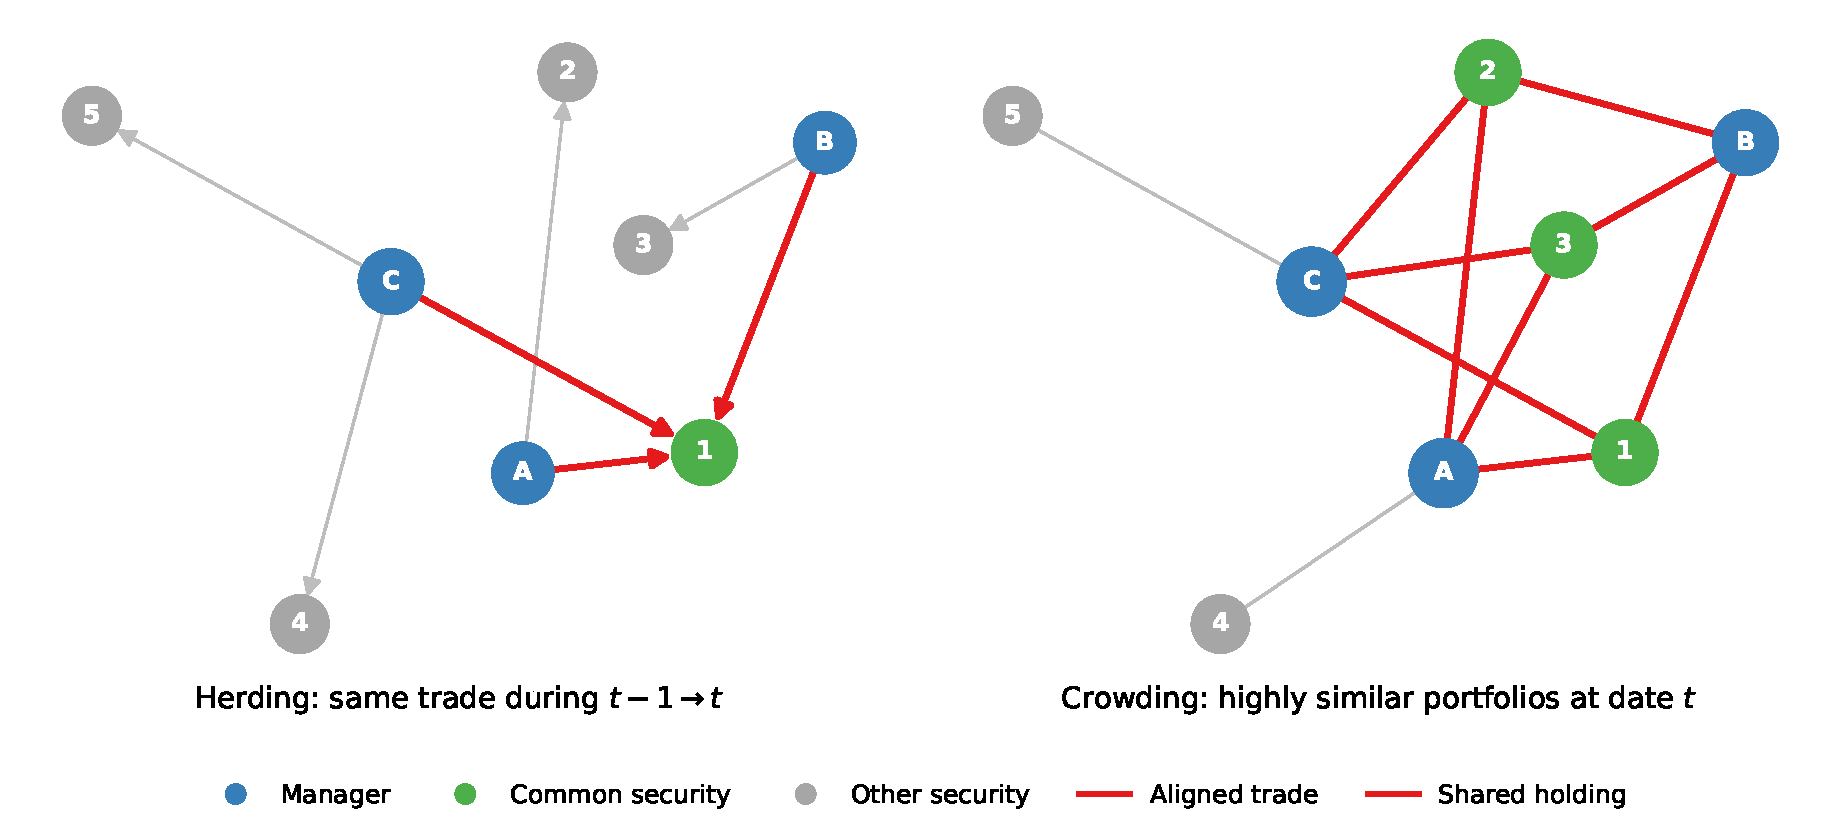
\includegraphics[width=0.9\textwidth]{08_04_herding_vs_crowding_networkx.pdf}
    \caption{Conceptual distinction between herding and crowding in institutional ownership networks.}
    \label{fig:herding-vs-crowding}
\end{figure}

\noindent
From a risk perspective, crowding becomes particularly relevant when the investors sharing a position are themselves similar. Aggregate institutional ownership alone does not reveal whether a stock is held by a diverse group of investors or by institutions with strongly overlapping portfolios. In the latter case, common shocks to investor capital, investment strategies, or risk constraints may generate correlated demand for liquidity. The ownership structure may consequently create an additional channel through which stress affecting investors can be transmitted to the securities they jointly hold. This intuition connects the literature on institutional ownership to the broader literature on flow-driven price pressure and fire sales, discussed in Section~\ref{sec:liquidity_fire_sales}.

More recent work has examined crowdedness directly as a security-level characteristic. \textcite{brown2022crowded} use hedge-fund position data to construct measures of security-level crowdedness and show that greater exposure to crowdedness is associated with downside tail risk and larger drawdowns during periods of market distress. Their results are important for the present analysis because they suggest that information contained in institutional portfolios may be relevant not only for expected returns but also for asymmetric downside outcomes. Related evidence from \textcite{lou2022comomentum} shows that excessive commonality in arbitrage activity can be associated with subsequent reversals, supporting the broader idea that crowded investment strategies may become destabilizing when many investors pursue similar positions.

\section{Liquidity, Price Pressure, and Fire Sales}
\label{sec:liquidity_fire_sales}

The previous section established that institutional positions and trading can be correlated across investors, and that such correlation is not, by itself, a source of risk. Correlated positioning becomes economically relevant only through a mechanism that translates common exposure into price movements unrelated to fundamentals. The literature on liquidity-driven trading and fire sales provides this mechanism.

\textcite{coval2007asset} show that mutual funds experiencing large outflows tend to reduce their existing positions for reasons unrelated to changes in the underlying fundamentals of the securities involved. When several distressed funds hold the same securities, their flow-driven sales can generate concentrated, non-fundamental selling pressure in those common holdings. Prices consequently decline not because information about future cash flows has changed, but because of a temporary imbalance between the demand for liquidity and the market's capacity to absorb the sales. They further document that these price effects are partially reversed over subsequent quarters, consistent with an interpretation in which the initial decline reflects price pressure rather than a permanent revision of fundamental value.

This mechanism has two implications that are central to the present thesis. First, it identifies overlapping institutional ownership, rather than aggregate institutional ownership alone, as a channel through which liquidity shocks are transmitted to securities: a stock is exposed to fire-sale risk to the extent that several of its owners may face correlated redemptions that force them to sell. Second, it implies that the relevant risk is asymmetric. Because the fire-sale mechanism considered here originates from forced selling in response to redemptions, its price impact predominantly affects the downside of the return distribution rather than being symmetric around zero. This asymmetry motivates the thesis's focus on downside risk, rather than on volatility more broadly, as the prediction target.
\section{Stock Price Fragility}
\label{sec:stock_price_fragility}

While the fire-sale literature explains how liquidity-driven trading can generate non-fundamental price pressure, it does not by itself identify which securities are most exposed to that pressure. \textcite{greenwood2011stock} address this question by introducing the concept of stock price fragility. They define an asset as fragile when it is susceptible to non-fundamental shifts in demand. Fragility can arise because ownership is concentrated or because the asset's owners face volatile or correlated liquidity shocks that cause them to trade simultaneously. It is therefore a property of the ownership base as a whole rather than of any individual investor. Empirically, the measure combines the composition of ownership with the estimated variance--covariance structure of owners' liquidity-driven trades. \textcite{greenwood2011stock} show that greater fragility strongly predicts higher subsequent total and idiosyncratic return volatility.

This formulation is related to crowding, but it contains more information than ownership concentration alone because it accounts for the volatility and correlation of owners' expected liquidity trades. More recent evidence moves toward the specific downside outcome examined in this thesis. Using hedge-fund position data, \textcite{brown2022crowded} construct security-level measures of crowdedness and show that stocks with greater exposure to crowdedness experience relatively larger drawdowns during periods of market distress. Their findings indicate that ownership-based vulnerability can become particularly visible in adverse market states and provide direct empirical motivation for using future maximum drawdown as the primary downside-risk target.
\section{Networks and Interconnectedness in Financial Markets}
\label{sec:ownership_networks}

The principal measures reviewed so far, from institutional ownership and crowding statistics to the fragility index of \textcite{greenwood2011stock}, share a common feature: each summarizes the ownership base of a stock through one or a small number of scalar quantities. A separate strand of the literature suggests that this compression may discard economically relevant information, since the manner in which market participants are connected can itself carry information about financial risk and its transmission.

\textcite{billio2012econometric} propose measures of financial connectedness based on principal-component analysis and Granger-causality networks constructed from the monthly returns of banks, broker-dealers, insurers, and hedge funds. They find that these sectors became highly interconnected over the preceding decade and that their connectedness measures can identify and quantify periods of financial crisis. Although this evidence concerns relationships among financial institutions rather than institutional ownership of individual stocks, it establishes a broader principle that motivates the present thesis: the topology of a financial network can contain information about systemic risk and the transmission of shocks.

Closer to the setting of this thesis, \textcite{anton2014connected} study stocks connected through common active mutual fund ownership. They show that greater shared ownership predicts higher return correlation after controlling for systematic risk exposures, style and sector similarity, and other stock-pair characteristics. Using the 2003 mutual fund trading scandal as a natural experiment, they also provide evidence that shared ownership causes this excess comovement rather than merely reflecting omitted similarities between connected firms. Their findings demonstrate that the identities of a stock's institutional owners, and particularly the connections created by common ownership, can have measurable asset-pricing consequences beyond those captured by conventional firm and stock-pair characteristics.

These findings motivate representing institutional holdings explicitly as a network rather than solely as a collection of independent stock-level indicators. In such a representation, institutional managers and securities form two distinct sets of nodes, with reported ownership positions defining the edges between them. This bipartite structure preserves the identity of each stock's owners and makes it possible to characterize how managers are connected through similar portfolios and how stocks are exposed to those connections. The resulting structure can be summarized through engineered features describing owner similarity, owner centrality, and concentration across manager communities, or it can be supplied directly to models that learn from the graph itself.
\section{Predictive Models and Graph-Based Learning}
\label{sec:graph_learning_finance}

Before considering graph-based models, it is important to distinguish the information supplied to a model from the flexibility with which that information is processed. Ridge regression provides a regularized linear benchmark that limits coefficient instability when predictors are correlated \parencite{hoerl1970ridge}. Gradient-boosted decision trees can instead learn nonlinear relationships and interactions without requiring them to be specified in advance, with XGBoost providing a scalable implementation of this approach \parencite{chen2016xgboost}. Comparing these model classes on identical feature sets therefore tests whether nonlinear flexibility improves prediction without attributing that improvement to the inclusion of additional ownership or network information.

Representing institutional ownership as a network, as motivated in Section~\ref{sec:ownership_networks}, introduces a separate modeling choice. Engineered network statistics can be added to conventional tabular models as additional predictors, whereas graph neural networks can learn representations directly from the graph. GraphSAGE constructs inductive node representations by aggregating information from neighboring nodes \parencite{hamilton2017inductive}. Graph attention networks (GATs) extend this approach by learning the relative importance assigned to different neighbors during aggregation \parencite{velickovic2018graph}. Applied to a manager--stock network, these methods allow a security's representation to depend on both its own characteristics and the managers connected to it, potentially capturing relational patterns that are not fully summarized by manually engineered network features.

Applications of graph learning to institutional holdings data are still limited and have emerged only recently. \textcite{izadifar2026institutional} represent Form 13F holdings as a discrete-time temporal bipartite graph connecting institutional managers and securities. They formulate the prediction of future portfolio weights as a node-affinity problem and show that their proposed model outperforms alternative dynamic graph-learning approaches. However, a simple exponential-moving-average benchmark achieves performance relatively close to that of the proposed model, highlighting the strong persistence of institutional portfolios and the importance of comparison with simple temporal benchmarks. Their study is particularly relevant to the present thesis because it demonstrates that Form 13F holdings can be represented and modeled directly as a dynamic graph.

A related application by \textcite{tagndynamic2026} constructs a multi-relational financial network combining price correlations, supply-chain relationships, and institutional co-holdings. The proposed temporal graph-attention framework integrates graph attention with recurrent learning to predict extreme stock-price volatility. Institutional co-holdings therefore enter the model as one of several potential channels of risk transmission, and the results indicate that the combined network improves extreme-volatility prediction relative to the study's non-graph benchmarks.

Together, these studies demonstrate the potential of graph learning in applications involving institutional ownership and financial risk, but they do not resolve the specific question examined in this thesis. \textcite{izadifar2026institutional} isolate the institutional ownership graph but predict future portfolio allocations rather than risk outcomes. Conversely, \textcite{tagndynamic2026} predict extreme volatility using several network layers simultaneously, preventing the contribution of institutional co-holdings from being identified separately. It therefore remains unclear whether institutional ownership topology, considered as a distinct source of information, improves the out-of-sample prediction of stock-level downside risk beyond market characteristics and conventional ownership measures, and whether learning directly from the graph provides an advantage over tabular models using engineered network features.

\section{Research Framework and Hypotheses}
\label{sec:research_framework}

The literature reviewed in this chapter supports a coherent framework linking institutional ownership to future downside risk. Institutional investors may hold overlapping or otherwise correlated positions, while common liquidity shocks can induce simultaneous trading and non-fundamental price pressure. A stock's vulnerability to this mechanism therefore depends not only on its aggregate institutional ownership, but also on the composition and structure of its investor base. Conventional ownership measures summarize selected aspects of that exposure, whereas a network representation preserves the relationships among managers and securities. Predictive models can then test whether this additional information improves out-of-sample forecasts and whether learning directly from the ownership graph provides an advantage over engineered network features.

This framework motivates five hypotheses organized around three dimensions: the information contained in ownership data, the ability of different models to exploit that information, and the economic relevance of the resulting predictions. The hypotheses are directional predictions to be evaluated empirically rather than maintained assumptions; failure to find an incremental benefit from ownership information or model complexity would therefore remain an informative result.

\begin{description}[leftmargin=2.2em, style=nextline]

      \item[H1 --- Conventional Ownership and Crowding.]
            Conventional institutional-ownership and crowding measures improve the out-of-sample prediction of stock-level downside risk relative to market characteristics alone.

      \item[H2 --- Ownership--Network Topology.]
            Engineered features describing ownership-network topology provide incremental predictive information beyond market characteristics and conventional ownership measures.

      \item[H3 --- Nonlinearity.]
            Nonlinear tabular models predict future downside risk more accurately than linear models estimated on the same feature sets.

      \item[H4 --- Graph Learning.]
            Graph-based models that learn directly from the manager--stock ownership network predict future downside risk more accurately than comparable tabular models, including those supplied with engineered network features.

      \item[H5 --- Economic Value.]
            The model-derived Fragility Score produces an economically meaningful out-of-sample ranking of subsequent downside risk and provides useful information for portfolio construction.

\end{description}

\noindent
Hypotheses H1 and H2 test the incremental information contained in conventional ownership measures and ownership-network topology. Hypotheses H3 and H4 examine whether greater model flexibility improves the extraction of information from a fixed feature set or directly from the ownership graph. Hypothesis H5 extends the evaluation beyond statistical accuracy to the economic significance of the resulting predictions. Chapter~\ref{chap:methodology} translates these hypotheses into explicit empirical comparisons, while Chapter~\ref{chap:results} reports the corresponding evidence.

\chapter{Methodology}
\label{chap:methodology}

SEC Form 13F holdings and CRSP market data are combined to construct a quarterly stock-level panel for predicting future downside risk. The chapter first describes the data sources, information-timing convention, and sample construction, before defining the prediction target and the market, ownership, and network features. It then presents feature engineering and selection, followed by the chronological samples, staged model-selection procedure, candidate models, and evaluation metrics. The remaining sections define the Fragility Score, portfolio evaluation, and robustness procedures.

\section{Data Sources and Sample Construction}
\label{sec:data_sources}

The empirical analysis combines three data sources. Institutional ownership is obtained from SEC Form 13F filings, through which institutional investment managers that exercise investment discretion over at least \$100 million in Section 13(f) securities report specified holdings quarterly \parencite{sec2023form13f}. Daily security prices, returns, trading volume, shares outstanding, and delisting information are obtained from CRSP \parencite{crsp2026stock}. Daily U.S. Fama--French five-factor and momentum returns are obtained from the Kenneth French Data Library and are used only for the factor-adjusted portfolio evaluation \parencite{fama2015five,carhart1997persistence,french2026library}.

The SEC and CRSP data form a stock-quarter panel covering reporting quarters from 2013~Q2 through 2026~Q1. Each observation is indexed by a security and the quarter-end date to which its reported ownership positions refer. Form 13F filings are generally due within 45 calendar days after quarter-end, so the holdings are not assumed to be public on the reporting date. The analysis instead uses a common information cutoff 45 calendar days after each quarter-end, rolled forward to the next U.S. business day when necessary.

Market predictors are constructed using only information observed strictly before the cutoff, while ownership and network predictors use only eligible Form 13F filings available by that date. Each forward outcome window begins on the first trading day afterward. A stock-quarter therefore represents ownership at quarter-end, but its prediction is formed only after the corresponding filings could have become public. Detailed filing-consolidation, security-mapping, and eligibility rules are reported in Appendix~\ref{app:sample_construction}.
\section{Target and Feature Construction}
\label{sec:feature_construction}

This section defines the forward downside-risk target and three groups of candidate predictors: market features, conventional ownership features, and engineered network features. The network features are derived from a quarterly manager--stock graph that preserves the identities and portfolio relationships underlying the reported holdings. All predictors use only information available by each stock-quarter's information cutoff, whereas the target is measured over the subsequent return window. Predictor-distribution diagnostics use the training sample, while full-panel target statistics are explicitly identified and reported only for descriptive purposes.

\subsection{Downside-Risk Target}
\label{sec:target_definition}

Motivated by the liquidity-driven price-pressure mechanism and the stock-price fragility literature reviewed in Sections~\ref{sec:liquidity_fire_sales} and~\ref{sec:stock_price_fragility}, the primary prediction target is a forward-looking measure of stock-level downside risk rather than a symmetric measure of return dispersion. Specifically, the target is the positive magnitude of a security's maximum drawdown over the 63 trading days following its information cutoff. Let $r_{i,q,t}$ denote the return of stock $i$ on day $t$ of quarter $q$'s forward window, and define cumulative wealth by
\begin{equation}
    \begin{aligned}
        W_{i,q,0}=1,
        \qquad
        W_{i,q,t}=\prod_{s=1}^{t}\left(1+r_{i,q,s}\right).
    \end{aligned}
    \label{eq:cumulative_wealth}
\end{equation}
\noindent
The target is
\begin{equation}
    \mathrm{MDD}_{i,q}
    = \max_{1\leq t\leq 63}
    \left(
    1-
    \frac{W_{i,q,t}}
    {\max_{0\leq u\leq t}W_{i,q,u}}
    \right),
    \label{eq:maximum_drawdown}
\end{equation}
\noindent
so larger values represent more severe losses. This horizon approximates one calendar quarter and aligns the prediction window with the quarterly frequency of Form 13F reporting. A target window is complete only if the market calendar contains all 63 subsequent trading days, and it is usable only if the security has at least 50 observed daily returns within that window or, when delisted before the window ends, an observed delisting return. For a delisted security, the observed delisting return is included as its final realized return and wealth is then held constant through the remainder of the window, which is equivalent to retaining the proceeds as cash. This rule excludes unresolved or data-sparse outcomes rather than imputing them.

As shown in Figure~\ref{fig:target-diagnostics}, the target distribution is right-skewed, with a mean of approximately 22\%, a median of about 17\%, and a 99th percentile close to 78\%, indicating a pronounced upper tail of severe drawdowns. The target also varies materially over time. The highest quarterly median occurs in 2019~Q4, whose forward window contains the February--March 2020 COVID-19 market sell-off \parencite{baker2020unprecedented} and reaches approximately 48\%. This episode illustrates that the target captures economically meaningful downside events.

\begin{figure}[!htbp]
    \centering
    \begin{subfigure}[t]{0.48\textwidth}
        \centering
        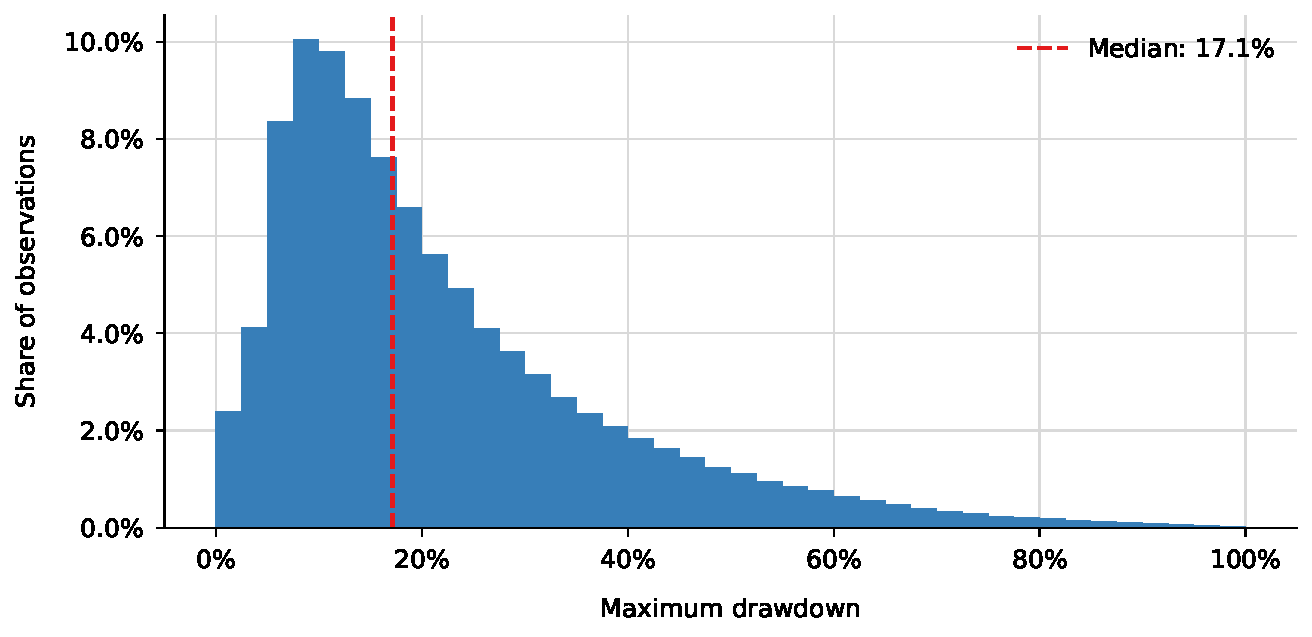
\includegraphics[width=\linewidth]{03_01_target_distribution_histogram.pdf}
        \caption{Cross-sectional target distribution.}
        \label{fig:target-distribution}
    \end{subfigure}
    \hfill
    \begin{subfigure}[t]{0.48\textwidth}
        \centering
        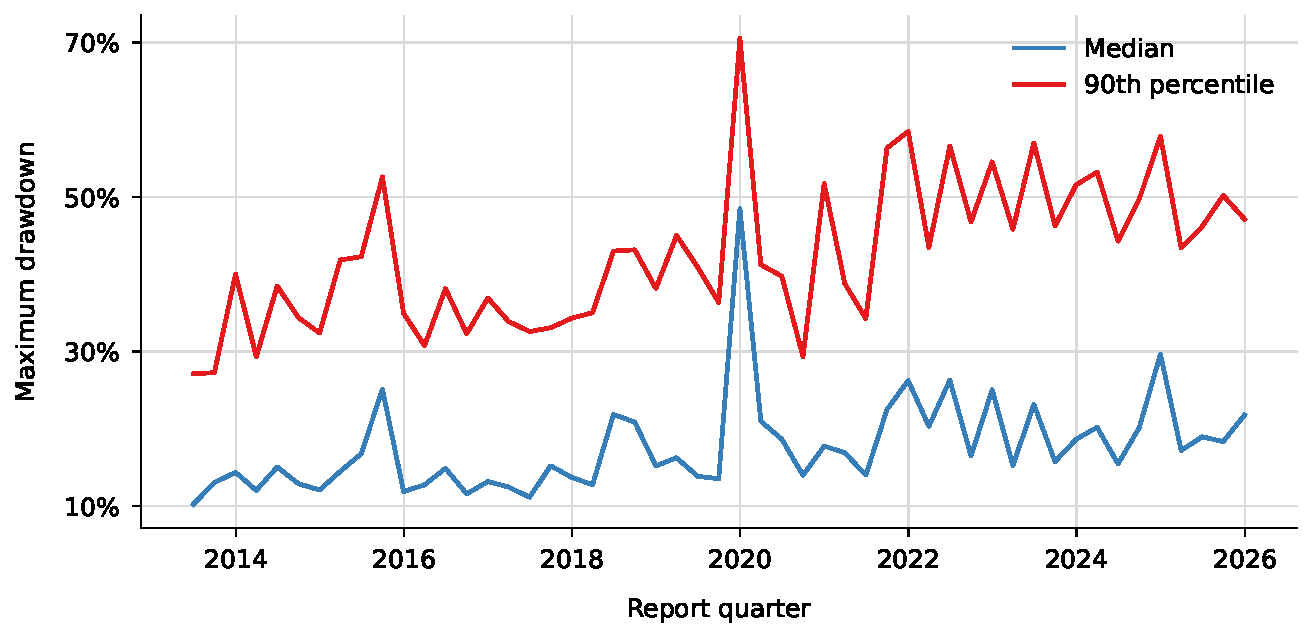
\includegraphics[width=\linewidth]{03_01_target_by_quarter.pdf}
        \caption{Target variation by reporting quarter.}
        \label{fig:target-by-quarter}
    \end{subfigure}
    \caption{Distribution and temporal variation of the forward 63-day maximum-drawdown target.}
    \label{fig:target-diagnostics}
\end{figure}

\noindent
Maximum drawdown is related to, but distinct from, other plausible downside measures. It is used as the primary target because it captures the cumulative peak-to-trough loss experienced within the prediction horizon. Alternative downside measures and prediction horizons are examined in Section~\ref{sec:robustness}. Comparable distributional statistics for the primary and alternative downside-risk targets are reported in Appendix~\ref{app:target_statistics}.

\subsection{Market Features}
\label{sec:market_features}

Nine candidate market features are constructed from CRSP daily data:

\begin{itemize}
    \item Size and liquidity: market capitalization and average daily dollar volume over 63 days;
    \item Returns and momentum: the 21-day return and momentum over the 252-to-21-day window;
    \item Risk: 63-day volatility, 63-day downside volatility, 252-day market beta, and 252-day maximum drawdown;
    \item Downside frequency: the share of negative returns over 63 days.
\end{itemize}

\noindent
These features provide the non-ownership benchmark against which the incremental value of conventional ownership measures and network information is evaluated. Size and liquidity capture differences in firms' capacity to absorb selling pressure; recent returns and momentum capture prevailing price dynamics; and the remaining variables describe total, downside, systematic, and path-dependent risk. All features are computed using information observed strictly before the corresponding information cutoff.

Exact variable definitions, minimum-data requirements, distributions, and temporal diagnostics are reported in Appendix~\ref{app:market_features}.

\subsection{Ownership Features}
\label{sec:crowding_measures}

Eleven conventional ownership features are constructed directly from the Form 13F holdings panel to test Hypothesis~H1, without using network-derived information:

\begin{itemize}
    \item Ownership scale: the institutional holder count and total reported institutional value;
    \item Ownership concentration: the Herfindahl--Hirschman index of reported holding shares and the share held by the five largest reported owners;
    \item Owner exposure: the mean and maximum portfolio weights assigned to the stock by its owners and the share of reporting managers that hold the stock;
    \item Changes in ownership: the quarter-over-quarter percentage changes in holder count and reported institutional value, together with the absolute changes in ownership concentration and the top-five ownership share.
\end{itemize}

\noindent
The scale measures describe the breadth and value of institutional participation, while the concentration measures capture how unevenly ownership is distributed across managers. The owner-exposure measures indicate how important the stock is within its owners' portfolios and how widely it is held across the reporting-manager universe. Finally, the change measures capture shifts in these ownership characteristics between consecutive quarters.

The four change measures are undefined when a security lacks a consecutive-quarter predecessor. Exact definitions, distributions, and temporal diagnostics are reported in Appendix~\ref{app:crowding_measures}.

\subsection{Bipartite Manager--Stock Graph}
\label{sec:bipartite_graph}

The conventional measures in Section~\ref{sec:crowding_measures} summarize each stock's ownership base through scalar statistics. To preserve the identities and portfolio relationships of the institutions behind those positions, the same Form 13F holdings are also represented as a quarterly network.

For each reporting quarter \(q\), institutional holdings form the bipartite graph

\begin{equation}
    G_q = \left(M_q \cup S_q, E_q\right),
    \qquad
    M_q \cap S_q = \varnothing,
    \label{eq:bipartite_graph}
\end{equation}

\noindent
where:

\begin{itemize}
    \item \(M_q\) is the set of reporting institutional managers;
    \item \(S_q\) is the set of held securities; and
    \item \(E_q \subseteq M_q \times S_q\) contains an edge \((m,i)\) whenever manager \(m\) reports holding security \(i\).
\end{itemize}

\noindent
Each edge carries two weights. The portfolio weight is the position's reported value divided by the manager's total reported portfolio value, while the ownership weight is the position's reported value divided by the security's total reported institutional value. The first measures the stock's importance to the manager; the second measures the manager's importance to the stock's reported ownership base.

Manager nodes contain portfolio value, security count, largest position weight, and portfolio concentration. Security nodes are matched to the stock-level market and conventional ownership measures described above, which are available as stock-node attributes. The scalar and network representations therefore describe the same retained holdings.

The ownership graph, manager-similarity graph, and manager communities are reconstructed independently for every reporting quarter. The resulting 52 point-in-time snapshots preserve changes in institutional portfolios without allowing later holdings to enter an earlier information set. Network growth and node-degree diagnostics are reported in Appendix~\ref{app:bipartite_graph}.

\subsection{Network Features}
\label{sec:network_features}

Managers are compared using the cosine similarity of their quarterly portfolio-weight vectors and connected to their nearest similar managers. Louvain community detection is then applied separately to each quarterly manager-similarity graph, so the resulting communities represent contemporaneous groups of managers with similar portfolios. These similarity and community assignments are aggregated across each stock's owners to construct the network features.

Eight stock-level features are derived from the ownership and manager-similarity networks:

\begin{itemize}
    \item Owner similarity: portfolio similarity among a stock's institutional owners;
    \item Owner centrality: value-weighted degree centrality of those owners;
    \item Neighbour similarity: value-weighted similarity between the owners and their nearest portfolio neighbours;
    \item Community breadth: number of manager communities represented among the owners;
    \item Community concentration: the ownership HHI across manager communities and the share held by the largest community; and
    \item Changes in topology: quarter-over-quarter changes in owner similarity and community concentration.
\end{itemize}

\noindent
Change features are undefined when a stock lacks a consecutive-quarter predecessor. The manager-similarity and community construction is documented in Appendix~\ref{app:manager_similarity}; exact network-feature definitions, distributions, and temporal diagnostics are reported in Appendix~\ref{app:network_features}.

\section{Feature Processing and Selection}
\label{sec:feature_engineering}

The candidate predictor set comprises nine market features, eleven conventional ownership features, and eight engineered network features. Feature processing proceeds in three stages. First, missingness is assessed across the fixed training, validation, and test samples. Second, strong feature redundancy is evaluated using the training sample only. Third, the retained variables are transformed and preprocessed as required by each model class. The resulting feature set is fixed before model selection, and no validation or test outcomes influence the choice of predictors.

\subsection{Feature Missingness}

Missingness is assessed across all 28 candidate predictors before transformation, imputation, or feature selection. All market features and all ownership and network level features are complete across the three modeling samples. Missing values are confined to the four ownership-change measures and the two network-change measures, which are undefined when a stock lacks an observation in the immediately preceding quarter.

Missingness in these variables is approximately 3\% in the training sample and below 0.2\% in both validation and test. The higher training share primarily reflects the beginning of the panel, where preceding-quarter histories are unavailable. Because this missingness is limited and arises mechanically from the construction of change variables, the affected observations are retained rather than deleted. Their treatment within the preprocessing pipeline is described in the following subsection. Complete feature-level missingness results are reported in Appendix~\ref{app:feature_processing}.

\subsection{Redundancy-Based Feature Selection}

Pairwise Spearman correlations are calculated separately within each training quarter and then averaged across quarters. Figure~\ref{fig:all-feature-correlations} shows strong relationships both within feature groups and across them. These correlations do not imply that the groups are economically identical, but they show that several candidate variables contain nearly the same cross-sectional information.

\begin{figure}[!htbp]
    \centering
    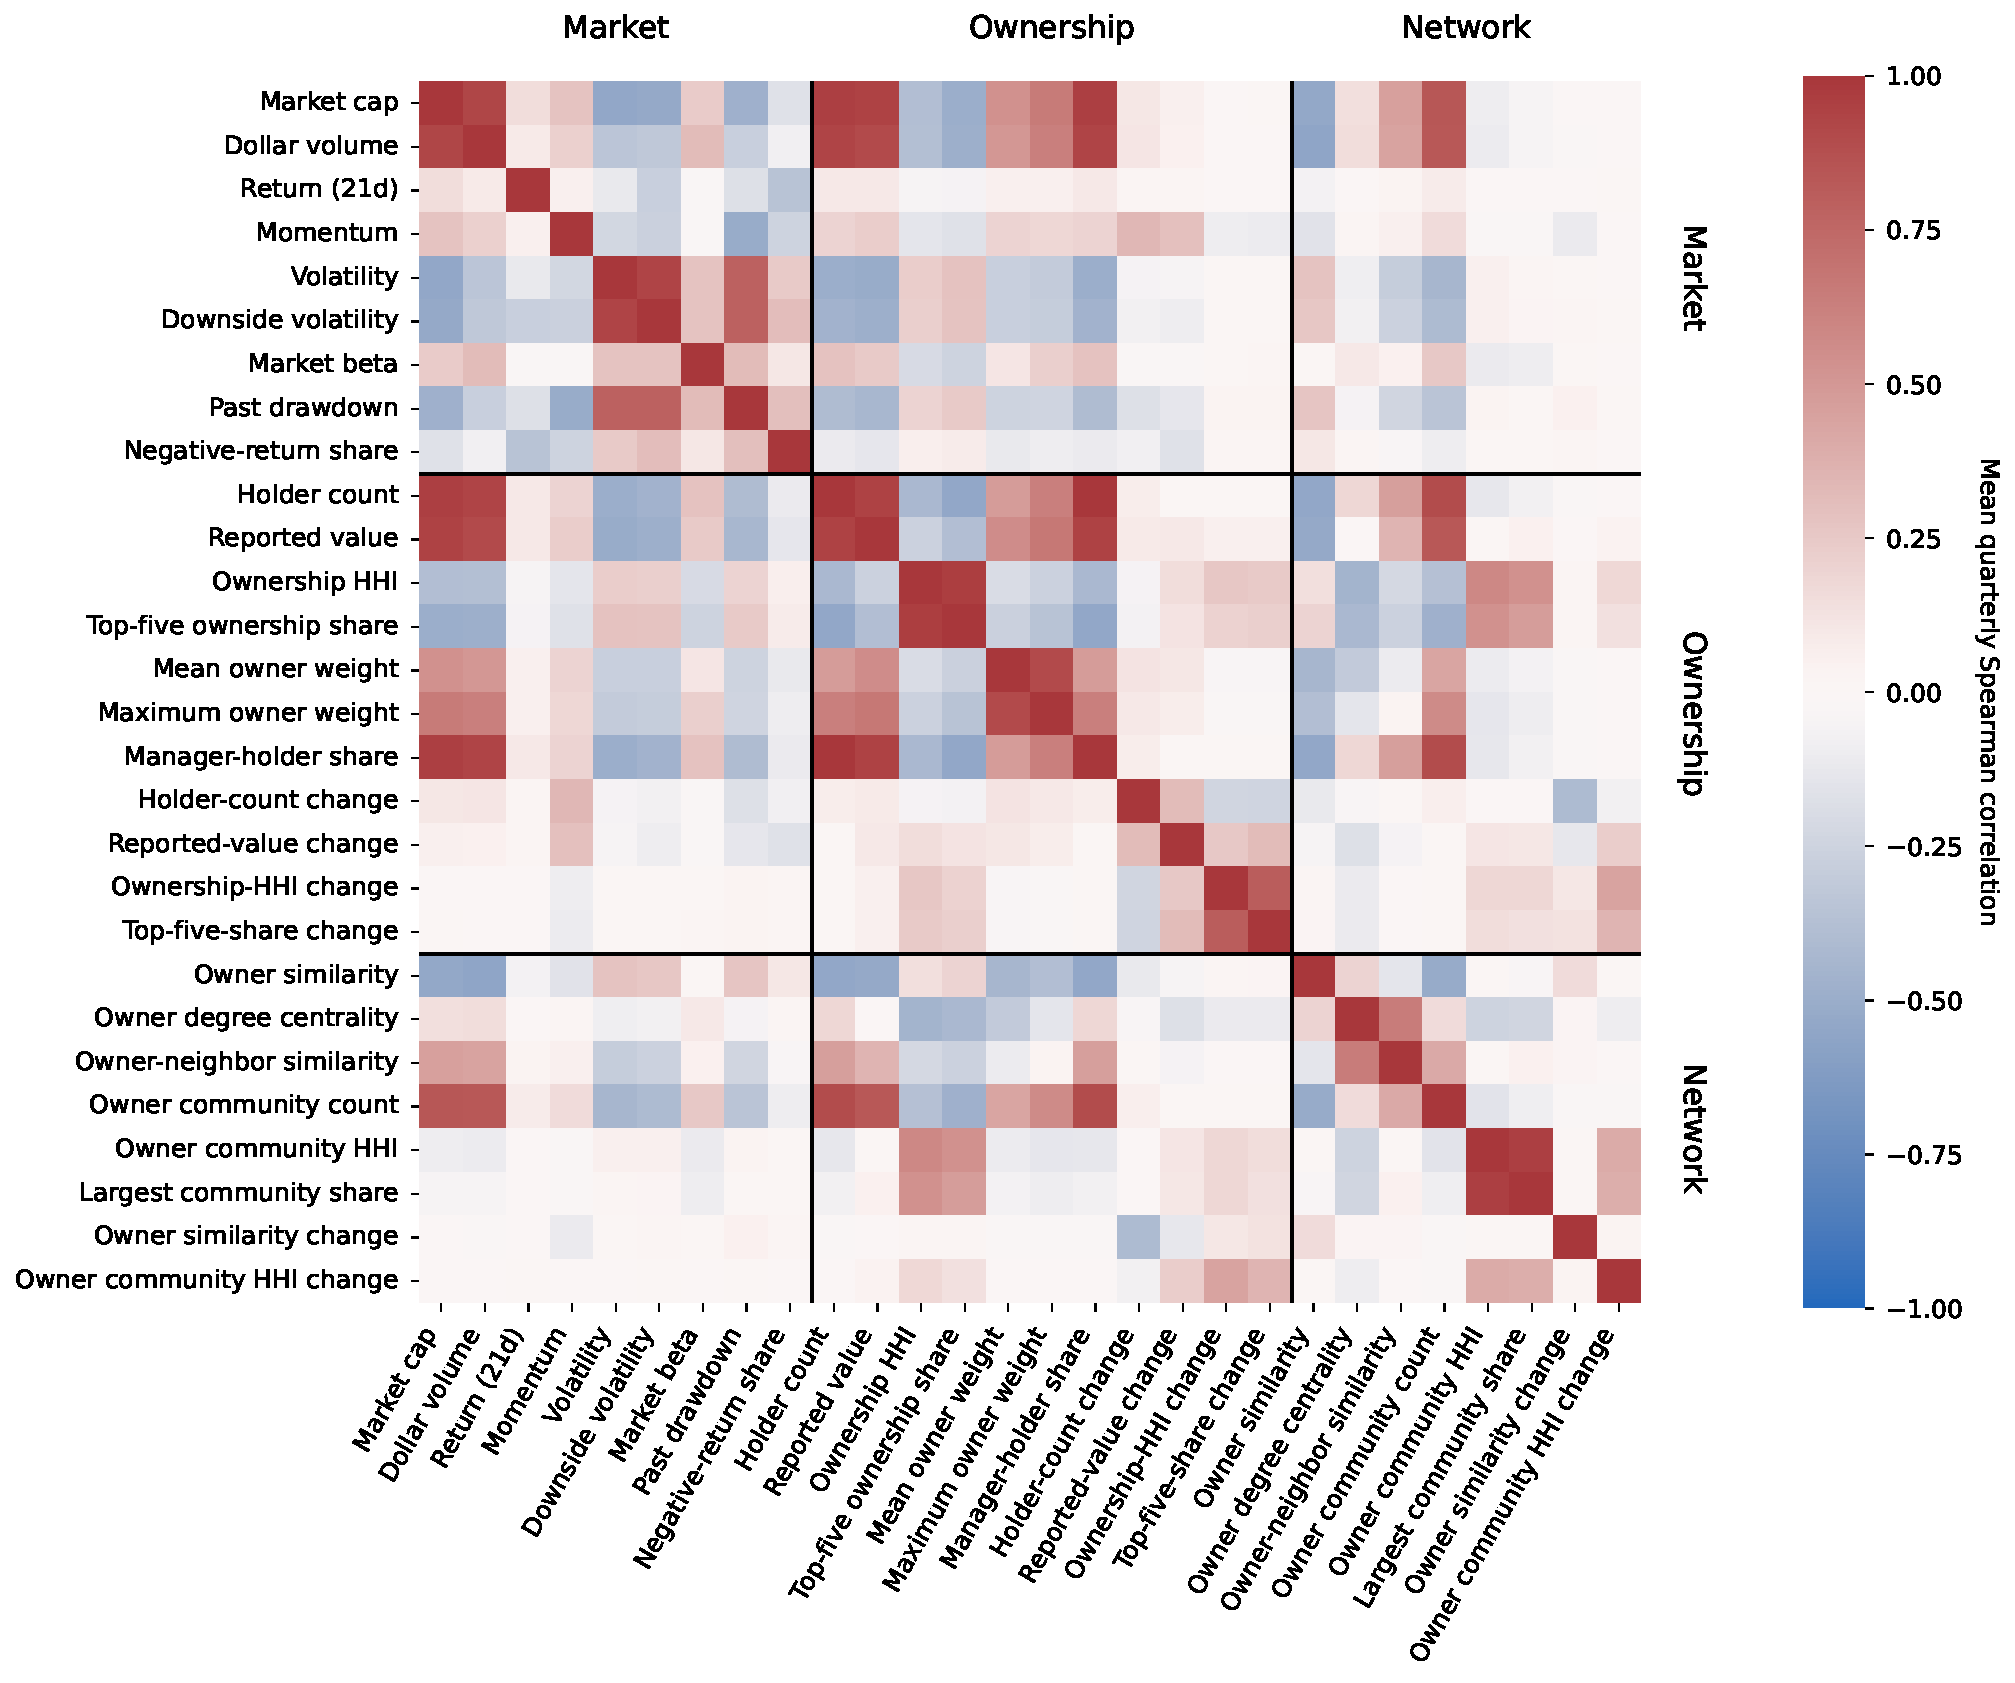
\includegraphics[width=0.95\textwidth]{04_03_all_feature_correlations.pdf}
    \caption[Correlations across candidate predictors]{Mean quarterly Spearman correlations among the candidate market, conventional ownership, and network features in the training sample.}
    \label{fig:all-feature-correlations}
\end{figure}

\noindent
Redundancy is reduced using a threshold of 0.80 for the absolute value of the mean quarterly correlation. Variables are first compared within each feature group, retaining the more interpretable representative of a highly correlated pair. Remaining cross-group correlations are then considered from the simplest to the most complex information set: market features first, conventional ownership features second, and engineered network features last. A more complex variable is removed when it largely reproduces information already represented by a simpler group. The target and all validation and test results are excluded from this decision. The complete set of feature pairs with absolute mean quarterly correlations above 0.70 is reported in Appendix~\ref{app:feature_correlations}, and the resulting selection decisions are summarized in Appendix~\ref{app:feature_selection_decisions}.

The resulting specification contains:

\begin{itemize}
    \item Seven market features: market capitalization, 21-day return, skip-month momentum, downside volatility, market beta, past maximum drawdown, and the share of negative returns;
    \item Five ownership features: ownership HHI, mean owner portfolio weight, and changes in holder count, reported value, and ownership HHI; and
    \item Six network features: owner similarity, owner degree centrality, owner neighbour similarity, owner-community HHI, and changes in owner similarity and community HHI.
\end{itemize}

\noindent
Ridge and XGBoost are estimated on nested subsets of these 18 predictors. The graph neural networks receive the same seven market and five ownership variables as stock-node attributes, but not the six engineered network features; they learn from the manager--stock graph and its ownership edges directly. The reduced feature set is fixed before model selection and is not revised in response to validation or test performance.

\subsection{Preprocessing}

After the final feature set is fixed, retained variables are prepared separately for each model. Market capitalization is transformed using \(\log(1+x)\) because its raw distribution is strongly right-skewed. For the graph-based models, manager portfolio value and manager security count receive the same transformation. No other retained tabular or node feature receives a logarithmic transformation.

The engineered network features used by the tabular network specifications are converted into within-quarter percentile ranks ranging from 0 to 1. Ranks are calculated across the full contemporaneous stock universe before applying modeling-eligibility restrictions, with tied observations receiving their average rank. Each value therefore represents a stock's relative position within that quarter's ownership network rather than the raw feature level. This reduces mechanical variation caused by changes in the size and composition of the network over time. The graph neural networks do not receive these engineered network features, since they learn directly from the manager--stock graph and its ownership edges.

Retained tabular predictors and graph-node features are clipped at the 1st and 99th percentiles estimated from the relevant fitting sample. Values outside these bounds are replaced by the corresponding percentile boundary, limiting the influence of extreme observations. Remaining missing values are replaced with fitting-sample medians. Ridge and the graph-based models additionally standardize their inputs using fitting-sample means and standard deviations, while XGBoost uses the clipped and imputed predictors without standardization.

For validation-stage estimation, all data-dependent preprocessing parameters are estimated from the training sample and applied unchanged to validation observations. Once the finalist specifications and their hyperparameters have been fixed using validation data, their preprocessing parameters are re-estimated from the combined training and validation samples and applied unchanged to the test observations. The test sample therefore does not influence any transformation, clipping bound, imputation value, or scaling parameter. Missingness and transformation diagnostics, together with the complete preprocessing rules, are reported in Appendix~\ref{app:feature_processing}.

\section{Predictive Modeling Design}
\label{sec:modeling_design}

The predictors retained in Section~\ref{sec:feature_engineering} define three nested tabular information sets: market features; market and conventional ownership features; and market, ownership, and engineered network features. Graph neural networks instead receive the retained market and ownership variables as stock-node attributes, but not the engineered network features, because they learn directly from the manager--stock graph and its ownership edges.

The predictive analysis proceeds through a sequence of validation-based comparisons. First, the three nested feature sets are evaluated separately within Ridge and XGBoost under common initial settings. Comparisons across feature sets test whether conventional ownership and engineered network features provide incremental predictive information (Hypotheses~H1 and~H2), while comparisons between Ridge and XGBoost on identical inputs test whether nonlinear flexibility improves prediction (Hypothesis~H3). One feature specification is retained within each model class. When validation differences are negligible, the simpler information set is preferred.

Second, the retained XGBoost specification is refined using the controlled tuning procedure described below, while Ridge retains its fixed penalty. Third, GraphSAGE, GAT, and Temporal GraphSAGE are compared under a common initial configuration, after which only the strongest graph architecture is tuned. Comparing the tuned graph specification with the tabular finalists tests whether learning directly from the ownership structure provides incremental predictive value (Hypothesis~H4).

The final validation comparison considers the retained linear, nonlinear, and graph-based specifications. Model selection is completed before the test sample is examined and considers the primary validation metric together with the consistency of the complementary metrics and model complexity. Additional complexity is retained only when it produces a material and consistent predictive improvement. Once the decision is fixed, the finalist specifications are refitted on the combined training and validation samples and evaluated once on the held-out test sample. Test performance is used to assess whether the validation evidence generalizes, not to reopen model selection.

\subsection{Chronological Samples and Model Selection}
\label{sec:chronological_samples}

After manager-quarter filings are consolidated, securities are mapped to historical CRSP records, and observations are checked for usable predictors and outcomes, eligible stock-quarters are assigned to fixed chronological training, validation, and test samples. Table~\ref{tab:modeling_samples} reports their sizes and coverage. Target distributions across the chronological modeling samples are reported in Appendix~\ref{app:chronological_samples}.

\begin{table}[H]
    \centering
    \caption{Chronological modeling samples}
    \label{tab:modeling_samples}
    \begin{tabular}{lrrl}
        \toprule
        Sample & Observations & Quarters & Coverage \\
        \midrule
        Training   & 123,791 & 34 & 2013 Q2--2021 Q3 \\
        Validation & 29,716 & 7 & 2022 Q1--2023 Q3 \\
        Test       & 30,511 & 8 & 2024 Q1--2025 Q4 \\
        \bottomrule
    \end{tabular}
\end{table}


\noindent
Chronological validation is used instead of random assignment because the empirical objective is to predict later quarters from earlier information. Random assignment would mix observations from different periods and would not reproduce this forward-looking setting. Because the primary target uses the 63 trading days after each information cutoff, 2021~Q4 and 2023~Q4 are purged at the training--validation and validation--test boundaries, respectively. This ensures that the outcomes used in one sample are resolved before the following sample begins.

The training sample is used to estimate candidate models. The validation sample is used to compare specifications, tune hyperparameters, and determine the number of boosting rounds or training epochs. During this process, the preprocessing parameters described in Section~\ref{sec:feature_engineering} are estimated from the training sample and applied unchanged to validation observations. Validation MAE is the primary selection metric. When competing specifications achieve materially similar MAE, the complementary metrics defined in Section~\ref{sec:evaluation_metrics}, together with model complexity, are used to prefer the more stable and parsimonious specification.

Once model selection has been completed using validation data, the finalist specifications are refitted on the combined training and validation samples. Their feature sets and hyperparameters, including the validation-selected number of boosting rounds or training epochs where applicable, remain fixed. Each finalist is then evaluated once on the held-out test sample to assess whether the validation evidence generalizes. Test performance does not reopen model selection.

\subsection{No-Information Benchmark}
\label{sec:no_information_benchmark}

The no-information benchmark predicts the fitting-sample mean target for every observation. For fitting sample \(\mathcal{F}\), its prediction \(\hat{y}_i\) is

\begin{equation}
    \hat{y}^{\,\mathrm{naive}}_i
    =
    \bar{y}_{\mathcal{F}}
    =
    \frac{1}{N_{\mathcal{F}}}
    \sum_{j\in\mathcal{F}} y_j,
    \label{eq:naive_mean}
\end{equation}

\noindent
where \(N_{\mathcal{F}}\) is the number of fitting observations. The benchmark uses no stock-level predictors and provides a direct reference for whether a fitted model improves on a constant forecast. For validation, \(\mathcal{F}\) is the training sample; for the final test comparison, it is the combined training and validation sample.

\subsection{Ridge Regression}
\label{sec:ridge_regression}

The linear model is Ridge regression \parencite{hoerl1970ridge}. Its coefficients solve

\begin{equation}
    \left(\hat{\beta}_0,\hat{\boldsymbol{\beta}}\right)
    =
    \arg\min_{\beta_0,\boldsymbol{\beta}}
    \left\{
    \sum_{i=1}^{N}
    \left(
    y_i-\beta_0-\mathbf{x}_i^{\prime}\boldsymbol{\beta}
    \right)^2
    +
    \alpha\lVert\boldsymbol{\beta}\rVert_2^2
    \right\},
    \label{eq:ridge_objective}
\end{equation}

\noindent
where \(\mathbf{x}_i\) contains the standardized predictors, \(\boldsymbol{\beta}\) contains their coefficients, and the intercept \(\beta_0\) is not penalized. The \(L_2\) penalty stabilizes coefficient estimates when predictors remain related after feature selection, while standardization makes the penalty comparable across variables measured on different scales. For simplicity, \(\alpha\) is fixed at 1 across all Ridge specifications. Holding the penalty constant ensures that differences across feature sets reflect changes in the information supplied to the model rather than simultaneous changes in regularization.

\subsection{XGBoost}
\label{sec:nonlinear_models}

The nonlinear tabular model is an XGBoost gradient-boosted tree ensemble \parencite{chen2016xgboost}. It builds predictions sequentially, with each additional tree seeking to reduce the errors left by the preceding trees. This structure allows nonlinear relationships and interactions among predictors to be learned without specifying them in advance.

A common prespecified configuration is used for the initial feature-set comparisons. The retained XGBoost specification is then refined through a controlled validation procedure that considers changes in learning rate and tree complexity, while the number of boosting rounds is determined through validation-based early stopping. XGBoost is trained using a squared-error objective, and validation MAE is the primary tuning metric. When configurations perform similarly, the faster-converging and less complex alternative is preferred. The complete initial settings and tuning configurations are reported in Appendix~\ref{app:model_specifications}.

\subsection{Graph-Based Models}
\label{sec:graph_models}

The graph-based analysis uses the quarterly manager--stock networks defined in Section~\ref{sec:bipartite_graph}. Stock nodes receive the retained market and conventional ownership features, while manager nodes receive portfolio value, security count, largest position weight, and portfolio concentration. Ownership edges carry portfolio weights and reported-ownership shares. The GNNs do not receive the engineered network features used by the tabular network-augmented specification, since they learn directly from the graph and its ownership edges.

Three architectures are considered. Weighted GraphSAGE \parencite{hamilton2017inductive} aggregates neighboring nodes using observed ownership-edge weights, while GAT \parencite{velickovic2018graph} learns attention weights from node and edge information. Both process each quarterly graph independently. Temporal GraphSAGE additionally uses a gated recurrent unit to carry stock-node states across consecutive quarters.

Figure~\ref{fig:weighted_graphsage_update} illustrates the principal elements of a manager-to-stock update in weighted GraphSAGE. The representation is conceptual; the model-specific message-passing and temporal-update equations are provided in Appendix~\ref{app:gnn_architectures}.


\begin{figure}[!htbp]
    \centering
    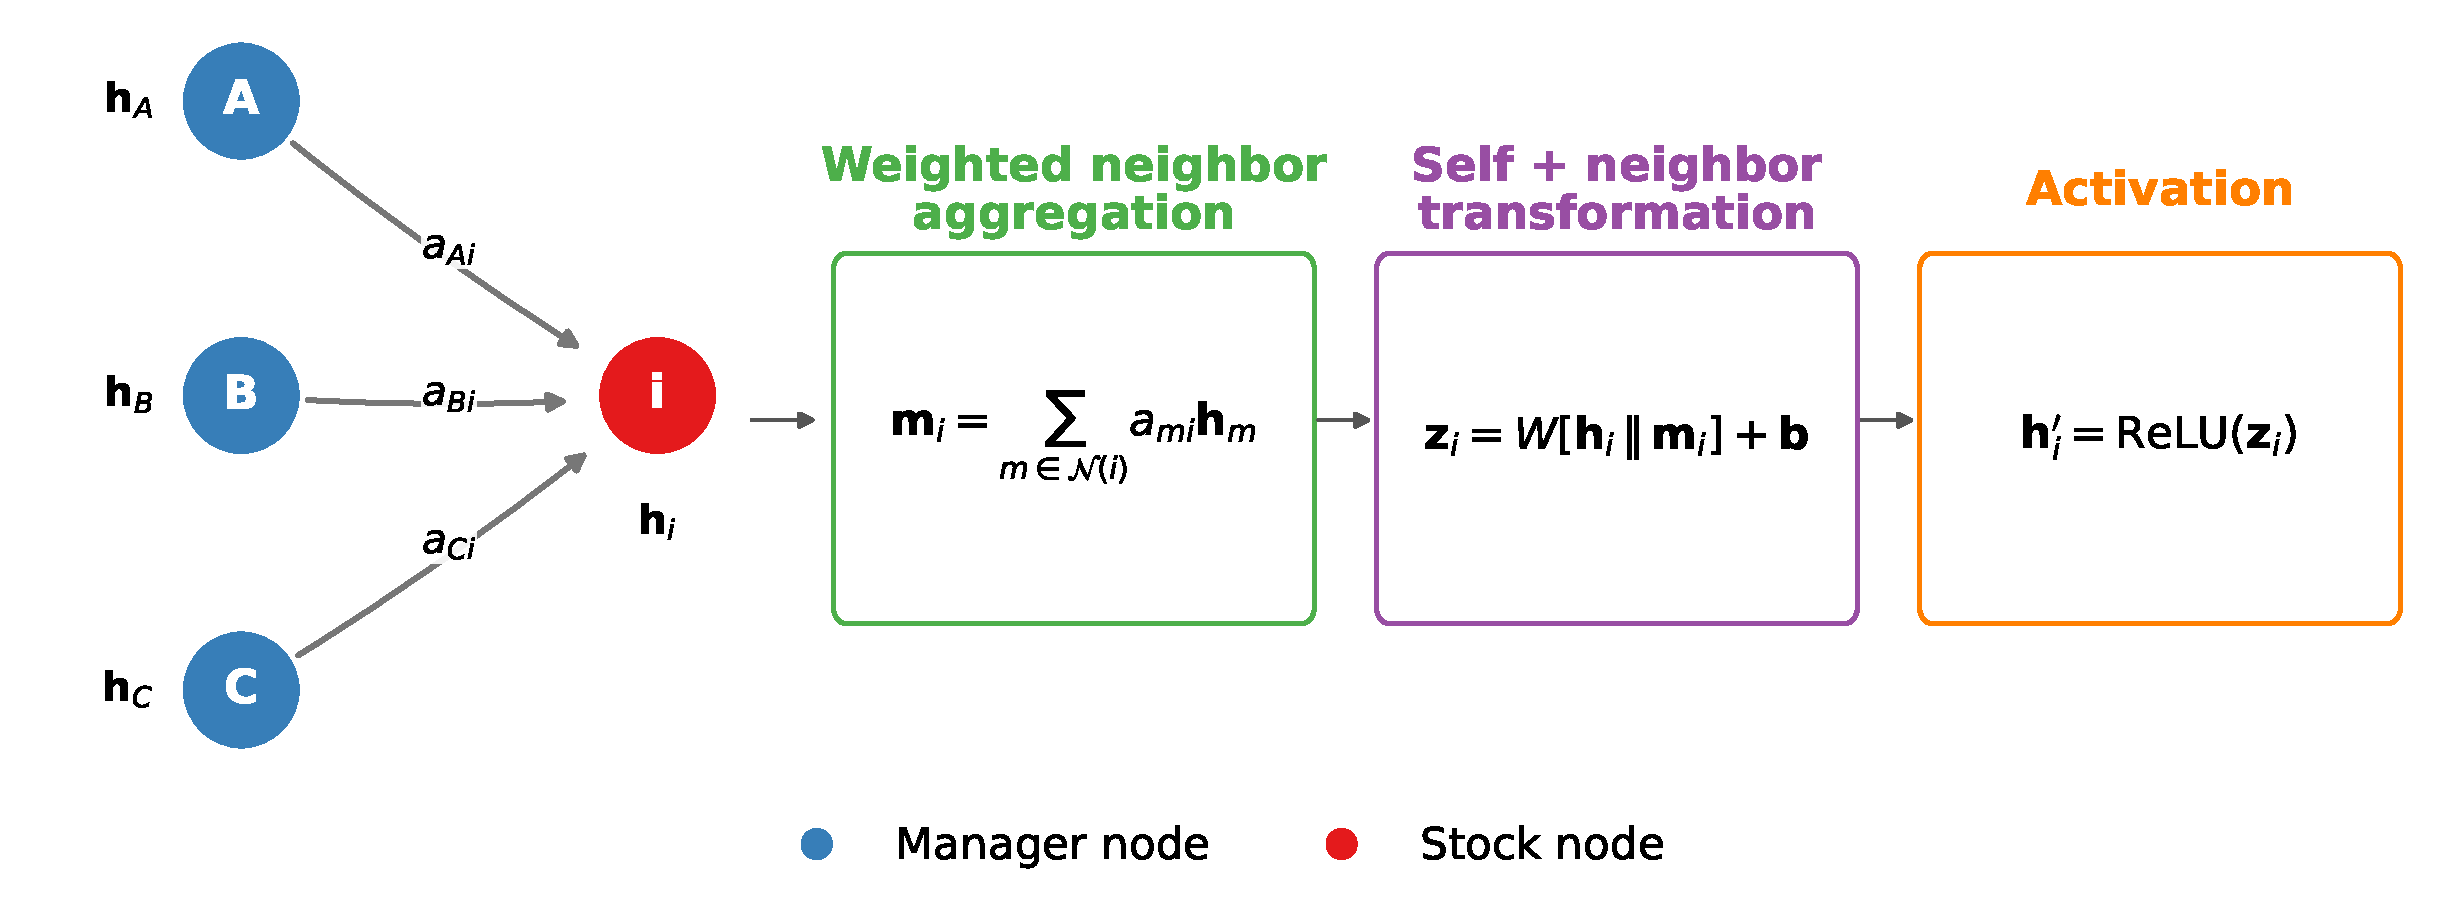
\includegraphics[width=\textwidth]{08_05_gnn_node_update.pdf}
    \caption[Weighted GraphSAGE message passing]{Weighted GraphSAGE update for a stock node using normalized ownership weights $a_{mi}\equiv o_{mi,q}$, with $\sum_{m\in\mathcal{N}(i)}a_{mi}=1$, followed by a learned transformation and nonlinear activation.}
    \label{fig:weighted_graphsage_update}
\end{figure}

\noindent
The three architectures are initially estimated under a common configuration and compared using validation MAE. Only the strongest architecture is subsequently refined through controlled changes in model capacity, regularization, and learning rate, while the number of training epochs is determined through validation-based early stopping. The resulting graph specification then enters the final validation comparison with the retained linear and nonlinear tabular specifications. Overall model selection follows the performance and parsimony criteria described in Section~\ref{sec:chronological_samples}.

The graph-modeling sequence contains 51 labeled snapshots because the final ownership snapshot has no resolved 63-day outcome. Purged snapshots may update temporal states but contribute no training loss. Complete model settings and tuning configurations are reported in Appendix~\ref{app:model_specifications}.

\subsection{Evaluation Metrics}
\label{sec:evaluation_metrics}

Every model predicts the continuous downside-risk target defined in Section~\ref{sec:target_definition}. Predictions are bounded between 0 and 1 before evaluation, corresponding to the feasible range of the maximum-drawdown target. Let \(y_i\) denote the realized target and \(\hat{y}_i\) its prediction for observation \(i\) in an evaluation sample of size \(N\). The primary quantitative selection metric is the mean absolute error,

\begin{equation}
    \mathrm{MAE}
    =
    \frac{1}{N}
    \sum_{i=1}^{N}
    \left|y_i-\hat{y}_i\right|.
    \label{eq:mae}
\end{equation}

\noindent
MAE expresses prediction error in the same units as the target and is less dominated by the target's severe upper tail than a squared-error criterion.

Two complementary magnitude-based metrics are also reported. Root mean squared error gives greater weight to large errors,

\begin{equation}
    \mathrm{RMSE}
    =
    \sqrt{
        \frac{1}{N}
        \sum_{i=1}^{N}
        \left(y_i-\hat{y}_i\right)^2
    },
    \label{eq:rmse}
\end{equation}

\noindent
while the coefficient of determination compares squared prediction error with a constant prediction equal to the evaluation-sample mean,

\begin{equation}
    R^2
    =
    1-
    \frac{
        \sum_{i=1}^{N}
        \left(y_i-\hat{y}_i\right)^2
    }{
        \sum_{i=1}^{N}
        \left(y_i-\bar{y}\right)^2
    },
    \label{eq:r_squared}
\end{equation}

\noindent
where \(\bar{y}\) is the mean realized target in that sample. An \(R^2\) below zero therefore indicates that the model performs worse under squared error than this constant benchmark.

For the Ridge feature-set comparison, the Akaike information criterion (AIC) and Bayesian information criterion (BIC) are additionally reported as in-sample complexity diagnostics. Because Ridge shrinks rather than eliminates coefficients, model complexity is measured using the effective degrees of freedom,

\begin{equation}
    d_{\alpha}
    =
    1+
    \sum_k
    \frac{s_k^2}{s_k^2+\alpha},
    \label{eq:ridge_effective_df}
\end{equation}

\noindent
where \(s_k\) are the singular values of the standardized design matrix and the additional unit represents the intercept. Let \(n\) denote the number of training observations and \(\mathrm{RSS}\) the training residual sum of squares. The information criteria are calculated as

\begin{equation}
    \begin{aligned}
        \mathrm{AIC}
         & =
        n\left[
            \log(2\pi)+1+
            \log\left(\frac{\mathrm{RSS}}{n}\right)
            \right]
        +2d_{\alpha}, \\
        \mathrm{BIC}
         & =
        n\left[
            \log(2\pi)+1+
            \log\left(\frac{\mathrm{RSS}}{n}\right)
            \right]
        +d_{\alpha}\log(n).
    \end{aligned}
    \label{eq:ridge_information_criteria}
\end{equation}

\noindent
These statistics are reported only for the linear feature-set comparison and do not determine model selection.

Because the economic analysis uses predictions to rank stocks within each quarter, ranking performance is evaluated separately. For every evaluation quarter \(q\), the Spearman correlation \(\rho_q\) is computed between predicted and realized downside risk across the \(N_q\) eligible stocks. The reported statistic is the equally weighted mean across the \(Q\) evaluated quarters,

\begin{equation}
    \overline{\rho}
    =
    \frac{1}{Q}
    \sum_{q=1}^{Q}
    \rho_q.
    \label{eq:mean_quarterly_spearman}
\end{equation}

\noindent
A value near zero indicates little systematic within-quarter ranking ability, whereas a positive value indicates that stocks assigned greater predicted fragility tend to experience larger subsequent drawdowns. This metric directly evaluates the within-quarter ranking that underlies the Fragility Score defined in Section~\ref{sec:fragility_score_construction}.

If XGBoost is selected, SHAP (SHapley Additive exPlanations) decomposes each fitted prediction into additive feature contributions relative to the model's expected output, summarizing their global importance and observation-level direction \parencite{lundberg2017unified}.

\section{Fragility Score Construction}
\label{sec:fragility_score_construction}

The predictive models produce a continuous estimate of forward 63-day maximum drawdown for each eligible stock-quarter. To obtain an interpretable cross-sectional risk ranking, these predictions are transformed into a stock-level \emph{Fragility Score}. For stock $i$ in quarter $q$, the score is

\begin{equation}
    \mathrm{FS}_{iq}
    = 100\frac{r_{iq}-1}{N_q-1},
    \label{eq:fragility_score}
\end{equation}

\noindent
where $r_{iq}$ is the ascending rank of the stock's predicted drawdown among the $N_q$ eligible stocks in that quarter. Tied predictions receive their average rank; if a quarter contains only one eligible stock, its score is set to 50.

The score lies between 0 and 100. When the extreme predictions are unique, the lowest receives 0 and the highest receives 100; tied predictions receive the score implied by their average rank. A score of 90 therefore means that the stock is predicted to be more fragile than approximately 90\% of the eligible universe in the same quarter. Ranking is performed separately within each quarter and uses only the contemporaneous cross-section of model predictions.

This transformation preserves relative ordering rather than the predicted level of drawdown. It is therefore suited to downside-risk sorting and portfolio applications, while the accuracy of the underlying magnitude predictions is evaluated separately using the error metrics. The primary economic evaluation applies the score to the model selected using the validation sample.

\section{Portfolio Evaluation Design}
\label{sec:portfolio_evaluation_design}

The Fragility Score is evaluated primarily as a downside-risk ranking rather than as a return-forecasting signal. Within each test quarter, eligible stocks are assigned to ten score groups, with Decile~1 containing the least fragile stocks and Decile~10 the most fragile. The primary comparison uses an equally weighted portfolio of all eligible stocks as an internal benchmark and a matched screened portfolio that excludes Decile~10. Because both portfolios are formed from the same initial universe using identical formation dates and weighting rules, their difference isolates the effect of excluding the stocks predicted to be most fragile.

\subsection{Quarterly Portfolio Risk Evaluation}

At the first trading day after each quarter's information cutoff, four portfolios are formed: all eligible stocks, the screened universe excluding Decile~10, Decile~1 alone, and Decile~10 alone. Constituents receive equal initial weights and are held for the following 63 trading days without re-ranking or rebalancing within the window. Individual stock weights are therefore allowed to evolve with realized returns. When a security delists after an observed delisting return, its subsequent return is set to zero, so the remaining proceeds are treated as cash rather than redistributed across surviving stocks.

The primary comparison is the difference in maximum drawdown between the screened and unscreened portfolios. Downside volatility and the positive magnitude of the worst five-day return provide supporting risk measures, while cumulative return is reported descriptively rather than treated as the principal success criterion. The isolated decile portfolios assess whether realized downside risk increases from the least-fragile to the most-fragile end of the ranking.

\subsection{Continuous Portfolio and Factor Evaluation}

The same signal is also evaluated over a continuous daily return series. Portfolios are reconstituted on the first trading day after each quarterly information cutoff and held without interim rebalancing until the next formation date. The final portfolio is held through the end of its 63-day target window. Performance is summarized using cumulative and annualized return, annualized volatility, the Sharpe ratio based on daily excess returns, maximum drawdown, and downside volatility. The CRSP total-market index is reported as an external reference, but it is not a matched benchmark because it has a different security universe and weighting scheme.

Factor-adjusted performance is estimated using both the capital asset pricing model \parencite{sharpe1964capital} and the Fama--French five-factor model augmented with momentum. For each fully invested portfolio \(p\), the general regression is

\begin{equation}
    R_{p,t}-R_{f,t}
    =
    \alpha_p
    +
    \boldsymbol{\beta}_p^{\prime}\mathbf{F}_t
    +
    \varepsilon_{p,t},
    \label{eq:factor_regression}
\end{equation}

\noindent
where \(\mathbf{F}_t\) contains the market excess return in the CAPM and the market, size, value, profitability, investment, and momentum factors in the augmented specification. The same regressions are estimated for the zero-investment screened-minus-unscreened portfolio using its return difference, without subtracting the risk-free rate. Alpha is annualized by multiplying the daily intercept by 252, and inference uses Newey--West standard errors with five trading-day lags \parencite{newey1987simple}.

As a supplementary test, a fully invested long position in Decile~1 is combined with a fully invested short position in Decile~10. The resulting zero-investment DFRAG-10 portfolio is rebalanced on the same quarterly schedule and evaluated with the same factor specifications, without subtracting the risk-free rate. It is interpreted as an exploratory measure of the return spread between the two extremes of predicted fragility, not as evidence of an immediately tradable factor. Its sensitivity to portfolio breadth, turnover, transaction costs, and factor exposures is examined in the next section.

\section{Robustness Design}
\label{sec:robustness}

The primary analysis combines the 63-day maximum-drawdown target, the validation-selected model specification, and the portfolio evaluation design described above. The robustness analysis varies one design choice at a time relative to this primary specification, allowing changes in the results to be attributed to a specific alternative rather than to several simultaneous modifications.

\subsection{Predictive Robustness}

Predictive robustness is assessed across alternative definitions and horizons of downside risk. The selected model class or architecture, feature set, and validation-chosen hyperparameters are held fixed, so no new model selection or tuning is performed. The model is re-estimated on the corresponding training and validation observations for each alternative outcome and then evaluated on the test sample. Two alternative 63-day outcomes are considered: downside volatility and the positive magnitude of the worst five-day return. Maximum drawdown is also reconstructed over shorter and longer horizons of 21 and 126 trading days.

All alternative outcomes use the same point-in-time information convention and usability principles as the primary target. The calendar definitions of the training, validation, and test periods remain fixed, but an observation is excluded from a given robustness sample if its alternative target window crosses the next sample boundary. This preserves the chronological separation for each horizon.

\subsection{Investment Robustness}

The portfolio evaluation is examined along six dimensions:

\begin{itemize}
    \item the screen excludes either the most fragile decile or the most fragile quintile;
    \item portfolio weighting changes from equal to market-value weights;
    \item transaction costs of 10, 25, and 50 basis points per unit of one-way turnover are deducted from gross returns;
    \item Newey--West inference for screened-minus-unscreened alpha is repeated with 5, 21, and 63 trading-day lags;
    \item the long--short portfolio is broadened from the extreme deciles (DFRAG-10) to the two least-fragile and two most-fragile deciles (DFRAG-20); and
    \item DFRAG-10 exposure is scaled using its lagged 63-day realized volatility toward a 15\% annualized target, with exposure capped at one so that the strategy is not leveraged.
\end{itemize}

\noindent
Each alternative is compared with the corresponding primary construction without changing the Fragility Score used to rank securities.


\chapter{Empirical Results}
\label{chap:results}

This chapter presents the empirical evidence in the order in which the modeling decisions are made. It first compares the predictive contribution of the three feature groups within the linear and nonlinear models, then reports the tuning of the retained nonlinear and graph-based specifications. The final linear, nonlinear, and graph-based candidates are compared on the validation sample, where the overall model selection is fixed. All three finalists are subsequently refitted on the combined training and validation samples and evaluated once on the held-out test period without reopening the selection decision. The chapter then examines the selected model's interpretation, prediction errors, robustness, the Fragility Score, and its portfolio applications. It concludes by relating the evidence to the five research hypotheses.

\section{Feature-Set Comparison}
\label{sec:feature_set_results}

The first comparison examines whether conventional ownership and engineered network features improve prediction beyond the retained market variables. The three nested feature sets are evaluated separately within Ridge and XGBoost. Each specification is estimated on the training sample and assessed on the validation sample using a common configuration within its model class. This isolates the information supplied by the features from differences in model flexibility and hyperparameter settings.

\subsection{Ridge Feature-Set Comparison}
\label{sec:linear_feature_results}

Table~\ref{tab:ridge-feature-set-validation} reports the Ridge results, using MKT for market features, OWN for conventional ownership features, and NTW for engineered network features. Adding conventional ownership variables lowers validation MAE only slightly, and the engineered network variables provide a still smaller additional change. AIC and BIC favor the richer specifications because their small in-sample improvements are measured over a large training sample. They are reported as complementary complexity-adjusted diagnostics, while the retained specification is chosen from validation performance and parsimony. On that basis, the additional variables do not produce a material out-of-sample gain.

\begin{table}[!htbp]
\centering
\footnotesize
\setlength{\tabcolsep}{4pt}
\caption{Ridge validation performance and training-sample complexity diagnostics across feature sets.}
\label{tab:ridge-feature-set-validation}
\begin{tabular}{lrrrrrrr}
\toprule
Specification & $\mathrm{MAE}_{\mathrm{train}}$ & $\mathrm{MAE}_{\mathrm{val}}$ & $\mathrm{RMSE}$ & $R^2$ & $\overline{\rho}$ & AIC & BIC \\
\midrule
\textbf{MKT} & \textbf{0.0869} & \textbf{0.0959} & \textbf{0.1337} & \textbf{0.449} & \textbf{0.747} & \textbf{-169,214} & \textbf{-169,136} \\
MKT + OWN & 0.0869 & 0.0956 & 0.1334 & 0.452 & 0.746 & -169,471 & -169,344 \\
MKT + OWN + NTW & 0.0868 & 0.0956 & 0.1332 & 0.453 & 0.746 & -169,637 & -169,452 \\
\bottomrule
\end{tabular}
\end{table}


\noindent
Given these small differences, the market-only feature set is retained for the linear finalist. This is a parsimony decision: the ownership and network variables produce minor numerical improvements in MAE, but not a meaningful change in ranking performance. Validation errors across realized-drawdown deciles for the three Ridge specifications are reported in Appendix~\ref{app:linear_feature_set_diagnostics}.

\subsection{XGBoost Feature-Set Comparison}
\label{sec:nonlinear_feature_results}

Table~\ref{tab:xgboost-feature-set-validation} repeats the comparison using XGBoost under the same initial configuration. Conventional ownership features again produce a small reduction in validation MAE, while adding engineered network features does not improve on the ownership-augmented specification. The three specifications remain very close in both $R^2$ and rank correlation.

\begin{table}[!htbp]
\centering
\footnotesize
\setlength{\tabcolsep}{4pt}
\caption{XGBoost validation performance across feature sets.}
\label{tab:xgboost-feature-set-validation}
\begin{tabular}{lrrrrrr}
\toprule
Specification & Best round & $\mathrm{MAE}_{\mathrm{train}}$ & $\mathrm{MAE}_{\mathrm{val}}$ & $\mathrm{RMSE}$ & $R^2$ & $\overline{\rho}$ \\
\midrule
\textbf{MKT} & \textbf{176} & \textbf{0.0836} & \textbf{0.0950} & \textbf{0.1317} & \textbf{0.466} & \textbf{0.749} \\
MKT + OWN & 175 & 0.0833 & 0.0943 & 0.1305 & 0.475 & 0.751 \\
MKT + OWN + NTW & 140 & 0.0835 & 0.0946 & 0.1306 & 0.474 & 0.750 \\
\bottomrule
\end{tabular}
\end{table}


\noindent
The ownership variables therefore contain some incremental validation signal, but the improvement is too small to justify retaining the larger feature set for the subsequent model-class comparison. The market-only specification is retained and tuned in the next section. This evidence provides limited support for Hypothesis~H1 and no consistent support for Hypothesis~H2. Validation errors across realized-drawdown deciles for the three XGBoost specifications are reported in Appendix~\ref{app:nonlinear_feature_set_diagnostics}.

\section{XGBoost Tuning}
\label{sec:xgboost_tuning_results}

The retained market-only XGBoost model is refined through the controlled tuning procedure described in Section~\ref{sec:nonlinear_models}. Three configurations are compared: the initial model with a learning rate of 0.05 and depth three, a faster-learning specification with a rate of 0.10 and the same depth, and a deeper specification with a rate of 0.10 and depth four. Table~\ref{tab:xgboost-tuning-comparison} reports their training and validation performance. The selected configuration is shown in bold.

\begin{table}[!htbp]
\centering
\footnotesize
\setlength{\tabcolsep}{3.5pt}
\caption{Validation performance of the controlled XGBoost configurations.}
\label{tab:xgboost-tuning-comparison}
\begin{tabular}{rrrrrrrr}
\toprule
$\eta$ & Depth & Best round & $\mathrm{MAE}_{\mathrm{train}}$ & $\mathrm{MAE}_{\mathrm{val}}$ & $\mathrm{RMSE}$ & $R^2$ & $\overline{\rho}$ \\
\midrule
0.05 & 3 & 176 & 0.0836 & 0.0950 & 0.1317 & 0.466 & 0.749 \\
\textbf{0.10} & \textbf{3} & \textbf{90} & \textbf{0.0836} & \textbf{0.0951} & \textbf{0.1317} & \textbf{0.466} & \textbf{0.748} \\
0.10 & 4 & 54 & 0.0835 & 0.0952 & 0.1316 & 0.466 & 0.748 \\
\bottomrule
\end{tabular}
\end{table}


\noindent
The three configurations achieve nearly identical validation performance. Figure~\ref{fig:xgboost-base-selected-learning-curve} compares the initial and selected learning curves. Increasing the learning rate from 0.05 to 0.10 reduces the validation-selected number of boosting rounds from 176 to 90 without materially changing validation error, while increasing tree depth provides no further gain. The depth-three model with a learning rate of 0.10 is therefore retained for its faster convergence and lower complexity. Its complete parameter specification is reported in Appendix~\ref{app:xgboost_tuning_details}.

\begin{figure}[!htbp]
    \centering
    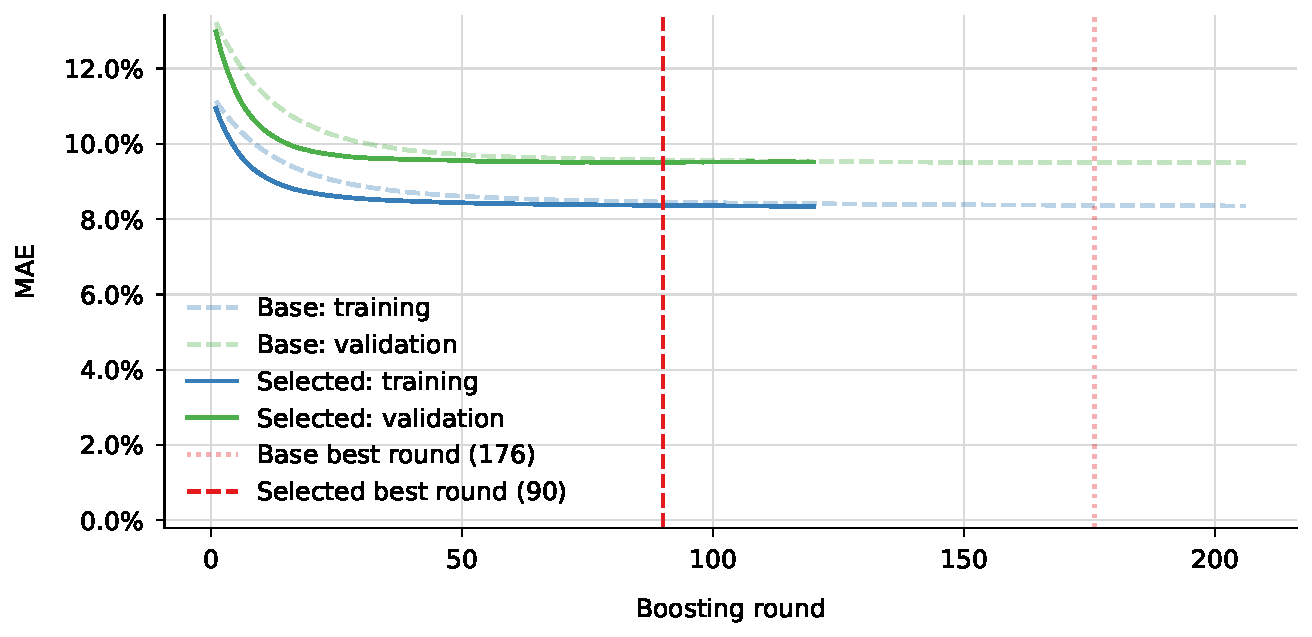
\includegraphics[width=0.82\textwidth]{04_02_xgboost_base_vs_selected_learning_curve.pdf}
    \caption[Learning curves for the initial and selected XGBoost configurations]{Training and validation MAE for the initial and selected market-only XGBoost configurations. The initial curves are semi-transparent, and the vertical lines mark each configuration's validation-selected boosting round.}
    \label{fig:xgboost-base-selected-learning-curve}
\end{figure}

\section{GNN Architecture Comparison}
\label{sec:gnn_results}

GraphSAGE, GAT, and Temporal GraphSAGE are first trained under a common initial configuration. Table~\ref{tab:gnn-architecture-comparison} shows that Temporal GraphSAGE achieves the lowest validation MAE and RMSE and the highest validation $R^2$. Its advantage over the two static architectures is consistent with useful information in stock states carried across quarterly ownership snapshots. Temporal GraphSAGE is therefore retained for tuning.

\begin{table}[!htbp]
\centering
\footnotesize
\setlength{\tabcolsep}{4pt}
\caption{Validation performance of the three GNN architectures.}
\label{tab:gnn-architecture-comparison}
\begin{tabular}{lrrrrrr}
\toprule
Architecture & Best epoch & $\mathrm{MAE}_{\mathrm{train}}$ & $\mathrm{MAE}_{\mathrm{val}}$ & $\mathrm{RMSE}$ & $R^2$ & $\overline{\rho}$ \\
\midrule
GraphSAGE & 28 & 0.0829 & 0.0985 & 0.1416 & 0.383 & 0.738 \\
GAT & 26 & 0.0844 & 0.0992 & 0.1418 & 0.381 & 0.739 \\
\textbf{Temporal GraphSAGE} & \textbf{23} & \textbf{0.0821} & \textbf{0.0945} & \textbf{0.1345} & \textbf{0.442} & \textbf{0.746} \\
\bottomrule
\end{tabular}
\end{table}


\noindent
The common architecture parameters and the individual learning curves are reported in Appendix~\ref{app:gnn_architecture_details}.

\subsection{Temporal GraphSAGE Tuning}
\label{sec:temporal_graphsage_tuning}

The selected base architecture is compared with four controlled variants that change its hidden dimension, learning rate, or dropout. Table~\ref{tab:temporal-graphsage-tuning-comparison} reports the five configurations. Expanding the hidden dimension from 16 to 32 produces a small reduction in validation MAE, whereas a higher learning rate, greater dropout, or a further increase in hidden dimension does not improve performance. The configuration with 32 hidden dimensions, a learning rate of 0.001, and dropout of 0.20 is therefore retained.

\begin{table}[!htbp]
\centering
\footnotesize
\setlength{\tabcolsep}{2.5pt}
\caption{Validation performance of the Temporal GraphSAGE configurations.}
\label{tab:temporal-graphsage-tuning-comparison}
\begin{tabular}{rrrrrrrrr}
\toprule
Hidden & $\eta$ & Dropout & Best epoch & $\mathrm{MAE}_{\mathrm{train}}$ & $\mathrm{MAE}_{\mathrm{val}}$ & $\mathrm{RMSE}$ & $R^2$ & $\overline{\rho}$ \\
\midrule
16 & 0.001 & 0.20 & 23 & 0.0821 & 0.0945 & 0.1345 & 0.442 & 0.746 \\
16 & 0.010 & 0.20 & 26 & 0.0837 & 0.0976 & 0.1372 & 0.420 & 0.735 \\
\textbf{32} & \textbf{0.001} & \textbf{0.20} & \textbf{28} & \textbf{0.0813} & \textbf{0.0941} & \textbf{0.1348} & \textbf{0.440} & \textbf{0.748} \\
32 & 0.001 & 0.30 & 20 & 0.0821 & 0.0943 & 0.1347 & 0.441 & 0.746 \\
64 & 0.001 & 0.30 & 4 & 0.0888 & 0.0962 & 0.1360 & 0.430 & 0.733 \\
\bottomrule
\end{tabular}
\end{table}


\noindent
Figure~\ref{fig:temporal-graphsage-base-selected-learning-curve} compares the base and selected learning curves. The selected model reaches its minimum validation error at epoch 28, after which training error continues to decline without a corresponding validation improvement. Together with the tuning results, this pattern indicates limited gains from additional capacity within the configurations tested.

\begin{figure}[!htbp]
    \centering
    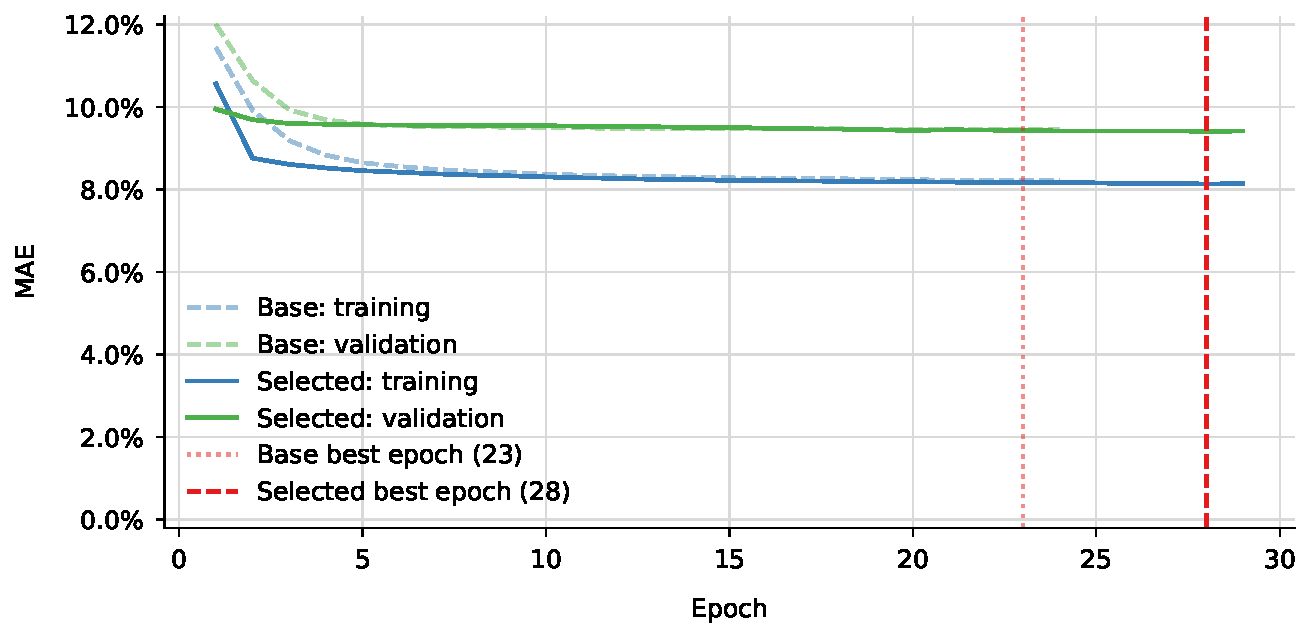
\includegraphics[width=0.82\textwidth]{04_04_temporal_graphsage_base_vs_selected_learning_curve.pdf}
    \caption[Learning curves for the base and selected Temporal GraphSAGE models]{Training and validation MAE for the base and selected Temporal GraphSAGE configurations. The base curves are semi-transparent, and the vertical lines mark each configuration's validation-selected epoch.}
    \label{fig:temporal-graphsage-base-selected-learning-curve}
\end{figure}

\noindent
The selected model's complete parameter specification and the individual tuning curves are reported in Appendix~\ref{app:gnn_tuning_details}. Whether the temporal architecture's validation advantage justifies its additional complexity is assessed against the tabular finalists in the next section.

\section{Final Validation Comparison and Model Selection}
\label{sec:final_validation_comparison}

The final validation comparison contains one representative of each model class: Ridge and tuned XGBoost using market features, and tuned Temporal GraphSAGE. Table~\ref{tab:finalist-validation-performance} reports their performance before any test result is examined.

\begin{table}[!htbp]
\centering
\footnotesize
\caption{Validation performance of the three finalist models.}
\label{tab:finalist-validation-performance}
\begin{tabular}{lrrrrr}
\toprule
Model & $\mathrm{MAE}_{\mathrm{train}}$ & $\mathrm{MAE}_{\mathrm{val}}$ & $\mathrm{RMSE}$ & $R^2$ & $\overline{\rho}$ \\
\midrule
Temporal GraphSAGE & 0.0813 & 0.0941 & 0.1348 & 0.440 & 0.748 \\
\textbf{XGBoost} & \textbf{0.0836} & \textbf{0.0951} & \textbf{0.1317} & \textbf{0.466} & \textbf{0.748} \\
Ridge & 0.0869 & 0.0959 & 0.1337 & 0.449 & 0.747 \\
\bottomrule
\end{tabular}
\end{table}


\noindent
Temporal GraphSAGE records the lowest validation MAE, but the difference from XGBoost is less than one tenth of a percentage point. XGBoost has the lower RMSE and higher $R^2$, while the two models have essentially identical rank correlations. Ridge remains competitive but is weaker than XGBoost on each reported validation metric, providing modest support for Hypothesis~H3.

Figure~\ref{fig:finalist-validation-deciles} confirms that the three models make errors in the same parts of the outcome distribution. Temporal GraphSAGE has a small average-MAE advantage, but none of the models resolves the sharp increase in error among the most severe realized drawdowns.

\begin{figure}[!htbp]
    \centering
    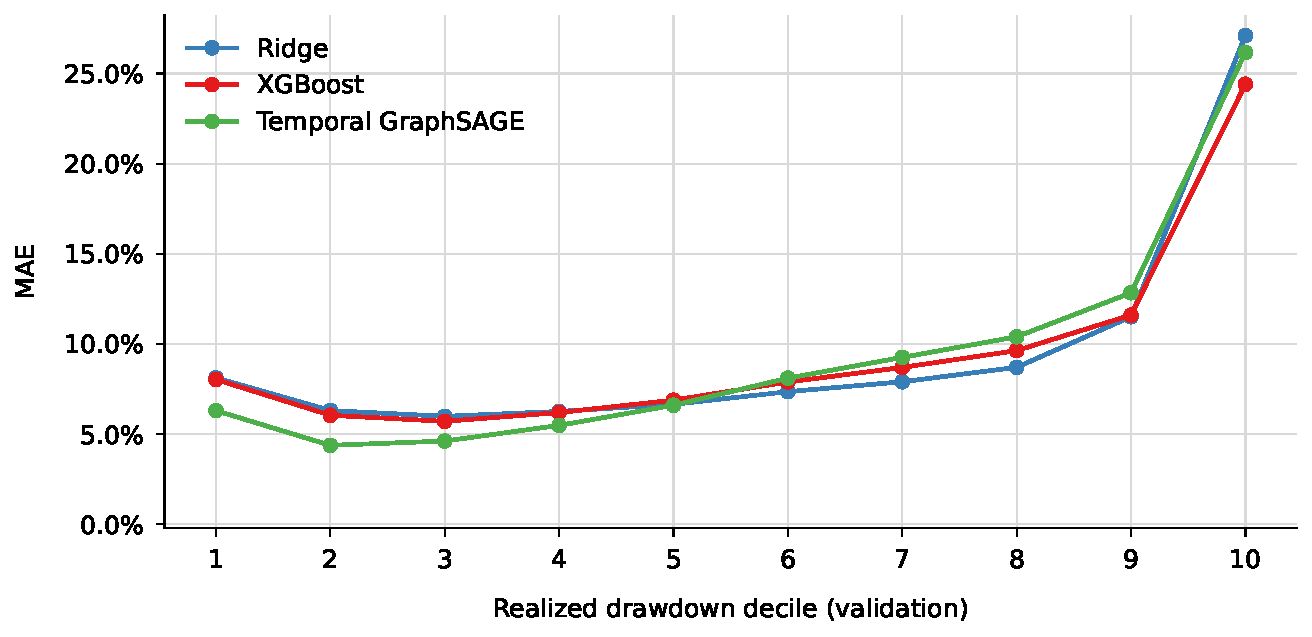
\includegraphics[width=0.82\textwidth]{04_07_validation_mae_by_realized_drawdown_decile.pdf}
    \caption[Validation errors across the finalist models]{Validation MAE across realized-drawdown deciles for market-only Ridge, market-only XGBoost, and Temporal GraphSAGE.}
    \label{fig:finalist-validation-deciles}
\end{figure}

\noindent
Market-only XGBoost is therefore selected before the test sample is examined. Although Temporal GraphSAGE achieves a marginally lower validation MAE, XGBoost offers comparable ranking performance, stronger RMSE and $R^2$, and substantially lower implementation complexity. The validation evidence therefore provides mixed rather than conclusive support for Hypothesis~H4.

\section{Held-Out Test Evaluation}
\label{sec:held_out_performance}

After the validation decision is fixed, all three finalists are refitted on the combined training and validation samples and evaluated once on the eight-quarter test period. The purpose of retaining all three candidates in this comparison is to assess whether the validation conclusions generalize, not to reopen model selection.

\begin{table}[!htbp]
\centering
\footnotesize
\caption{Held-out test performance of the no-information benchmark and frozen finalist models.}
\label{tab:finalist-test-performance}
\begin{tabular}{lrrrr}
\toprule
Model & $\mathrm{MAE}$ & $\mathrm{RMSE}$ & $R^2$ & $\overline{\rho}$ \\
\midrule
No-information & 0.1302 & 0.1819 & -0.053 & --- \\
Ridge & 0.0937 & 0.1297 & 0.465 & 0.727 \\
XGBoost & 0.0912 & 0.1258 & 0.497 & 0.738 \\
Temporal GraphSAGE & 0.0898 & 0.1268 & 0.488 & 0.740 \\
\bottomrule
\end{tabular}
\end{table}


\noindent
Table~\ref{tab:finalist-test-performance} shows that all three models improve substantially on the no-information benchmark. Temporal GraphSAGE has the lowest test MAE, XGBoost has the lowest RMSE and highest $R^2$, and their rank correlations are nearly identical. Ridge is weaker but remains close. The held-out evidence therefore confirms the validation-stage conclusion: nonlinear and temporal graph models provide modest gains, but no candidate dominates consistently across metrics.

The quarterly diagnostics in Appendix~\ref{app:quarterly_test_performance} show that the models also move together through time. Their absolute errors vary across quarters, whereas their within-quarter rank correlations remain strong across the test period. The selected XGBoost specification is not replaced on the basis of these test outcomes.

Figure~\ref{fig:finalist-test-deciles} in Appendix~\ref{app:quarterly_test_performance} adds an outcome-severity perspective. The three error profiles remain close through the first nine realized-drawdown deciles and rise sharply in the tenth. The main remaining limitation is therefore not the choice among these three models, but the difficulty of predicting the magnitude of the most extreme downside outcomes.

\section{XGBoost Interpretation and Error Analysis}
\label{sec:model_interpretation}

The remaining predictive analyses focus on the market-only XGBoost model selected in Section~\ref{sec:final_validation_comparison}. Interpretation establishes which variables drive its predictions, while error analysis distinguishes its ability to rank stocks from its ability to estimate the magnitude of severe drawdowns.

\subsection{SHAP Analysis}
\label{sec:selected_model_interpretation}

Figure~\ref{fig:selected-xgboost-shap} reports global SHAP importance and the distribution of feature contributions in the held-out sample \parencite{lundberg2017unified}. Recent downside volatility, past maximum drawdown, and market capitalization together account for most of the model's total absolute SHAP importance. Momentum, beta, the recent return, and the negative-return share contribute less.

\begin{figure}[!htbp]
    \centering
    \begin{subfigure}[t]{0.78\textwidth}
        \centering
        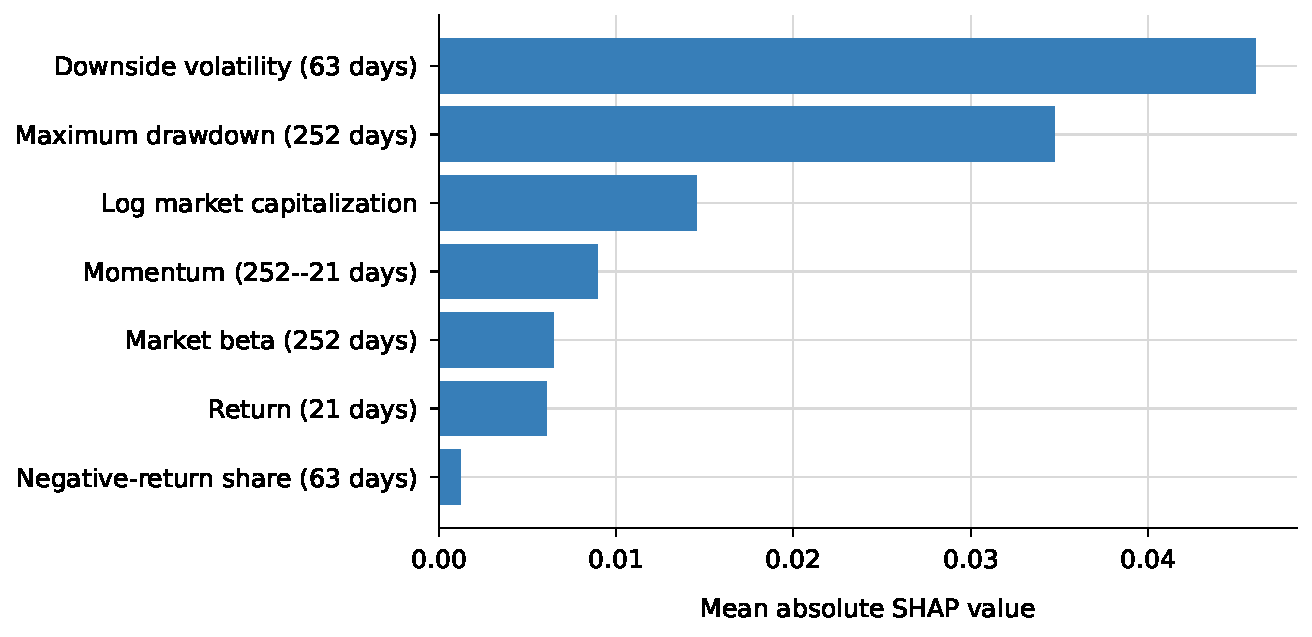
\includegraphics[width=\linewidth]{04_11_xgboost_global_shap_importance.pdf}
        \caption{Global importance.}
        \label{fig:selected-xgboost-shap-importance}
    \end{subfigure}
    \par\medskip
    \begin{subfigure}[t]{0.9\textwidth}
        \centering
        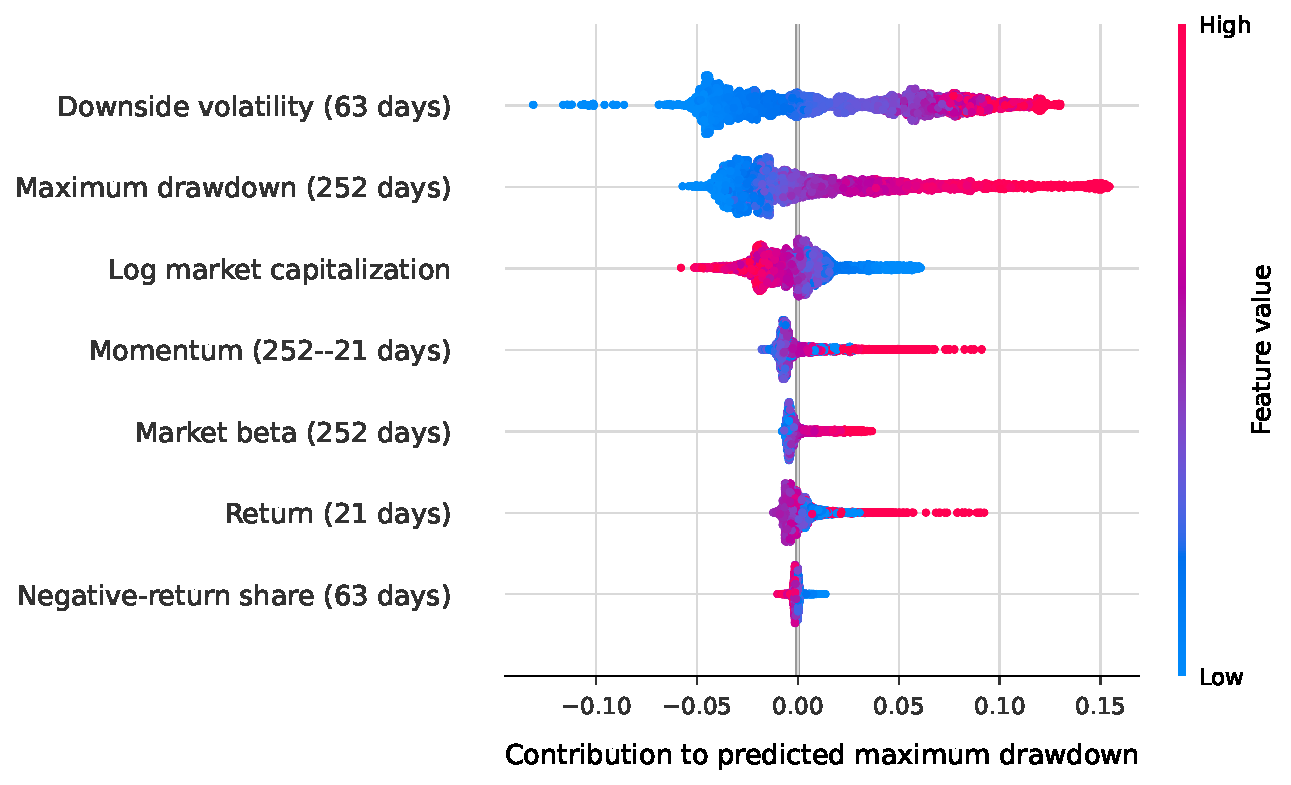
\includegraphics[width=\linewidth]{04_11_xgboost_shap_beeswarm.pdf}
        \caption{Direction and dispersion.}
        \label{fig:selected-xgboost-shap-beeswarm}
    \end{subfigure}
    \caption[SHAP interpretation of the selected XGBoost model]{Global SHAP importance and observation-level SHAP contributions for the selected market-only XGBoost model.}
    \label{fig:selected-xgboost-shap}
\end{figure}

\noindent
Higher downside volatility and larger past drawdowns generally increase predicted downside risk, whereas larger market capitalization generally reduces it. These relationships describe how the fitted model forms its predictions and should not be interpreted as causal effects. The dependence plots in Appendix~\ref{app:model_interpretation_details} provide the corresponding feature-level evidence. The same appendix shows that the ordering of feature importance remains stable across test quarters, indicating that the model does not rely on a different set of predictors in each period.

\subsection{Error Analysis}
\label{sec:selected_model_errors}

Building on the held-out evaluation in Section~\ref{sec:held_out_performance}, Figure~\ref{fig:selected-xgboost-error-diagnostics} examines where the selected model's errors occur. Predictions track the lower and middle realized-drawdown deciles reasonably well but increasingly understate losses in the upper tail. Consistent with this asymmetry, the signed-error distribution is concentrated near zero but has a pronounced positive tail, where realized drawdown exceeds the prediction.

\begin{figure}[!htbp]
    \centering
    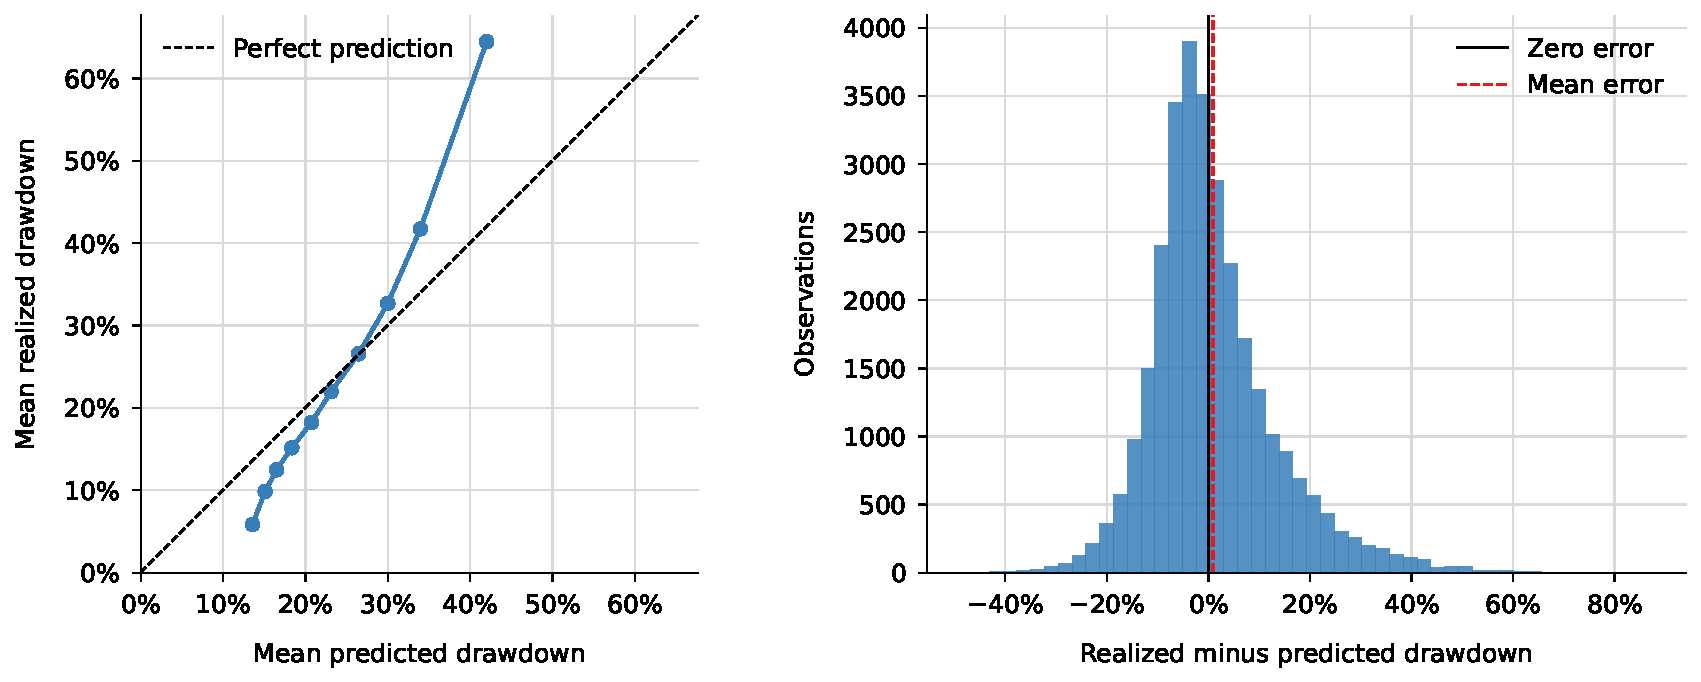
\includegraphics[width=0.95\textwidth]{04_09_xgboost_test_calibration_and_signed_errors.pdf}
    \caption[Calibration and signed errors of the selected model]{Mean predicted against realized drawdown across realized-drawdown deciles (left) and the distribution of realized-minus-predicted drawdown (right) in the held-out sample. Positive signed errors indicate that realized downside exceeded the prediction.}
    \label{fig:selected-xgboost-error-diagnostics}
\end{figure}

\noindent
As shown in Figure~\ref{fig:finalist-test-deciles} in Appendix~\ref{app:quarterly_test_performance}, MAE rises sharply in the most severe realized-drawdown decile. Supplementary quarterly and firm-size error diagnostics are reported in Appendices~\ref{app:quarterly_test_performance} and~\ref{app:firm_size_errors}.

Taken together, the diagnostics support using the predictions as a cross-sectional ranking of downside risk, but provide less support for interpreting individual forecasts as precisely calibrated estimates of extreme drawdown magnitudes.

\section{Predictive Robustness}
\label{sec:predictive_robustness_results}

The selected market-only XGBoost specification is re-estimated for the alternative downside outcomes defined in Section~\ref{sec:robustness}. Table~\ref{tab:predictive-robustness} reports held-out performance for downside volatility, the worst five-day loss, and maximum drawdown over 21 and 126 trading days, together with the primary 63-day target.

\begin{table}[!htbp]
\centering
\footnotesize
\caption{Held-out predictive robustness of the selected XGBoost specification.}
\label{tab:predictive-robustness}
\begin{tabular}{lrrrrrr}
\toprule
Target & Quarters & $\mathrm{MAE}$ & $\mathrm{RMSE}$ & $R^2$ & $\overline{\rho}$ & D10--D1 spread \\
\midrule
63-day maximum drawdown & 8 & 0.0912 & 0.1258 & 0.497 & 0.738 & 41.6\% \\
63-day downside volatility & 8 & 0.1211 & 0.2362 & 0.482 & 0.840 & 76.5\% \\
Worst five-day loss & 8 & 0.0594 & 0.0942 & 0.437 & 0.748 & 27.9\% \\
21-day maximum drawdown & 8 & 0.0627 & 0.0930 & 0.394 & 0.690 & 25.2\% \\
126-day maximum drawdown & 7 & 0.1113 & 0.1455 & 0.539 & 0.752 & 52.4\% \\
\bottomrule
\end{tabular}
\end{table}


\noindent
The absolute MAE values are not directly comparable because the targets have different scales. Rank correlations remain strong across all definitions, ranging from approximately 0.69 to 0.84. Positive Decile~10--Decile~1 spreads further indicate meaningful separation, including for the worst five-day loss and 21-day maximum drawdown. The strongest results occur for 63-day downside volatility, although its different scale and interpretation preclude direct comparison with drawdown outcomes. The predicted-risk decile profiles and quarterly diagnostics in Appendix~\ref{app:predictive_robustness_stability} show that ranking performance remains positive and comparatively stable across outcomes and individual test quarters. They also compare quarterly MAE with each target's overall test MAE, identifying relatively difficult quarters without making invalid comparisons between differently scaled outcomes.

The feature-importance comparison in Figure~\ref{fig:predictive-robustness-importance} further shows that recent downside volatility, past drawdown, and market capitalization remain the leading inputs across target definitions, although their relative weights change with the horizon and outcome.

\begin{figure}[!htbp]
    \centering
    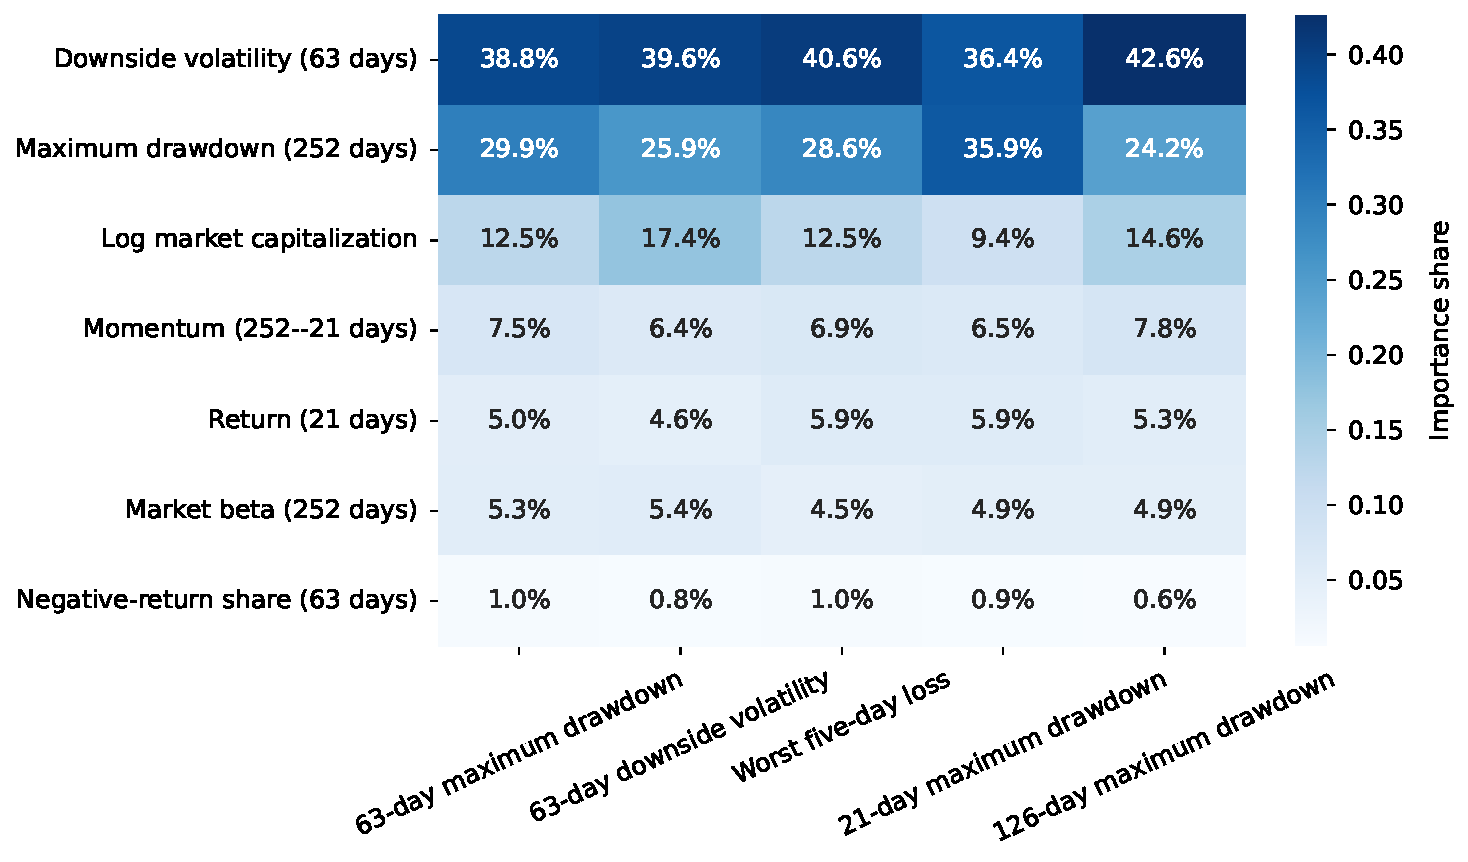
\includegraphics[width=0.88\textwidth]{04_10_xgboost_robustness_feature_importance_heatmap.pdf}
    \caption[Feature-importance stability across robustness targets]{SHAP importance shares across the primary and alternative downside-risk targets.}
    \label{fig:predictive-robustness-importance}
\end{figure}

\section{Fragility Score Evaluation}
\label{sec:fragility_statistical_evaluation}

The selected XGBoost predictions are converted into within-quarter percentile ranks, with higher Fragility Scores indicating greater predicted downside risk relative to other stocks in the same quarter. Table~\ref{tab:fragility-score-performance} summarizes the score's held-out ranking performance.

\begin{table}[!htbp]
\centering
\footnotesize
\caption{Held-out Fragility Score ranking performance.}
\label{tab:fragility-score-performance}
\begin{tabular}{lr}
\toprule
Statistic & Value \\
\midrule
Mean stock-level $\rho$: score vs. realized drawdown & 0.738 \\
Mean decile-level $\rho$: decile vs. realized drawdown & 1.000 \\
Mean realized-drawdown spread: Decile 10 minus Decile 1 & 41.6\% \\
\bottomrule
\end{tabular}
\end{table}


\noindent
At the stock level, the mean quarterly Spearman correlation between the Fragility Score and realized 63-day maximum drawdown is strong. At the decile level, mean realized drawdown increases monotonically with the Fragility Score in every test quarter, while the average realized-drawdown difference between Fragility Score Decile~10 and Decile~1 exceeds 40 percentage points. Figure~\ref{fig:fragility-score-deciles} and the supporting outcomes in Appendix~\ref{app:fragility_score_supporting_outcomes} show that higher score deciles also exhibit greater downside volatility, worse five-day losses, and weaker cumulative returns.

\section{Portfolio Evaluation}
\label{sec:portfolio_implications}

The portfolio analysis applies the Fragility Score using information available at each quarterly formation date. The primary equal-weighted comparison contrasts all eligible stocks with a portfolio excluding the most fragile decile. Decile~1 and Decile~10 serve as diagnostic portfolios showing the score's economic separation.

\subsection{Primary Long-Only Portfolios}
\label{sec:primary_portfolio_results}

Table~\ref{tab:portfolio-event-windows} summarizes the eight quarterly 63-day holding windows. Excluding Decile~10 reduces average maximum drawdown, downside volatility, and the worst five-day loss relative to the full equal-weighted universe. The contrast between Decile~1 and Decile~10 is substantially larger, confirming that the score separates stocks with very different subsequent downside outcomes. The corresponding graphical comparison is reported in Appendix~\ref{app:portfolio_window_risk}.

\begin{table}[!htbp]
\centering
\footnotesize
\caption{Mean performance across quarterly 63-day portfolio windows.}
\label{tab:portfolio-event-windows}
\begin{tabular}{lrrrr}
\toprule
Portfolio & Max. drawdown & Downside vol. & Worst 5-day loss & Cum. return \\
\midrule
All eligible stocks & 9.6\% & 13.5\% & 6.3\% & 3.2\% \\
Exclude Decile 10 & 8.6\% & 12.7\% & 5.7\% & 4.5\% \\
Decile 1 & 4.6\% & 6.9\% & 3.2\% & 2.2\% \\
Decile 10 & 24.4\% & 27.1\% & 13.6\% & -8.9\% \\
\bottomrule
\end{tabular}
\end{table}


\noindent
The continuous-strategy results in Table~\ref{tab:portfolio-performance} and Figure~\ref{fig:portfolio-strategy-wealth} point in the same direction. The screened portfolio improves on the matched equal-weighted universe in return, volatility, Sharpe ratio, and maximum drawdown. It nevertheless underperforms the external CRSP total-market benchmark, which has both higher returns and a better downside profile over the same period.

\begin{table}[!htbp]
\centering
\footnotesize
\caption{Continuous Fragility Score portfolio performance.}
\label{tab:portfolio-performance}
\begin{tabular}{lrrrrr}
\toprule
Strategy & Cum. return & Ann. return & Ann. vol. & Sharpe & Max. drawdown \\
\midrule
All eligible stocks & 16.2\% & 7.8\% & 20.4\% & 0.24 & 26.5\% \\
Exclude Decile 10 & 29.5\% & 13.8\% & 19.5\% & 0.52 & 24.1\% \\
CRSP total market & 41.4\% & 19.0\% & 16.4\% & 0.85 & 19.1\% \\
\bottomrule
\end{tabular}
\end{table}


\begin{figure}[!htbp]
    \centering
    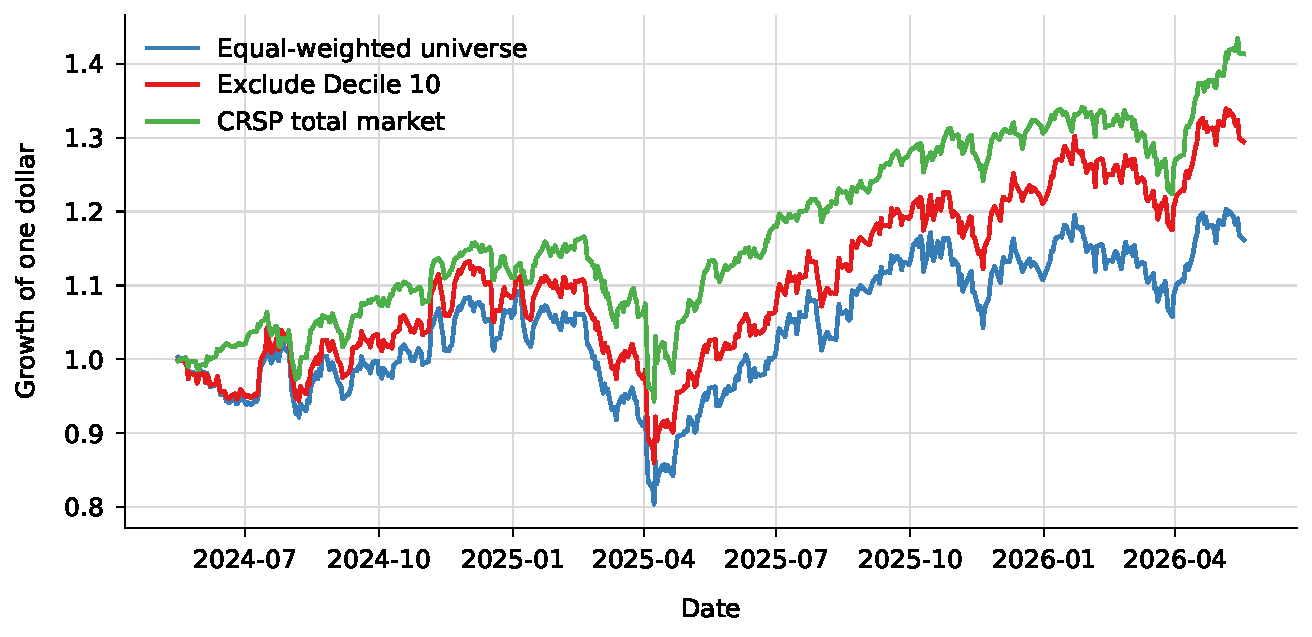
\includegraphics[width=0.82\textwidth]{04_11_fragility_strategy_wealth.pdf}
    \caption[Cumulative wealth of the primary portfolio strategies]{Cumulative wealth of the full equal-weighted universe, the portfolio excluding Decile~10, and the CRSP total-market index.}
    \label{fig:portfolio-strategy-wealth}
\end{figure}

\noindent
Figure~\ref{fig:portfolio-strategy-alpha} presents the factor-adjusted evidence. The screened portfolio has approximately zero FF5-plus-momentum alpha, whereas the screened-minus-unscreened portfolio has a positive alpha whose 95\% confidence interval excludes zero. This indicates a benefit relative to the matched internal universe, not superiority to the broad market. Complete regression statistics appear in Appendix~\ref{app:primary_portfolio_alpha}.

\begin{figure}[!htbp]
    \centering
    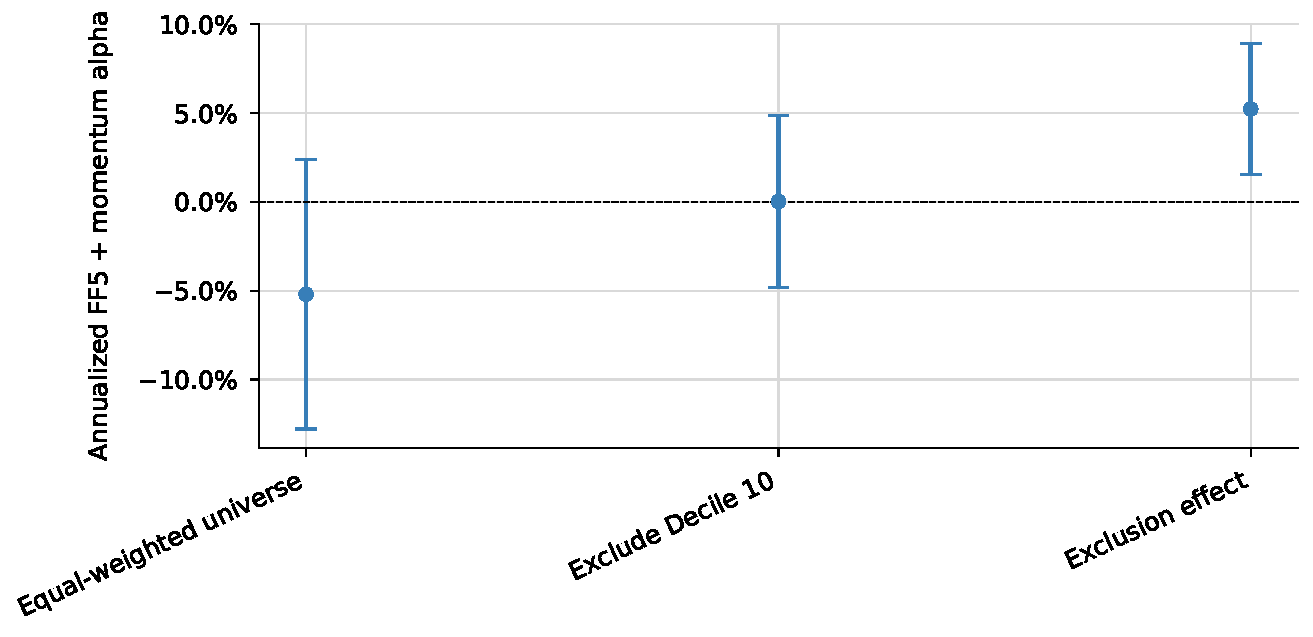
\includegraphics[width=0.76\textwidth]{04_11_fragility_strategy_alpha.pdf}
    \caption[Factor-adjusted alpha of the primary portfolios]{Annualized FF5-plus-momentum alpha with 95\% confidence intervals for the full, screened, and screened-minus-full portfolios.}
    \label{fig:portfolio-strategy-alpha}
\end{figure}

\subsection{Long-Only Portfolio Robustness}
\label{sec:portfolio_robustness_results}

The long-only robustness analysis tests sensitivity to the exclusion threshold and weighting rule. Table~\ref{tab:portfolio-robustness} shows that excluding the top 20\% produces results similar to excluding Decile~10 under equal weighting. Under value weighting, however, excluding Decile~10 has almost no effect. The score's benefit is therefore concentrated among smaller stocks and depends on the weighting rule, consistent with the firm-size error pattern in Section~\ref{sec:selected_model_errors}. A graphical comparison appears in Appendix~\ref{app:portfolio_robustness_figure}.

\begin{table}[!htbp]
\centering
\footnotesize
\caption{Long-only portfolio robustness results.}
\label{tab:portfolio-robustness}
\begin{tabular}{lrrrr}
\toprule
Strategy & Ann. return & Ann. vol. & Sharpe & Max. drawdown \\
\midrule
Equal weight: all stocks & 7.8\% & 20.4\% & 0.24 & 26.5\% \\
Equal weight: exclude Decile 10 & 13.8\% & 19.5\% & 0.52 & 24.1\% \\
Equal weight: exclude top 20\% & 13.4\% & 18.5\% & 0.51 & 23.4\% \\
Value weight: all stocks & 19.3\% & 16.6\% & 0.86 & 19.4\% \\
Value weight: exclude Decile 10 & 19.2\% & 16.6\% & 0.86 & 19.4\% \\
\bottomrule
\end{tabular}
\end{table}


\FloatBarrier

\subsection{Long--Short Extensions}
\label{sec:long_short_results}

The long--short analysis examines the return spread between the least- and most-fragile stocks. DFRAG-10 uses the extreme deciles, DFRAG-20 uses the two lowest and highest deciles, and volatility-managed DFRAG-10 scales exposure using lagged realized volatility. Table~\ref{tab:long-short-performance} and Figure~\ref{fig:long-short-wealth} compare the three specifications. DFRAG-10 produces the highest return but is volatile and concentrated, whereas volatility management reduces volatility and maximum drawdown while retaining positive returns.

\begin{table}[!htbp]
\centering
\footnotesize
\caption{Exploratory long--short Fragility Score strategies.}
\label{tab:long-short-performance}
\begin{tabular}{lrrrr}
\toprule
Strategy & Ann. return & Ann. volatility & Sharpe & Max. drawdown \\
\midrule
DFRAG-10 & 55.7\% & 34.6\% & 1.45 & 41.4\% \\
DFRAG-20 & 16.0\% & 29.6\% & 0.65 & 42.5\% \\
DFRAG-10: volatility managed & 28.2\% & 17.3\% & 1.52 & 21.1\% \\
\bottomrule
\end{tabular}
\end{table}


\begin{figure}[H]
    \centering
    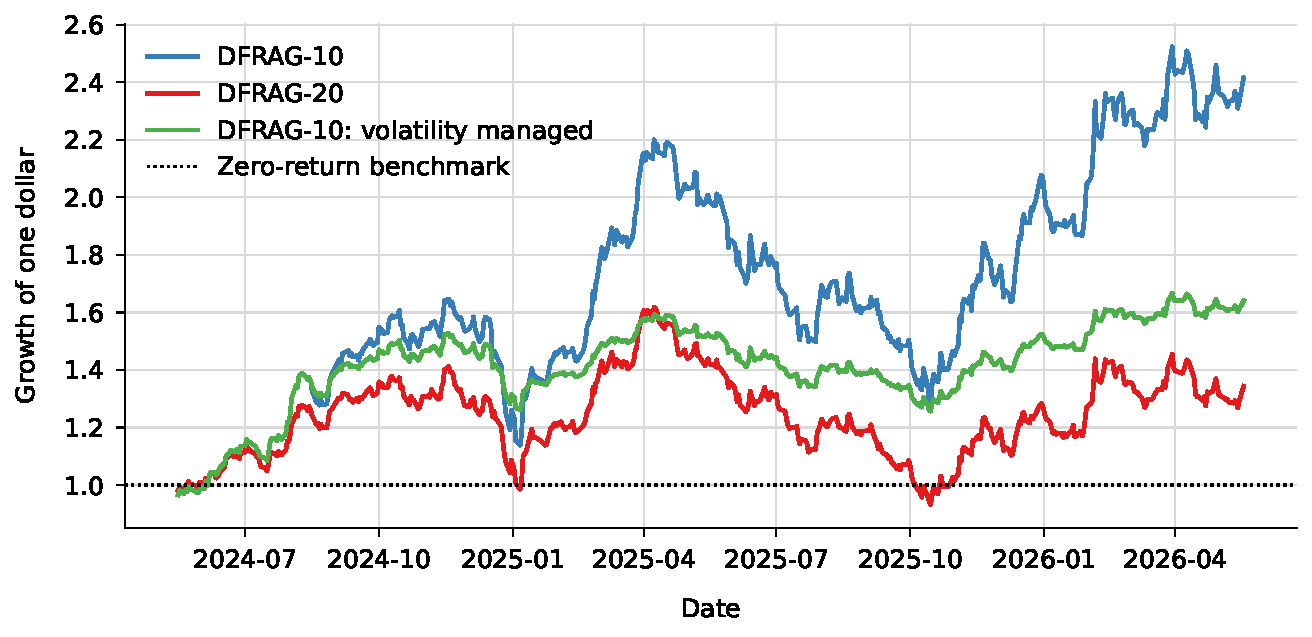
\includegraphics[width=0.76\textwidth]{04_12_long_short_fragility_wealth.pdf}
    \caption[Cumulative wealth of the exploratory long--short strategies]{Cumulative wealth of DFRAG-10, DFRAG-20, and volatility-managed DFRAG-10. The horizontal line at one denotes zero return.}
    \label{fig:long-short-wealth}
\end{figure}

\noindent
The FF5-plus-momentum alpha estimate for DFRAG-10 is positive and its 95\% confidence interval excludes zero, whereas the DFRAG-20 and volatility-managed estimates are less precise. These estimates are shown in Figure~\ref{fig:long-short-alpha}. They should nevertheless be interpreted cautiously because the evaluation period is short and the strategies require substantial short-side implementation.

\begin{figure}[!htbp]
    \centering
    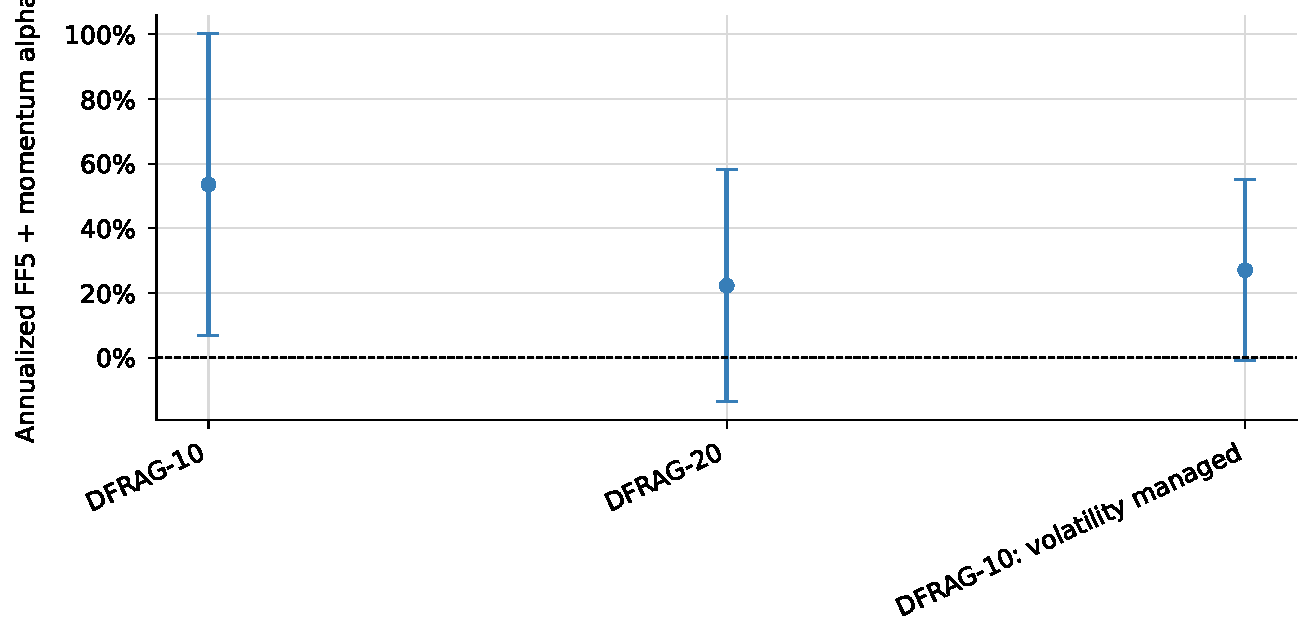
\includegraphics[width=0.76\textwidth]{04_12_long_short_fragility_alpha.pdf}
    \caption[Factor-adjusted alpha of the exploratory long--short strategies]{Annualized FF5-plus-momentum alpha with 95\% confidence intervals for DFRAG-10, DFRAG-20, and volatility-managed DFRAG-10.}
    \label{fig:long-short-alpha}
\end{figure}

\noindent
Table~\ref{tab:long-short-implementation} makes this limitation explicit. Average one-way turnover is high, particularly for volatility-managed DFRAG-10. Applying a 50-basis-point one-way trading cost reduces performance but does not eliminate the gross return in this short sample. The corresponding results under 10-, 25-, and 50-basis-point assumptions are reported in Appendix~\ref{app:long_short_cost_sensitivity}. These calculations still omit several material frictions, including borrowing availability, stock-loan fees, and market impact. The long--short evidence is therefore exploratory and does not support a tradable-factor interpretation.

\begin{table}[!htbp]
\centering
\footnotesize
\caption{Mean one-way turnover and annualized gross and net returns of the long--short strategies.}
\label{tab:long-short-implementation}
\begin{tabular}{lrrr}
\toprule
Strategy & Mean turnover & Gross return & Net return (50 bps) \\
\midrule
DFRAG-10 & 96.2\% & 55.7\% & 52.7\% \\
DFRAG-20 & 83.3\% & 16.0\% & 14.0\% \\
DFRAG-10: volatility managed & 130.7\% & 28.2\% & 24.9\% \\
\bottomrule
\end{tabular}
\end{table}


\noindent
Overall, the Fragility Score has clear economic ordering power and modestly improves the downside profile of the matched equal-weighted portfolio. Its portfolio value is qualified by weighting sensitivity, implementation costs, and the stronger performance of the external market benchmark.

\section{Summary of Evidence}
\label{sec:results_summary}

Table~\ref{tab:hypothesis-summary} summarizes the empirical conclusions. Conventional ownership variables provide only a small validation improvement, while engineered network features do not add a consistent incremental gain. XGBoost modestly improves on Ridge using the same market information. Temporal GraphSAGE is competitive and records the lowest validation and test MAE, but it does not dominate the simpler tabular model across metrics and therefore provides no decisive support for the additional graph-learning complexity.

\begin{table}[!htbp]
\centering
\footnotesize
\caption{Summary of evidence for the research hypotheses.}
\label{tab:hypothesis-summary}
\begin{tabular}{lp{0.58\textwidth}l}
\toprule
Hypothesis & Evidence & Assessment \\
\midrule
H1 & Ownership features produce only small validation improvements. & Limited support \\
H2 & Engineered network features add no consistent incremental gain. & Not supported \\
H3 & XGBoost modestly improves on Ridge with identical market inputs. & Moderate support \\
H4 & Temporal GraphSAGE is competitive, but not consistently superior across metrics. & Mixed evidence \\
H5 & The score strongly ranks downside risk; portfolio evidence is positive but qualified. & Qualified support \\
\bottomrule
\end{tabular}
\end{table}


\noindent
The clearest result concerns the final prediction. The selected market-only XGBoost model produces a strong and stable ranking of subsequent downside risk. The resulting Fragility Score separates realized maximum drawdown monotonically and produces consistent risk gradients across alternative downside outcomes. Portfolio applications preserve part of this ordering: excluding the most fragile stocks improves the matched equal-weighted portfolio, while the exploratory long--short signal is economically large within the short evaluation period. These findings remain sensitive to weighting and implementation assumptions, and the screened portfolio does not outperform the broad market. Hypothesis~H5 therefore receives qualified support, while the central practical contribution is the score's forward-looking risk ranking rather than a directly deployable investment strategy.


\chapter{Conclusion}
\label{chap:conclusion}

This chapter answers the research question in light of the empirical evidence, summarizes the thesis's contributions, and sets out its limitations. Particular emphasis is placed on the distinction between the strong evidence for the Fragility Score as a downside-risk ranking and the more conditional evidence from its portfolio applications. The chapter closes by identifying the extensions needed to assess the score over longer periods and under more realistic implementation conditions.

\section{Answer to the Research Question}
\label{sec:conclusion_summary}

This thesis asked whether conventional institutional ownership measures and the topology of institutional ownership improve the out-of-sample prediction of stock-level downside risk beyond market characteristics, whether graph-based models exploit that structure more effectively than comparable tabular models, and whether the resulting predictions have economic value. The answer is qualified. Conventional ownership measures contain limited incremental information, but neither the engineered network features nor direct graph learning provide a consistent advantage sufficient to justify their additional complexity. The strongest result is instead that the selected model's predictions provide an informative out-of-sample ranking of subsequent downside risk.

The empirical design separates information, model flexibility, and evaluation timing. Quarterly Form 13F holdings are aligned with CRSP market data using a common information cutoff, and the primary outcome is the positive magnitude of maximum drawdown over the following 63 trading days. Market, ownership, and engineered network features form nested information sets evaluated using Ridge and XGBoost, while three graph neural networks learn directly from the manager--stock graph. Feature selection, preprocessing, tuning, and model comparison use chronological training and validation samples separated from the 2024~Q1--2025~Q4 test period by purged quarters. The test sample is examined only after the model-selection decision is fixed.

The feature comparisons provide limited support for Hypothesis~H1: ownership variables produce small validation improvements, but not enough to displace the market-only specification under the stated parsimony rule. Engineered network features add no consistent improvement, so Hypothesis~H2 is not supported. Market-only XGBoost modestly outperforms market-only Ridge on validation and test data, supporting Hypothesis~H3. At the validation stage, Temporal GraphSAGE has the lowest MAE, whereas XGBoost has better RMSE and $R^2$ and essentially identical ranking performance. Market-only XGBoost is therefore selected as the performance--parsimony choice before the test sample is examined. The held-out comparison preserves this pattern: Temporal GraphSAGE has the lowest MAE, while XGBoost has better RMSE and $R^2$ and nearly identical ranking performance. The graph evidence is competitive but not consistently superior, giving mixed support to Hypothesis~H4.

On the held-out sample, the selected XGBoost model achieves an MAE of 0.0912, an $R^2$ of 0.497, and a mean quarterly Spearman correlation of 0.738. Mean realized maximum drawdown increases monotonically across Fragility Score deciles in every test quarter, and the average Decile~10--Decile~1 spread is 41.6 percentage points. Positive rank correlations and decile spreads across the alternative targets show that the ranking extends beyond the primary 63-day drawdown definition. The error analysis nevertheless shows that forecasts understate some of the most severe realized losses. The score is therefore better supported as a relative measure of downside exposure than as a precisely calibrated forecast of extreme drawdown magnitude.

The portfolio evidence is more conditional. Excluding the most fragile decile improves the downside profile of the matched equal-weighted universe, and the screened-minus-unscreened return difference has a positive FF5-plus-momentum alpha. The screened portfolio itself has approximately zero alpha, does not outperform the external CRSP total-market benchmark, and provides almost no improvement under value weighting. The exploratory long--short portfolios further separate low- and high-score stocks, but the short evaluation period, substantial turnover, large drawdowns, and incomplete treatment of short-side costs do not support a tradable-factor interpretation. Hypothesis~H5 consequently receives qualified support. The most defensible application of the Fragility Score is risk monitoring and portfolio screening, particularly within a specified investment universe, rather than return forecasting or stand-alone trading.

\section{Contributions and Implications}
\label{sec:contributions}

The thesis makes three related contributions. Empirically, it tests the incremental predictive content of conventional ownership measures and ownership-network topology for a forward stock-level downside outcome. This extends the ownership-fragility literature, which links ownership structure and crowding to volatility and drawdowns, by evaluating the information through a fixed out-of-sample forecasting design \parencite{greenwood2011stock,brown2022crowded}. The results distinguish limited information in conventional ownership variables from the absence of a reliable incremental gain from the network representations tested here. This conclusion is specific to the variables, graph construction, models, and sample used in the thesis; it does not imply that institutional ownership or financial networks are generally uninformative.

Methodologically, the tabular comparisons change one dimension at a time. Ridge and XGBoost are compared on matched information sets, and graph models are evaluated separately as a method for learning directly from ownership relations. Point-in-time feature construction, purged chronological boundaries, fitting-sample preprocessing, and validation-stage model selection preserve the sequence in which information would have become available. The selected specification is fixed before the test sample is examined, and the held-out comparison is used to assess generalization rather than to reopen selection. This design makes it possible to distinguish small predictive gains from the effects of additional inputs or model complexity.

Economically, the thesis converts predicted drawdown into a Fragility Score computed within each quarter and evaluates it sequentially as a risk ranking, a long-only exclusion screen, and an exploratory long--short signal. The evidence is strongest at the first stage: the score consistently orders subsequent downside outcomes. Its long-only benefit is visible in the equal-weighted universe but nearly disappears under value weighting, while the long--short results depend on a short sample and simplified implementation assumptions. The appropriate implication is therefore narrower than a trading claim. The score may support risk monitoring, security review, or exclusion-based screening within a defined universe; the thesis does not establish that it should determine portfolio weights or serve as a stand-alone return signal.

\section{Limitations}
\label{sec:limitations}

The results should be interpreted within four boundaries. First, the held-out evaluation contains 30,511 stock-quarter observations but only eight formation quarters from 2024~Q1 through 2025~Q4 and 502 trading days in the continuous portfolio analysis. The cross-section is therefore large relative to the time dimension. Chronological separation protects the reported test from model selection, but a single short test period cannot establish stability across market regimes.

Second, Form 13F is a partial and delayed representation of institutional portfolios. It reports specified positions quarterly for managers meeting the regulatory threshold \parencite{sec2023form13f}; it does not reveal the complete investor base, short positions, or trading between reporting dates. The ownership and network variables consequently measure reported institutional long-equity exposure available at the common information cutoff, not the full set of positions or the trading process that generated them. The analysis is predictive, and neither the fitted relationships nor the SHAP diagnostics identify causal effects of ownership structure on later drawdowns.

Third, the model comparisons are conditional on the implemented specifications and search ranges. Ridge uses the prespecified penalty $\alpha=1$, whereas XGBoost and the selected graph architecture undergo controlled validation refinements. Ridge and XGBoost minimize squared-error objectives, while the graph models use $L_1$ loss. Hypotheses~H3 and~H4 should therefore be interpreted as comparisons among the implemented specifications rather than exhaustive comparisons among optimally tuned model classes. Manager similarity is represented through a 25-nearest-neighbour graph, Louvain communities are estimated separately each quarter, and the tabular models receive the network features retained by the prespecified redundancy screen. The graph comparison covers weighted GraphSAGE, GAT, and Temporal GraphSAGE under a bounded tuning exercise. The absence of consistent incremental performance applies to these representations; it does not rule out alternative edge definitions, community methods, temporal structures, or graph architectures. The comparisons are also based on point estimates rather than formal tests of differences in predictive accuracy. Given the small gaps among the finalists and the limited time dimension described above, the evidence does not establish that these differences are statistically distinguishable; a longer test period and inference that accounts for cross-sectional and temporal dependence would strengthen the comparison. In addition, each graph architecture is estimated using a single fixed random seed, so sensitivity to random initialization is not measured. These qualifications do not change the validation-stage selection decision: XGBoost is retained because it combines similar MAE and ranking performance with stronger RMSE and $R^2$ and substantially lower complexity, rather than because it achieves the lowest MAE. The similar metric pattern observed in validation and test provides some cross-period reassurance, but it does not resolve the inferential or seed-related uncertainty.

Fourth, the portfolio tests do not constitute a complete implementation study. The strongest long-only result is obtained under equal weighting and becomes negligible under value weighting, indicating sensitivity to the weighting rule and the influence of smaller stocks. The CRSP total-market index is an external reference rather than a matched benchmark. Transaction costs are modeled through fixed turnover-based assumptions, while market impact, capacity, taxes, stock-borrow availability, borrowing fees, and financing costs are not fully incorporated. The long--short and volatility-managed results should therefore be interpreted as evidence of economic separation, not as verified net-of-cost investment performance.

\section{Future Research}
\label{sec:future_research}

The first priority for future research is a longer walk-forward evaluation with repeated validation and test windows. More formation periods would permit a stronger assessment of whether the downside-risk ranking, the small ownership-feature gains, and the equal-weight screening result persist across different market conditions. Statistical inference for the portfolio applications would also benefit from a longer return history.

A second extension is to vary the representation of ownership topology while preserving the controlled comparison used in this thesis. Alternative manager-similarity rules, edge definitions, community methods, temporal architectures, and graphs with multiple relation types could capture information omitted by the present construction. Such models should be compared with the same market-only and ownership-based alternatives so that any improvement can be attributed to the added relational information rather than to a broader tuning search.

The prediction task could also be adapted to the limitation identified by the error analysis. Quantile objectives, tail-weighted losses, or classification of drawdowns above a prespecified threshold could focus directly on severe events that the current point forecasts tend to understate. For economic evaluation, future work should use matched investable benchmarks, capacity-aware portfolio construction, and direct estimates of trading, financing, and stock-borrow costs. The near-disappearance of the screening effect under value weighting also warrants explicit analysis of firm size and liquidity before any investment interpretation is advanced.

Overall, the thesis finds that stock-level downside risk can be ranked meaningfully out of sample using information available at the prediction date. Conventional ownership variables add only limited incremental information, and the tested network features and graph models do not deliver a consistent advantage sufficient to justify their complexity. The Fragility Score is therefore best interpreted as a risk-monitoring and portfolio-screening device whose portfolio relevance remains conditional on the investment universe, weighting rule, evaluation period, and implementation assumptions. Stronger claims about trading performance require longer evidence and a more complete treatment of investability and costs.


% ==================================================
% BIBLIOGRAPHY
% ==================================================

\clearpage
\printbibliography[
    heading=bibintoc,
    title={References}
]

% ==================================================
% APPENDICES
% ==================================================

\appendix
\chapter{Methodological Details}
\label{chap:methodology_appendix}
This appendix provides supplementary construction details and diagnostics for the methodology developed in Chapter~\ref{chap:methodology}. It documents the sample-construction procedures, feature definitions and diagnostics, preprocessing and selection rules, chronological sample allocation, and predictive-model specifications. The material supports the reproducibility of the empirical design while keeping the main chapter focused on its essential methodological choices.

\section{Sample Construction}
\label{app:sample_construction}

Filing selection is performed separately for each manager and reporting quarter. The SEC distinguishes holdings reports from notice reports through the EDGAR submission type and the cover-page report type \parencite[FAQs 20 and 33]{sec2023form13f}. For this analysis, a filing is eligible only if it was submitted by the common information cutoff and both classifications identify it as a holdings report. Notice filings, filings with conflicting classifications, and filings submitted after the cutoff are excluded. Among the remaining original filings and restatements, the base filing is selected by ordering candidates by amendment number, filing date, and accession number and retaining the final observation. Earlier bases are treated as superseded. A later amendment is retained as an addition only when its amendment number is greater than that of the selected base. This rule produces one reproducible set of filings for each eligible manager-quarter while using only information available by the prediction date.

For security mapping, nine-character CUSIPs are normalized and matched exactly to CRSP CUSIP histories whose validity intervals contain the relevant reporting date. A position is classified as matched only when this procedure identifies one unique PERMNO; observations with no candidate or multiple candidates are classified as unmatched or ambiguous, respectively. The holdings panel subsequently retains matched securities classified by CRSP as common equity and aggregates their reported positions first at the manager-security level and then into stock-quarter ownership measures.

Table~\ref{tab:sample_construction} summarizes the construction of the final modeling sample. Observations that lack either usable historical market features or a usable forward target remain in the full panel with explicit eligibility flags rather than being deleted. Overall, approximately 184,000 observations, or 89\% of the full panel, enter the three modeling samples, indicating that the eligibility and purging rules preserve broad coverage while enforcing the point-in-time design.

\begin{table}[H]
    \centering
    \caption{Stock-quarter panel and modeling-sample construction}
    \label{tab:sample_construction}
    \begin{tabular}{lr}
        \toprule
        Characteristic & Value \\
        \midrule
        Coverage & 2013 Q2--2026 Q1 \\
        Reporting quarters & 52 \\
        Distinct securities & 7,232 \\
        Full stock-quarter observations & 206,868 \\
        Usable predictors and target & 192,109 (92.87\%) \\
        Final modeling observations & 184,018 (88.95\%) \\
        \bottomrule
    \end{tabular}
\end{table}


\section{Downside-Risk Target Statistics}
\label{app:target_statistics}

Table~\ref{tab:target_statistics} summarizes the distributions of the primary 63-day maximum-drawdown target and the four alternative downside-risk definitions used in the robustness analysis. Statistics are calculated over usable observations from the common modeling universe, applying the corresponding usability rule to each target. All distributional statistics except skewness are reported as percentages.

\begin{table}[!htbp]
    \centering
    \scriptsize
    \setlength{\tabcolsep}{4pt}
    \caption{Distributional statistics for downside-risk targets}
    \label{tab:target_statistics}
    \begin{tabular}{lrrrrrrrr}
        \toprule
        Target definition & Mean & SD & P1 & P10 & Median & P90 & P99 & Skewness \\
        \midrule
        63-day maximum drawdown & 21.52\% & 16.22\% & 0.98\% & 6.24\% & 16.73\% & 44.20\% & 77.41\% & 1.52 \\
        63-day downside volatility & 33.62\% & 27.61\% & 2.58\% & 12.34\% & 25.92\% & 63.08\% & 132.38\% & 5.74 \\
        63-day worst five-day loss & 13.65\% & 10.97\% & 0.60\% & 4.39\% & 10.54\% & 26.48\% & 57.83\% & 2.38 \\
        21-day maximum drawdown & 12.03\% & 11.15\% & 0.55\% & 2.89\% & 8.50\% & 25.66\% & 55.71\% & 2.33 \\
        126-day maximum drawdown & 29.64\% & 20.06\% & 1.42\% & 9.31\% & 24.01\% & 59.44\% & 89.08\% & 1.07 \\
        \bottomrule
    \end{tabular}
\end{table}


\section{Market Feature Definitions and Diagnostics}
\label{app:market_features}

Table~\ref{tab:market-feature-definitions} gives the exact construction of the nine market predictors. Let $t$ denote the final trading day strictly before the information cutoff, $D_k$ the $k$ trading days ending on $t$, $r_{i,d}$ the daily return of stock $i$, and $r_{M,d}$ the CRSP total-market return. The complete feature window contains the final 252 trading days before the cutoff. Only regular-way observations with an active trading-status flag enter the calculations.

\begingroup
\scriptsize
\setlength{\tabcolsep}{4pt}
\renewcommand{\arraystretch}{1.15}
\begin{longtable}{>{\raggedright\arraybackslash}p{0.22\textwidth}>{\raggedright\arraybackslash}p{0.48\textwidth}>{\raggedright\arraybackslash}p{0.20\textwidth}}
        \caption{Exact definitions of the market predictors}
        \label{tab:market-feature-definitions}                                                                                                                                                                         \\
        \toprule
        Feature & Exact construction                                                                                                                                                         & Window and requirements \\
        \midrule
        \endfirsthead
        \toprule
        Feature & Exact construction                                                                                                                                                         & Window and requirements \\
        \midrule
        \endhead
        \bottomrule
        \endfoot
        \nolinkurl{market_cap_usd}
                & Most recent eligible CRSP daily market capitalization observed before the cutoff; the CRSP value is multiplied by 1,000 to express it in U.S. dollars.
                & Latest observation in the 252-day window.                                                                                                                                                            \\
        \nolinkurl{average_daily_dollar_volume_63d}
                & $|D_{63}|^{-1}\sum_{d\in D_{63}}|P_{i,d}|V_{i,d}$, where $P_{i,d}$ and $V_{i,d}$ are the CRSP daily price and volume.
                & 63 trading days.                                                                                                                                                                                     \\
        \nolinkurl{return_21d}
                & $\prod_{d\in D_{21}}(1+r_{i,d})-1$.
                & 21 trading days.                                                                                                                                                                                     \\
        \nolinkurl{momentum_252_21d}
                & Cumulative return from the beginning of the 252-day feature window through the day immediately preceding the final 21 trading days: $\prod_{d=t-251}^{t-21}(1+r_{i,d})-1$.
                & 231 trading days, with the most recent 21 days omitted.                                                                                                                                              \\
        \nolinkurl{volatility_63d}
                & Sample standard deviation of $r_{i,d}$ multiplied by $\sqrt{252}$.
                & 63 trading days; annualized.                                                                                                                                                                         \\
        \nolinkurl{downside_volatility_63d}
                & $\sqrt{252\,|D_{63}|^{-1}\sum_{d\in D_{63}}\min(r_{i,d},0)^2}$.
                & 63 trading days; annualized around a zero-return threshold.                                                                                                                                          \\
        \nolinkurl{market_beta_252d}
                & Ordinary-least-squares slope from regressing $r_{i,d}$ on the contemporaneous CRSP total-market return $r_{M,d}$.
                & 252 trading days; at least 202 paired observations.                                                                                                                                                  \\
        \nolinkurl{maximum_drawdown_252d}
                & Positive magnitude of the largest peak-to-trough decline in cumulative stock wealth, calculated by the same convention as the forward target.
                & 252 trading days.                                                                                                                                                                                    \\
        \nolinkurl{negative_return_share_63d}
                & $|D_{63}|^{-1}\sum_{d\in D_{63}}\mathbf{1}\{r_{i,d}<0\}$.
                & 63 trading days.                                                                                                                                                                                     \\
\end{longtable}
\endgroup

\noindent
A stock-quarter's market features are considered usable only when the 63-day window contains at least 50 observed returns, the 252-day window contains at least 202 observed returns, beta has at least 202 paired stock-market observations, and the latest price and market capitalization are positive. Figure~\ref{fig:market-feature-distributions} summarizes the training-sample distributions of the nine market predictors, with values clipped at their 1st and 99th percentiles for display only.

\begin{figure}[H]
        \centering
        \begin{subfigure}[t]{0.31\textwidth}
                \centering
                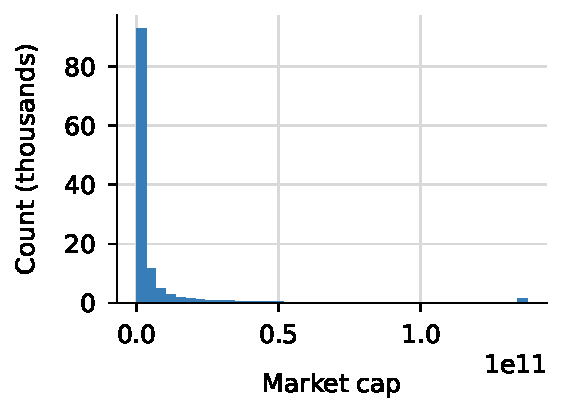
\includegraphics[width=\linewidth]{04_00_market_feature_distribution_01_market_cap_usd.pdf}
        \end{subfigure}
        \hfill
        \begin{subfigure}[t]{0.31\textwidth}
                \centering
                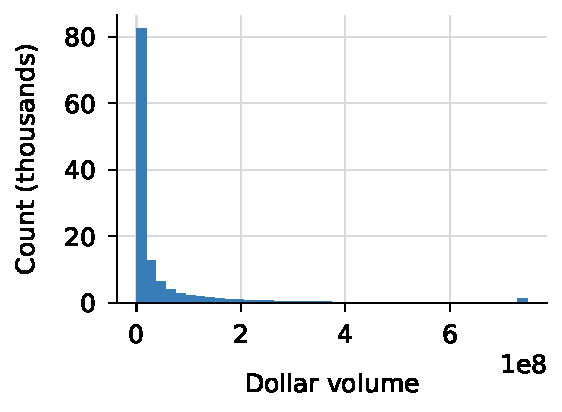
\includegraphics[width=\linewidth]{04_00_market_feature_distribution_02_average_daily_dollar_volume_63d.pdf}
        \end{subfigure}
        \hfill
        \begin{subfigure}[t]{0.31\textwidth}
                \centering
                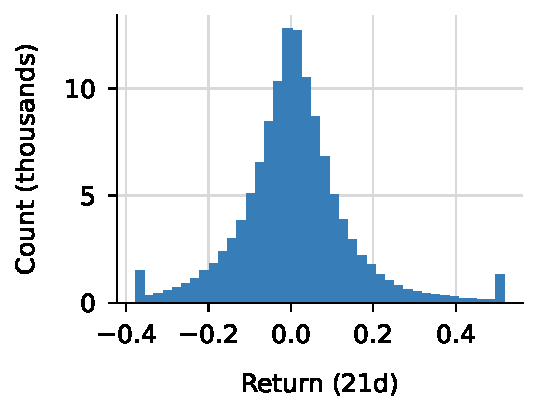
\includegraphics[width=\linewidth]{04_00_market_feature_distribution_03_return_21d.pdf}
        \end{subfigure}
        \par\medskip
        \begin{subfigure}[t]{0.31\textwidth}
                \centering
                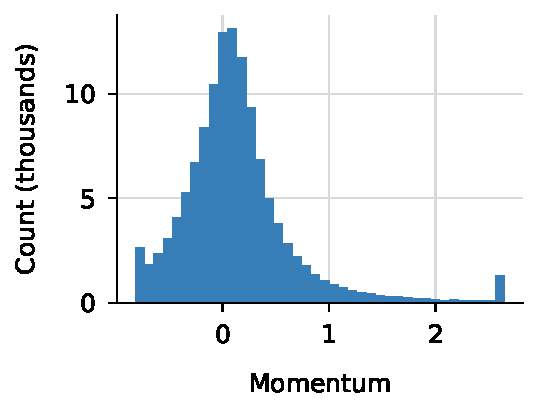
\includegraphics[width=\linewidth]{04_00_market_feature_distribution_04_momentum_252_21d.pdf}
        \end{subfigure}
        \hfill
        \begin{subfigure}[t]{0.31\textwidth}
                \centering
                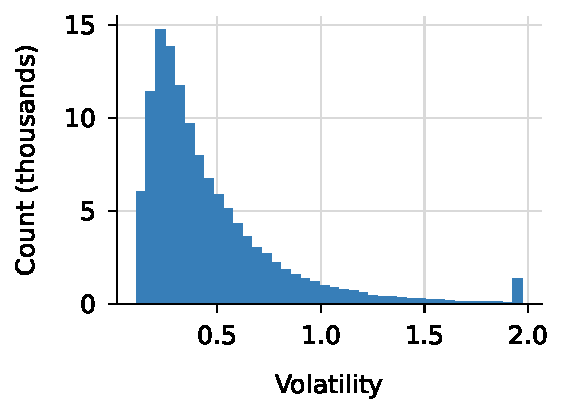
\includegraphics[width=\linewidth]{04_00_market_feature_distribution_05_volatility_63d.pdf}
        \end{subfigure}
        \hfill
        \begin{subfigure}[t]{0.31\textwidth}
                \centering
                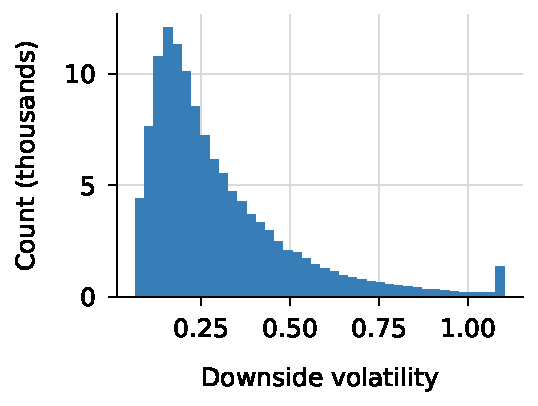
\includegraphics[width=\linewidth]{04_00_market_feature_distribution_06_downside_volatility_63d.pdf}
        \end{subfigure}
        \par\medskip
        \begin{subfigure}[t]{0.31\textwidth}
                \centering
                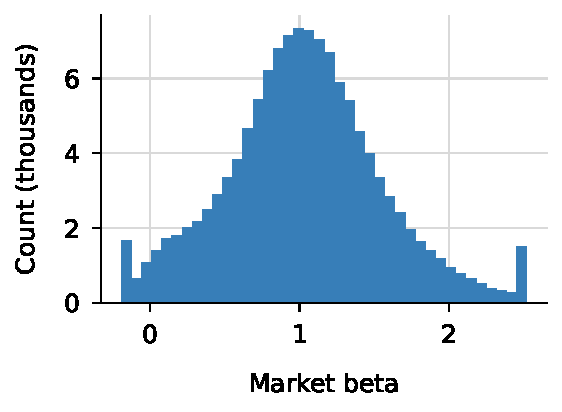
\includegraphics[width=\linewidth]{04_00_market_feature_distribution_07_market_beta_252d.pdf}
        \end{subfigure}
        \hfill
        \begin{subfigure}[t]{0.31\textwidth}
                \centering
                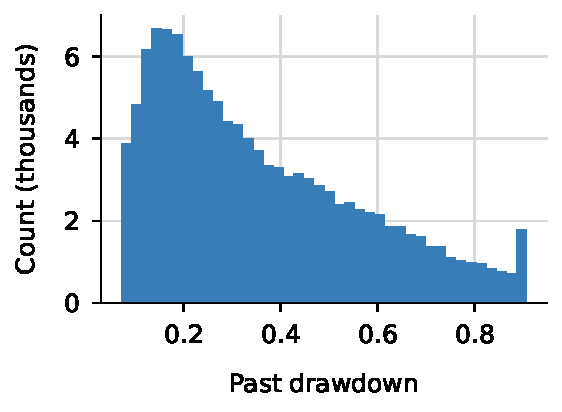
\includegraphics[width=\linewidth]{04_00_market_feature_distribution_08_maximum_drawdown_252d.pdf}
        \end{subfigure}
        \hfill
        \begin{subfigure}[t]{0.31\textwidth}
                \centering
                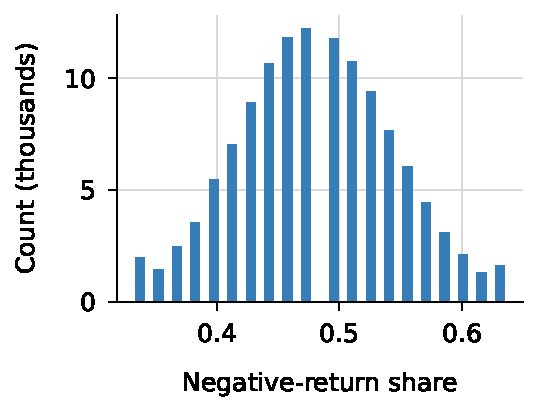
\includegraphics[width=\linewidth]{04_00_market_feature_distribution_09_negative_return_share_63d.pdf}
        \end{subfigure}
        \caption[Training-sample distributions of market predictors]{Training-sample distributions of the nine market predictors. Values are clipped at their 1st and 99th percentiles for display only.}
        \label{fig:market-feature-distributions}
\end{figure}

\noindent
Figure~\ref{fig:market-temporal-stability} tracks the quarterly medians of the market predictors over the training period. Their evolution reinforces the use of chronological validation and fitting-sample preprocessing rather than parameters estimated once from the full panel.

\begin{figure}[H]
        \centering
        \begin{subfigure}[t]{0.31\textwidth}
                \centering
                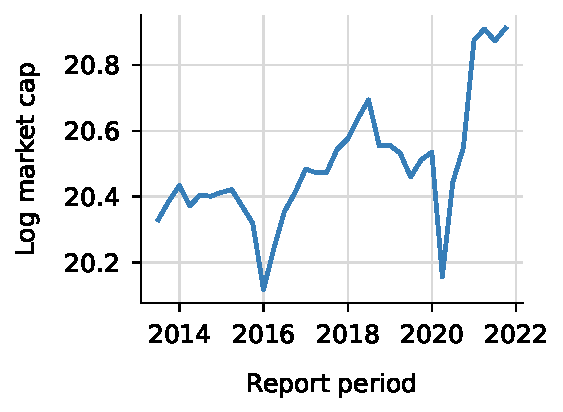
\includegraphics[width=\linewidth]{04_00_market_temporal_stability_01_market_cap_usd.pdf}
        \end{subfigure}
        \hfill
        \begin{subfigure}[t]{0.31\textwidth}
                \centering
                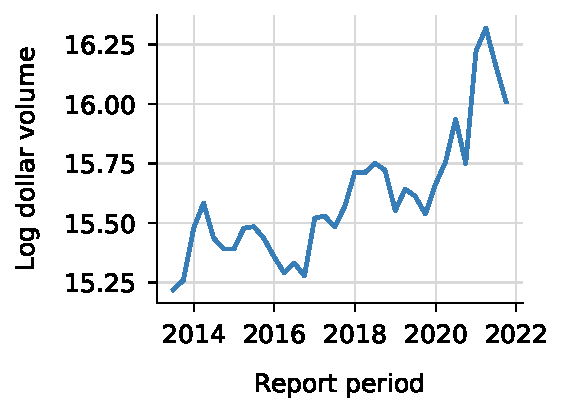
\includegraphics[width=\linewidth]{04_00_market_temporal_stability_02_average_daily_dollar_volume_63d.pdf}
        \end{subfigure}
        \hfill
        \begin{subfigure}[t]{0.31\textwidth}
                \centering
                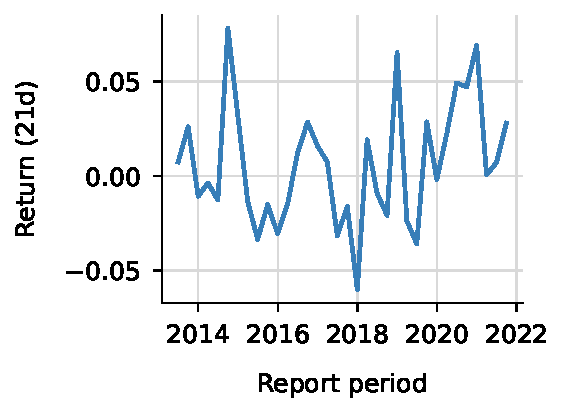
\includegraphics[width=\linewidth]{04_00_market_temporal_stability_03_return_21d.pdf}
        \end{subfigure}
        \par\medskip
        \begin{subfigure}[t]{0.31\textwidth}
                \centering
                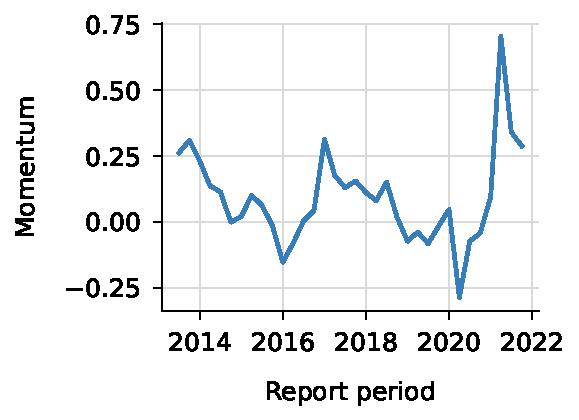
\includegraphics[width=\linewidth]{04_00_market_temporal_stability_04_momentum_252_21d.pdf}
        \end{subfigure}
        \hfill
        \begin{subfigure}[t]{0.31\textwidth}
                \centering
                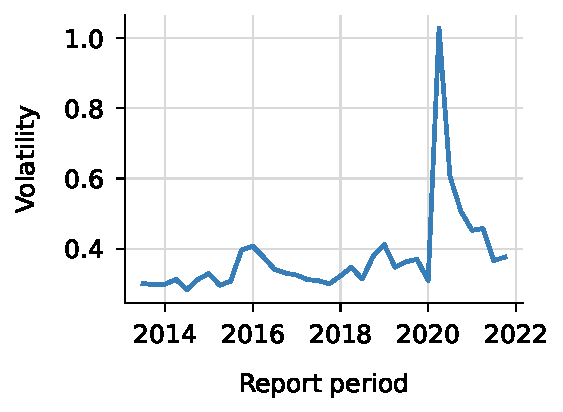
\includegraphics[width=\linewidth]{04_00_market_temporal_stability_05_volatility_63d.pdf}
        \end{subfigure}
        \hfill
        \begin{subfigure}[t]{0.31\textwidth}
                \centering
                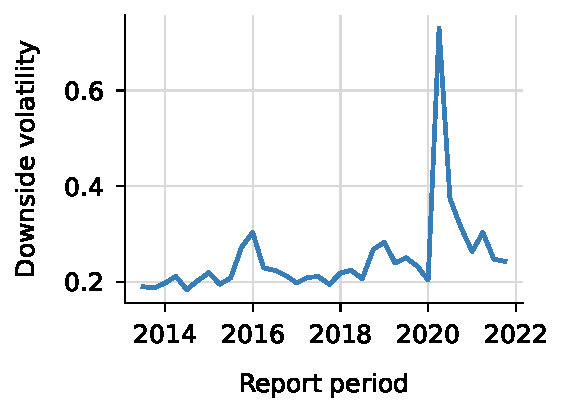
\includegraphics[width=\linewidth]{04_00_market_temporal_stability_06_downside_volatility_63d.pdf}
        \end{subfigure}
        \par\medskip
        \begin{subfigure}[t]{0.31\textwidth}
                \centering
                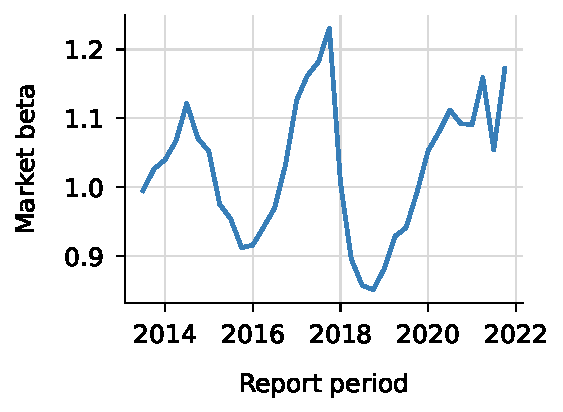
\includegraphics[width=\linewidth]{04_00_market_temporal_stability_07_market_beta_252d.pdf}
        \end{subfigure}
        \hfill
        \begin{subfigure}[t]{0.31\textwidth}
                \centering
                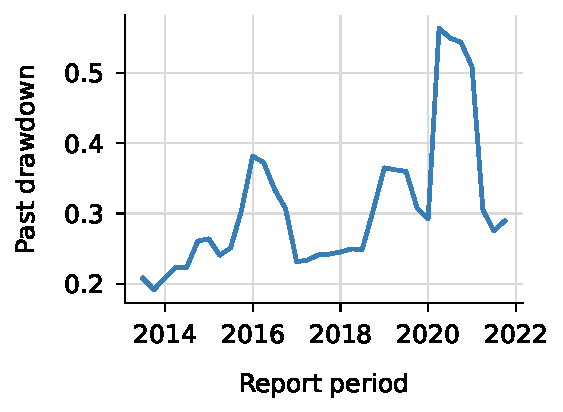
\includegraphics[width=\linewidth]{04_00_market_temporal_stability_08_maximum_drawdown_252d.pdf}
        \end{subfigure}
        \hfill
        \begin{subfigure}[t]{0.31\textwidth}
                \centering
                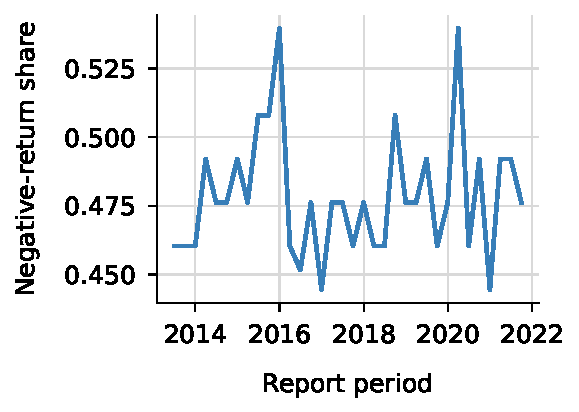
\includegraphics[width=\linewidth]{04_00_market_temporal_stability_09_negative_return_share_63d.pdf}
        \end{subfigure}
        \caption[Temporal stability of market predictors]{Quarterly medians of the market predictors across the training sample.}
        \label{fig:market-temporal-stability}
\end{figure}

\section{Ownership Feature Definitions and Diagnostics}
\label{app:crowding_measures}

Let $v_{m,i,q}$ denote manager $m$'s reported position value in stock $i$ during quarter $q$, $V_{i,q}=\sum_m v_{m,i,q}$ the stock's total reported institutional value, $P_{m,q}=\sum_j v_{m,j,q}$ manager $m$'s total reported portfolio value, $p_{m,i,q}=v_{m,i,q}/P_{m,q}$ the position's portfolio weight, and $M_q$ the number of reporting managers represented in the quarterly network. Table~\ref{tab:ownership-feature-definitions} defines the eleven conventional ownership predictors.

\begingroup
\scriptsize
\setlength{\tabcolsep}{4pt}
\renewcommand{\arraystretch}{1.15}
\begin{longtable}{>{\raggedright\arraybackslash}p{0.23\textwidth}>{\raggedright\arraybackslash}p{0.51\textwidth}>{\raggedright\arraybackslash}p{0.16\textwidth}}
        \caption{Exact definitions of the conventional ownership predictors}
        \label{tab:ownership-feature-definitions}                                                                                                                                              \\
        \toprule
        Feature & Exact construction                                                                                                                                       & Construction rule \\
        \midrule
        \endfirsthead
        \toprule
        Feature & Exact construction                                                                                                                                       & Construction rule \\
        \midrule
        \endhead
        \bottomrule
        \endfoot
        \nolinkurl{institutional_holder_count}
                & Number of distinct reporting managers with a retained position in the stock.
                & Calculated in levels.                                                                                                                                                        \\
        \nolinkurl{total_reported_value_usd}
                & $V_{i,q}=\sum_m v_{m,i,q}$.
                & Calculated in levels.                                                                                                                                                        \\
        \nolinkurl{reported_ownership_hhi}
                & $\sum_m (v_{m,i,q}/V_{i,q})^2$; concentration is measured within the stock's reported institutional ownership, not relative to total shares outstanding.
                & Used in levels.                                                                                                                                                              \\
        \nolinkurl{top_five_reported_ownership_share}
                & Sum of $v_{m,i,q}/V_{i,q}$ across the five managers with the largest reported position values in the stock.
                & Used in levels.                                                                                                                                                              \\
        \nolinkurl{mean_owner_portfolio_weight}
                & Unweighted mean of $p_{m,i,q}$ across the stock's reporting owners.
                & Used in levels.                                                                                                                                                              \\
        \nolinkurl{maximum_owner_portfolio_weight}
                & Maximum value of $p_{m,i,q}$ across the stock's reporting owners.
                & Used in levels.                                                                                                                                                              \\
        \nolinkurl{manager_holder_share}
                & Institutional holder count divided by $M_q$, the total number of reporting managers represented in quarter $q$.
                & Used in levels.                                                                                                                                                              \\
        \nolinkurl{institutional_holder_count_change_percent}
                & $100(H_{i,q}-H_{i,q-1})/H_{i,q-1}$, where $H_{i,q}$ is the institutional holder count.
                & Defined only for consecutive observed quarters.                                                                                                                              \\
        \nolinkurl{total_reported_value_change_percent}
                & $100(V_{i,q}-V_{i,q-1})/V_{i,q-1}$.
                & Defined only for consecutive observed quarters.                                                                                                                              \\
        \nolinkurl{reported_ownership_hhi_change}
                & $\mathrm{HHI}_{i,q}-\mathrm{HHI}_{i,q-1}$, an absolute rather than percentage change.
                & Defined only for consecutive observed quarters.                                                                                                                              \\
        \nolinkurl{top_five_reported_ownership_share_change}
                & Difference between the current and preceding quarter's top-five reported-ownership share.
                & Defined only for consecutive observed quarters.                                                                                                                              \\
\end{longtable}
\endgroup

\noindent
The level features require at least one retained manager position and have no rolling minimum-observation requirement. Change features require observations in consecutive reporting quarters. Missing change measures remain distinguishable at construction and are addressed only within the model preprocessing pipeline.

Figure~\ref{fig:ownership-feature-distributions} summarizes the training-sample distributions of the eleven conventional ownership predictors. Display-only clipping does not alter the values used in the analysis.

\begin{figure}[H]
        \centering
        \begin{subfigure}[t]{0.31\textwidth}
                \centering
                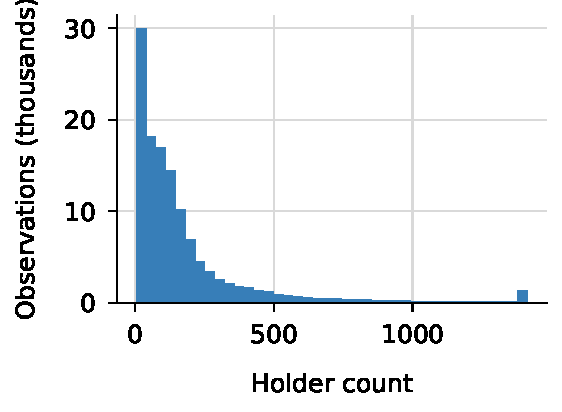
\includegraphics[width=\linewidth]{04_00_ownership_feature_distribution_01_institutional_holder_count.pdf}
        \end{subfigure}
        \hfill
        \begin{subfigure}[t]{0.31\textwidth}
                \centering
                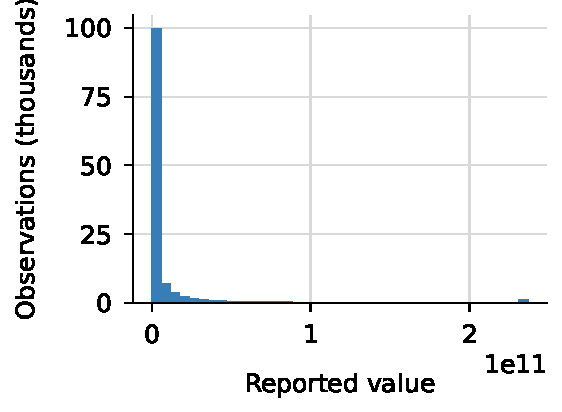
\includegraphics[width=\linewidth]{04_00_ownership_feature_distribution_02_total_reported_value_usd.pdf}
        \end{subfigure}
        \hfill
        \begin{subfigure}[t]{0.31\textwidth}
                \centering
                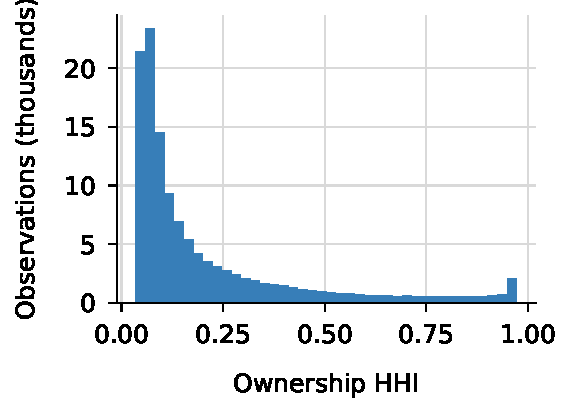
\includegraphics[width=\linewidth]{04_00_ownership_feature_distribution_03_reported_ownership_hhi.pdf}
        \end{subfigure}
        \par\medskip
        \begin{subfigure}[t]{0.31\textwidth}
                \centering
                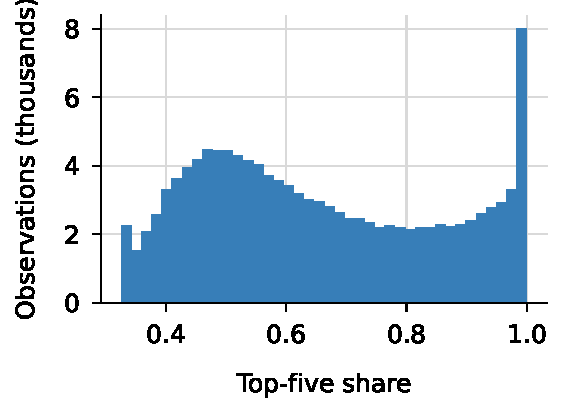
\includegraphics[width=\linewidth]{04_00_ownership_feature_distribution_04_top_five_reported_ownership_share.pdf}
        \end{subfigure}
        \hfill
        \begin{subfigure}[t]{0.31\textwidth}
                \centering
                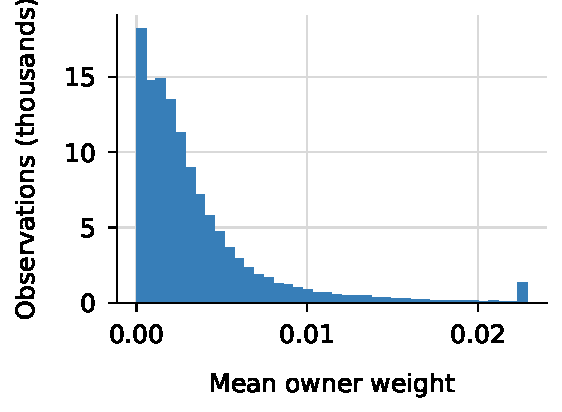
\includegraphics[width=\linewidth]{04_00_ownership_feature_distribution_05_mean_owner_portfolio_weight.pdf}
        \end{subfigure}
        \hfill
        \begin{subfigure}[t]{0.31\textwidth}
                \centering
                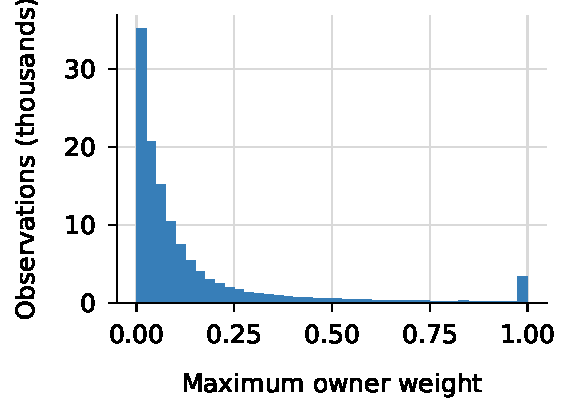
\includegraphics[width=\linewidth]{04_00_ownership_feature_distribution_06_maximum_owner_portfolio_weight.pdf}
        \end{subfigure}
        \par\medskip
        \begin{subfigure}[t]{0.31\textwidth}
                \centering
                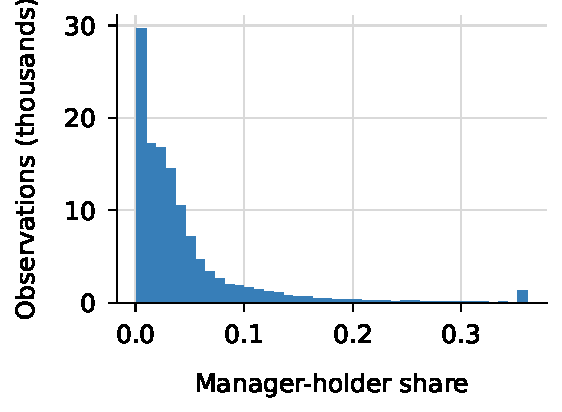
\includegraphics[width=\linewidth]{04_00_ownership_feature_distribution_07_manager_holder_share.pdf}
        \end{subfigure}
        \hfill
        \begin{subfigure}[t]{0.31\textwidth}
                \centering
                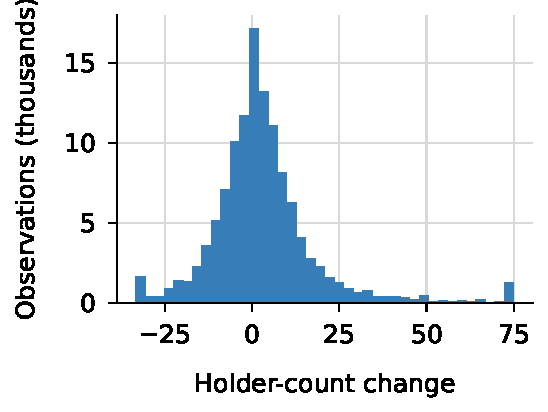
\includegraphics[width=\linewidth]{04_00_ownership_feature_distribution_08_institutional_holder_count_change_percent.pdf}
        \end{subfigure}
        \hfill
        \begin{subfigure}[t]{0.31\textwidth}
                \centering
                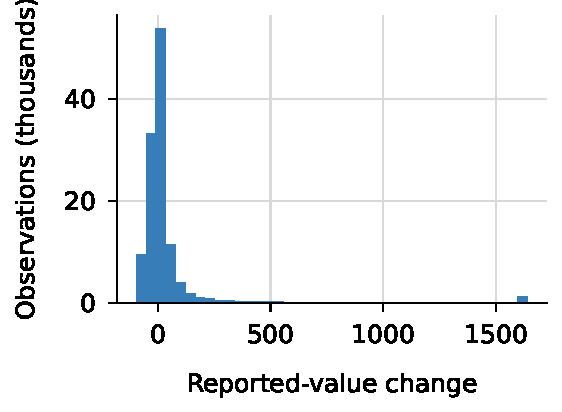
\includegraphics[width=\linewidth]{04_00_ownership_feature_distribution_09_total_reported_value_change_percent.pdf}
        \end{subfigure}
        \par\medskip
        \makebox[\textwidth][c]{%
                \begin{subfigure}[t]{0.31\textwidth}
                        \centering
                        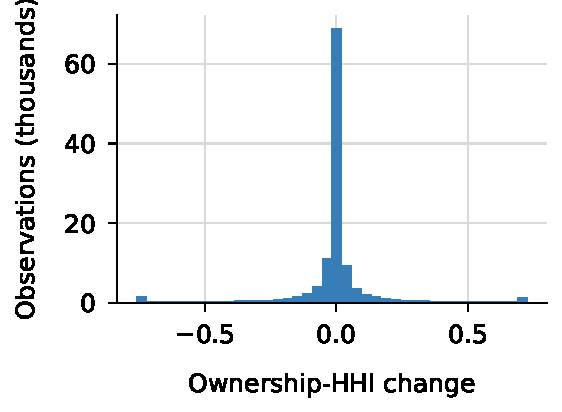
\includegraphics[width=\linewidth]{04_00_ownership_feature_distribution_10_reported_ownership_hhi_change.pdf}
                \end{subfigure}%
                \hspace{0.02\textwidth}%
                \begin{subfigure}[t]{0.31\textwidth}
                        \centering
                        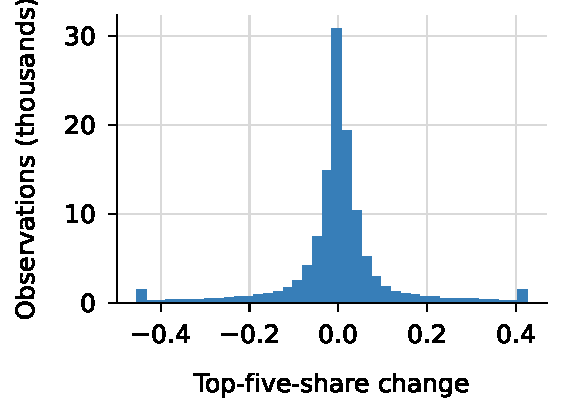
\includegraphics[width=\linewidth]{04_00_ownership_feature_distribution_11_top_five_reported_ownership_share_change.pdf}
                \end{subfigure}%
        }
        \caption[Training-sample distributions of ownership predictors]{Training-sample distributions of the eleven conventional ownership predictors. Values are clipped at their 1st and 99th percentiles for display only.}
        \label{fig:ownership-feature-distributions}
\end{figure}

\noindent
Figure~\ref{fig:ownership-temporal-stability} reports the quarterly medians of the conventional ownership predictors over the training period. The observed changes through time support estimating preprocessing parameters from the fitting sample and assessing predictive performance chronologically.

\begin{figure}[H]
        \centering
        \begin{subfigure}[t]{0.31\textwidth}
                \centering
                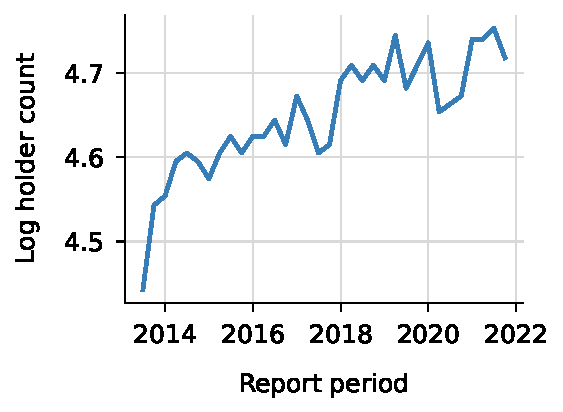
\includegraphics[width=\linewidth]{04_00_ownership_temporal_stability_01_institutional_holder_count.pdf}
        \end{subfigure}
        \hfill
        \begin{subfigure}[t]{0.31\textwidth}
                \centering
                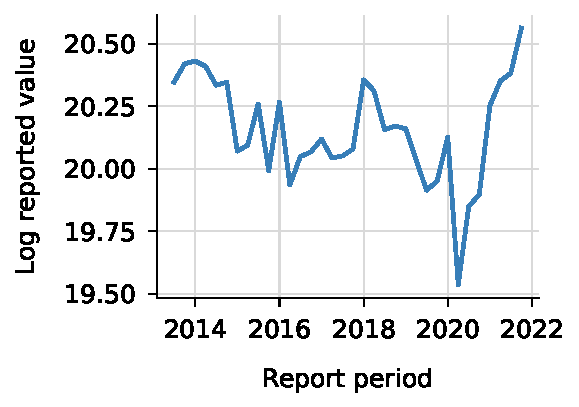
\includegraphics[width=\linewidth]{04_00_ownership_temporal_stability_02_total_reported_value_usd.pdf}
        \end{subfigure}
        \hfill
        \begin{subfigure}[t]{0.31\textwidth}
                \centering
                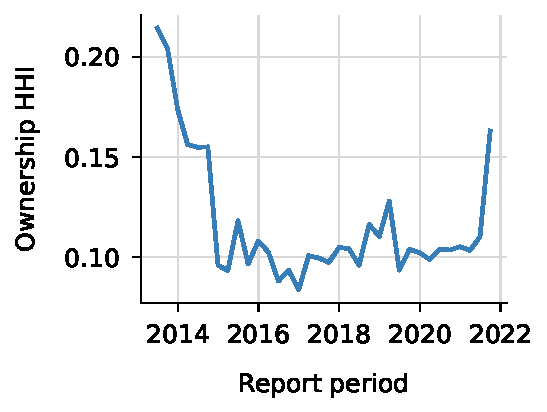
\includegraphics[width=\linewidth]{04_00_ownership_temporal_stability_03_reported_ownership_hhi.pdf}
        \end{subfigure}
        \par\medskip
        \begin{subfigure}[t]{0.31\textwidth}
                \centering
                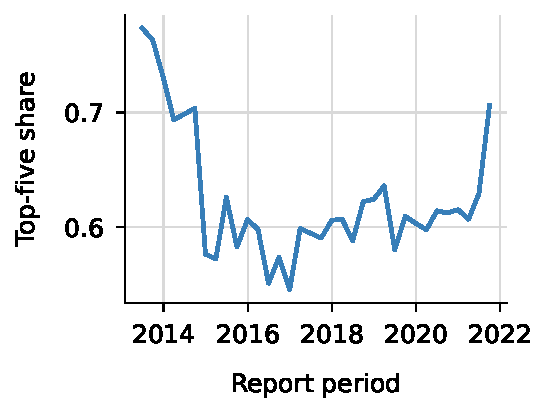
\includegraphics[width=\linewidth]{04_00_ownership_temporal_stability_04_top_five_reported_ownership_share.pdf}
        \end{subfigure}
        \hfill
        \begin{subfigure}[t]{0.31\textwidth}
                \centering
                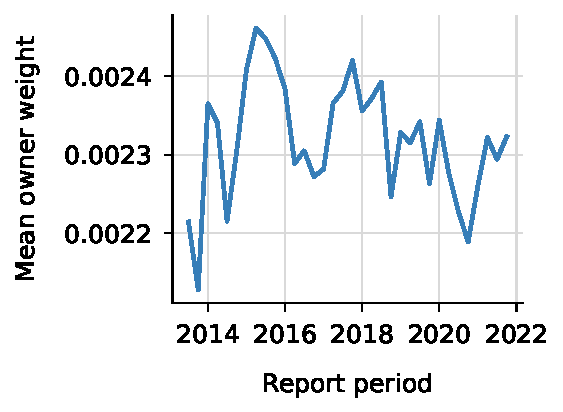
\includegraphics[width=\linewidth]{04_00_ownership_temporal_stability_05_mean_owner_portfolio_weight.pdf}
        \end{subfigure}
        \hfill
        \begin{subfigure}[t]{0.31\textwidth}
                \centering
                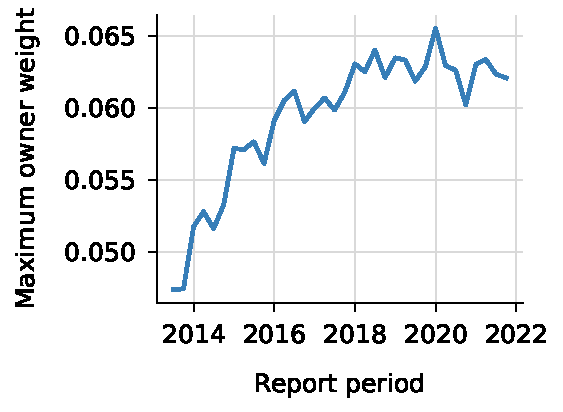
\includegraphics[width=\linewidth]{04_00_ownership_temporal_stability_06_maximum_owner_portfolio_weight.pdf}
        \end{subfigure}
        \par\medskip
        \begin{subfigure}[t]{0.31\textwidth}
                \centering
                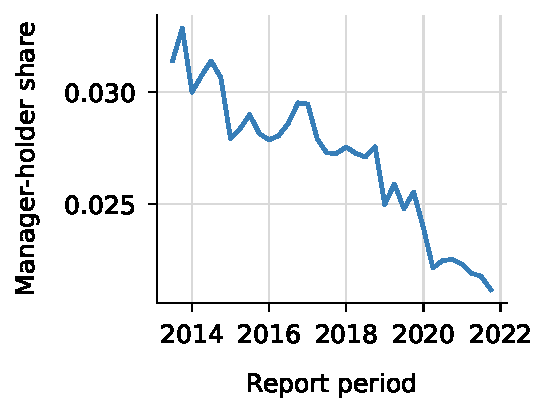
\includegraphics[width=\linewidth]{04_00_ownership_temporal_stability_07_manager_holder_share.pdf}
        \end{subfigure}
        \hfill
        \begin{subfigure}[t]{0.31\textwidth}
                \centering
                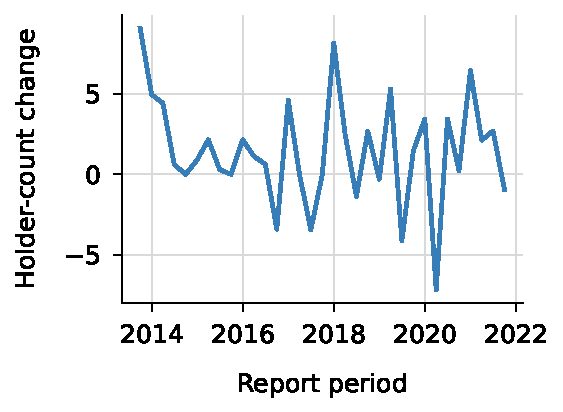
\includegraphics[width=\linewidth]{04_00_ownership_temporal_stability_08_institutional_holder_count_change_percent.pdf}
        \end{subfigure}
        \hfill
        \begin{subfigure}[t]{0.31\textwidth}
                \centering
                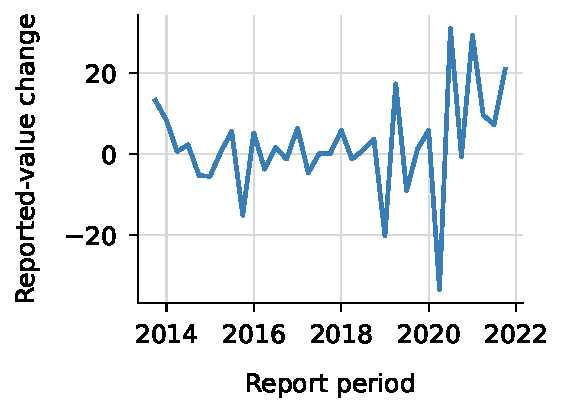
\includegraphics[width=\linewidth]{04_00_ownership_temporal_stability_09_total_reported_value_change_percent.pdf}
        \end{subfigure}
        \par\medskip
        \makebox[\textwidth][c]{%
                \begin{subfigure}[t]{0.31\textwidth}
                        \centering
                        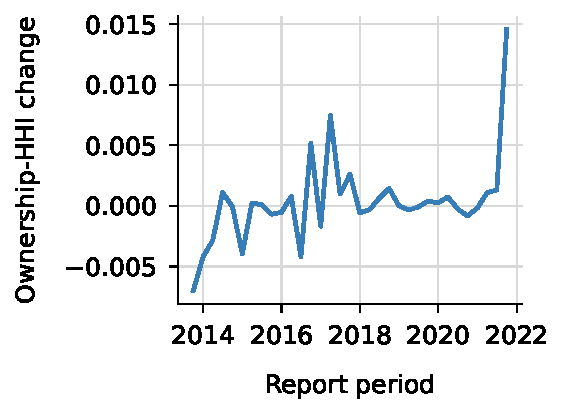
\includegraphics[width=\linewidth]{04_00_ownership_temporal_stability_10_reported_ownership_hhi_change.pdf}
                \end{subfigure}%
                \hspace{0.02\textwidth}%
                \begin{subfigure}[t]{0.31\textwidth}
                        \centering
                        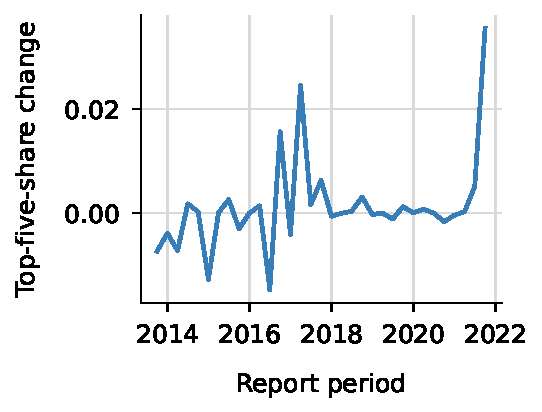
\includegraphics[width=\linewidth]{04_00_ownership_temporal_stability_11_top_five_reported_ownership_share_change.pdf}
                \end{subfigure}%
        }
        \caption[Temporal stability of ownership predictors]{Quarterly medians of the conventional ownership predictors across the training sample.}
        \label{fig:ownership-temporal-stability}
\end{figure}

\section{Ownership Network and Features}
\label{app:ownership_network}

\subsection{Bipartite Manager--Stock Network}
\label{app:bipartite_graph}

Figure~\ref{fig:network-growth} summarizes the growth of the quarterly ownership network in its two node sets and reported ownership edges.

\begin{figure}[H]
        \centering
        \begin{subfigure}[t]{0.48\textwidth}
                \centering
                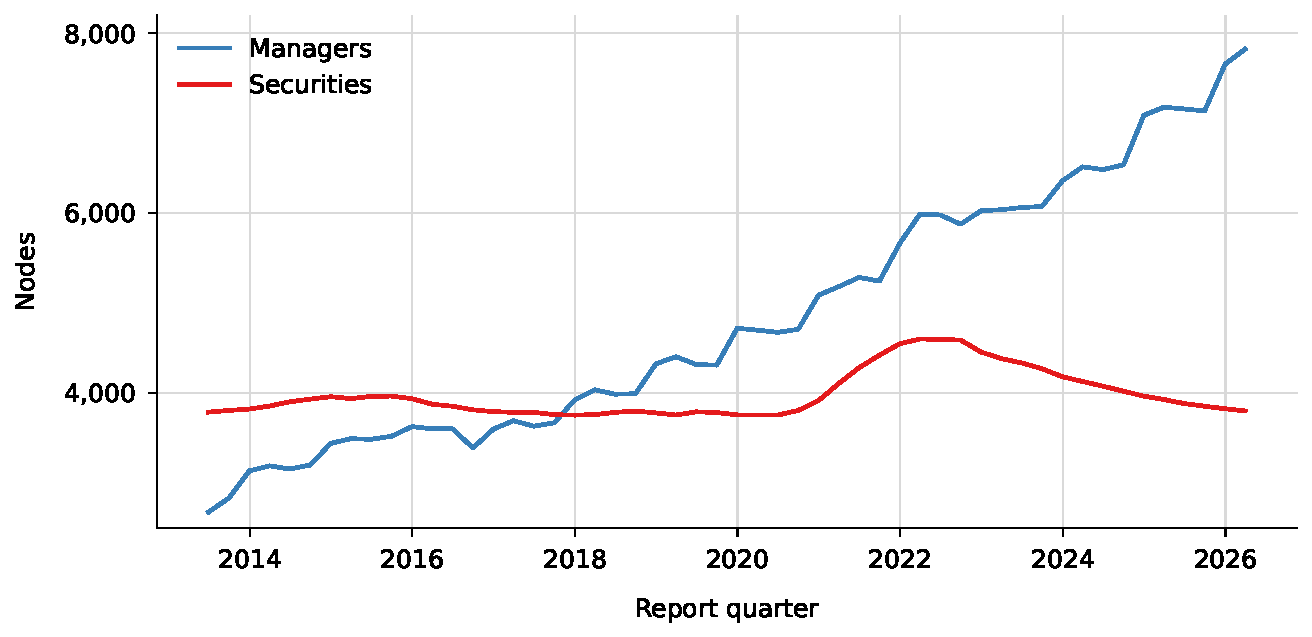
\includegraphics[width=\linewidth]{02_01_network_nodes_matplotlib.pdf}
                \caption{Manager and security nodes.}
        \end{subfigure}
        \hfill
        \begin{subfigure}[t]{0.48\textwidth}
                \centering
                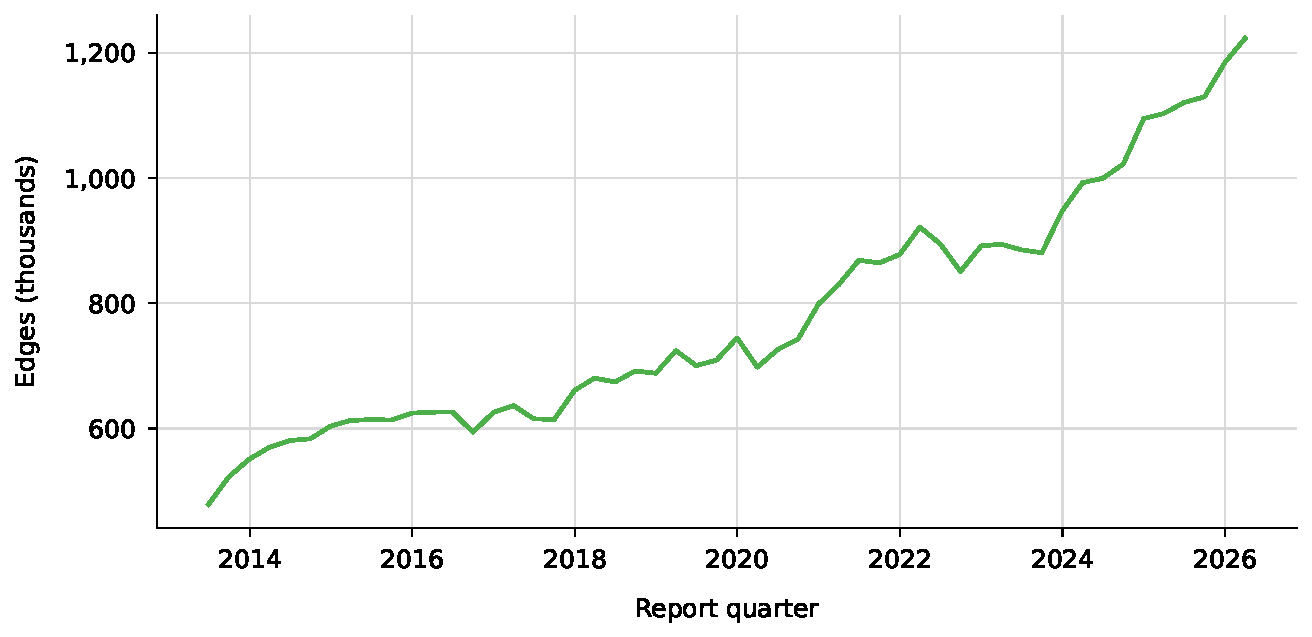
\includegraphics[width=\linewidth]{02_01_network_edges_matplotlib.pdf}
                \caption{Ownership edges.}
        \end{subfigure}
        \caption{Evolution of the quarterly institutional ownership network.}
        \label{fig:network-growth}
\end{figure}

\noindent
The quarterly bipartite graphs are large but sparse. Their density ranges from 3.16\% to 4.86\% of all possible manager--security pairs, while every quarterly graph forms a single connected component. Thus, any two securities are connected through some chain of shared owners even though most possible ownership edges do not exist. A full quarterly graph is not directly legible because a typical snapshot contains several thousand managers, a comparable number of securities, and hundreds of thousands of ownership edges; the edge count exceeds one million in later quarters.

Figure~\ref{fig:network-degree-distributions} reports the pooled distributions of securities held per manager and institutional holders per stock across the quarterly ownership networks. Both are strongly right-skewed: most nodes have comparatively low degree, while a smaller group of managers holds many securities and a smaller group of stocks is held by many institutions.

\begin{figure}[H]
        \centering
        \begin{subfigure}[t]{0.48\textwidth}
                \centering
                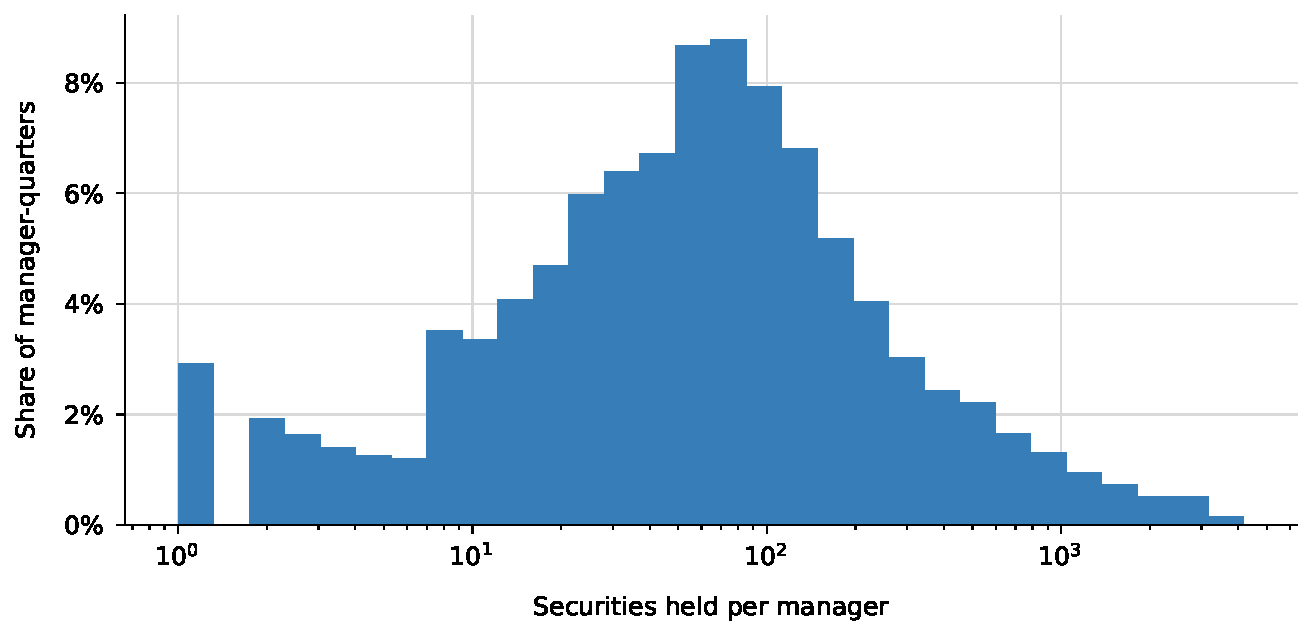
\includegraphics[width=\linewidth]{08_01_manager_degree_distribution.pdf}
                \caption{Securities held per manager.}
                \label{fig:manager-degree-distribution}
        \end{subfigure}
        \hfill
        \begin{subfigure}[t]{0.48\textwidth}
                \centering
                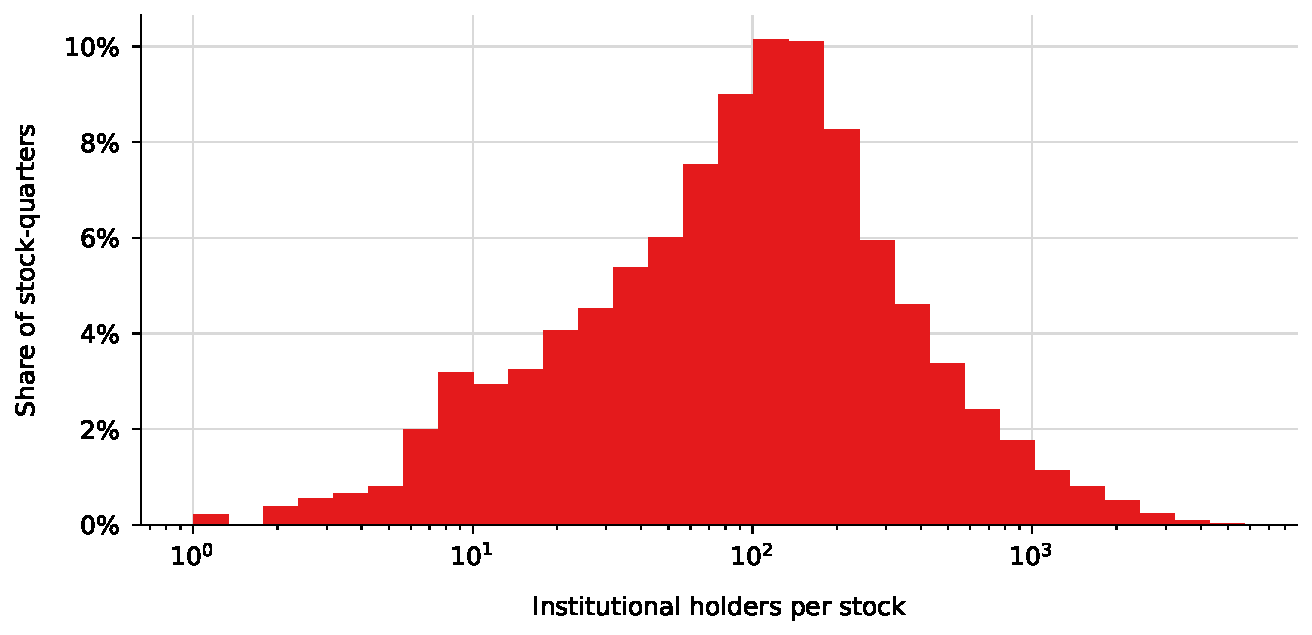
\includegraphics[width=\linewidth]{08_01_stock_degree_distribution.pdf}
                \caption{Institutional holders per stock.}
                \label{fig:stock-degree-distribution}
        \end{subfigure}
        \caption[Node-degree distributions in the ownership network]{Pooled distributions of manager and stock node degrees across the quarterly ownership networks. Counts are shown in their original units on logarithmic horizontal axes.}
        \label{fig:network-degree-distributions}
\end{figure}

\subsection{Manager Similarity and Communities}
\label{app:manager_similarity}

Managers are compared using their quarterly vectors of portfolio weights. For managers \(m\) and \(n\), portfolio similarity is measured by cosine similarity,

\begin{equation}
        \operatorname{sim}_{m,n,q}
        =
        \frac{\mathbf{p}_{m,q}^{\prime}\mathbf{p}_{n,q}}
        {\lVert\mathbf{p}_{m,q}\rVert\lVert\mathbf{p}_{n,q}\rVert},
        \label{eq:manager_cosine_similarity}
\end{equation}

\noindent
where \(\mathbf{p}_{m,q}\) contains manager \(m\)'s portfolio weights in quarter \(q\). Each manager is connected to its 25 nearest positive-similarity neighbours. The resulting relations are converted into an undirected weighted graph, and Louvain community detection is applied separately in each quarter \parencite{blondel2008fast}. Managers in the same community therefore hold relatively similar portfolios within that quarter; community labels are not treated as persistent identities through time.

Figure~\ref{fig:manager-community-evolution} summarizes the resulting community structure. The number of detected communities generally increases, while the share of managers in the largest community declines. This pattern indicates that the expanding manager population becomes divided among a broader set of contemporaneous portfolio-similarity groups.

\begin{figure}[H]
        \centering
        \begin{subfigure}[t]{0.48\textwidth}
                \centering
                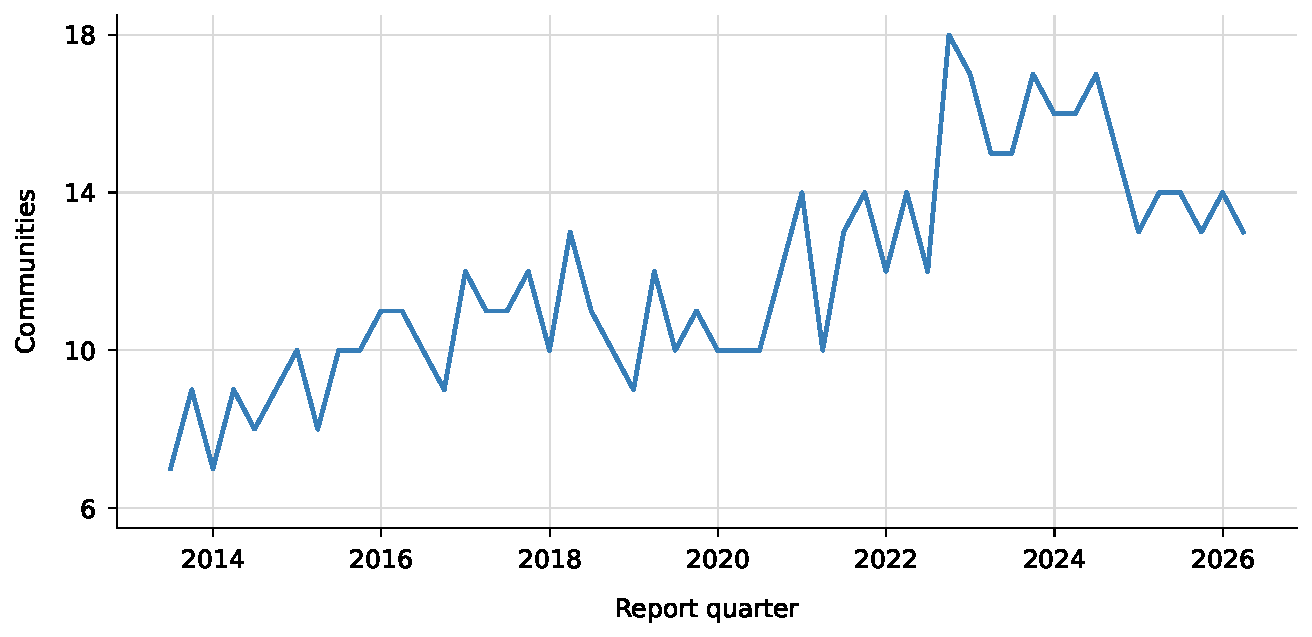
\includegraphics[width=\linewidth]{02_02_community_count_matplotlib.pdf}
                \caption{Number of communities.}
        \end{subfigure}
        \hfill
        \begin{subfigure}[t]{0.48\textwidth}
                \centering
                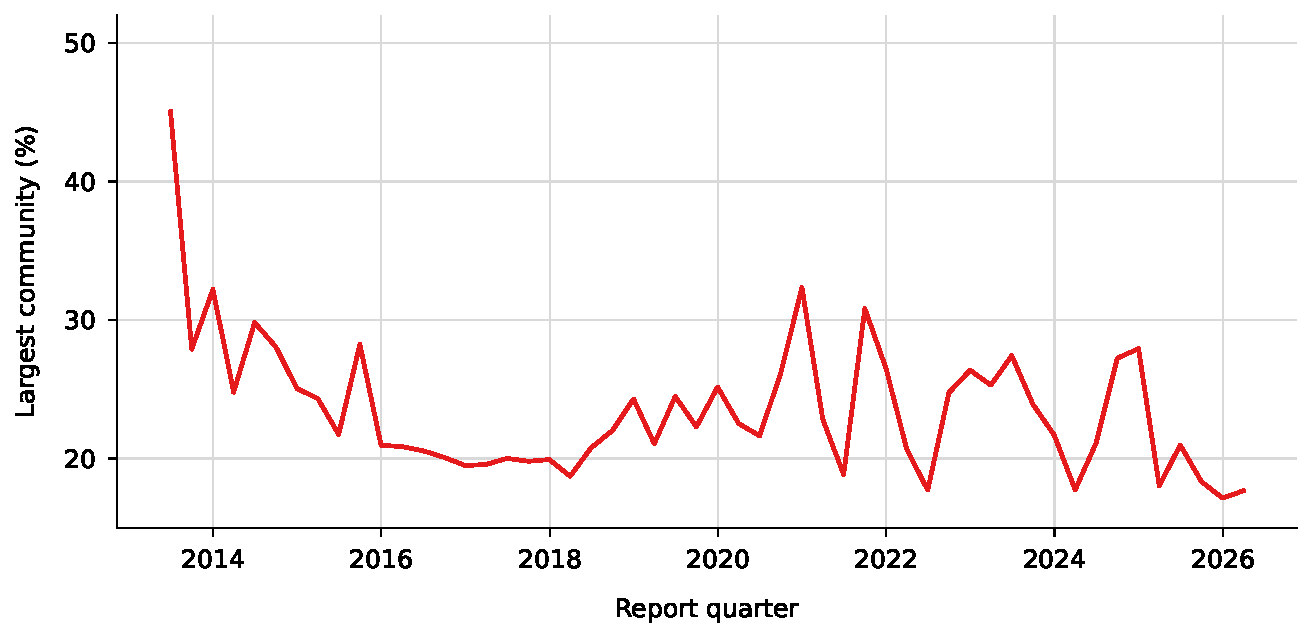
\includegraphics[width=\linewidth]{02_02_largest_community_share_matplotlib.pdf}
                \caption{Largest-community share.}
        \end{subfigure}
        \caption[Quarterly manager-community structure]{Number of manager communities and share of managers in the largest community by reporting quarter.}
        \label{fig:manager-community-evolution}
\end{figure}

\noindent
Across the pooled quarterly sample, the 25-nearest-neighbor manager-similarity graphs contain 5,627,437 edges. Applying Louvain community detection separately in each quarter produces between 7 and 18 communities, with a median of 11.5. Figure~\ref{fig:community-meta-graph} illustrates this structure for the final test quarter. Each detected community is collapsed into a single node, whose size represents its manager count, and the strongest inter-community similarity links are retained for display.

\begin{figure}[H]
        \centering
        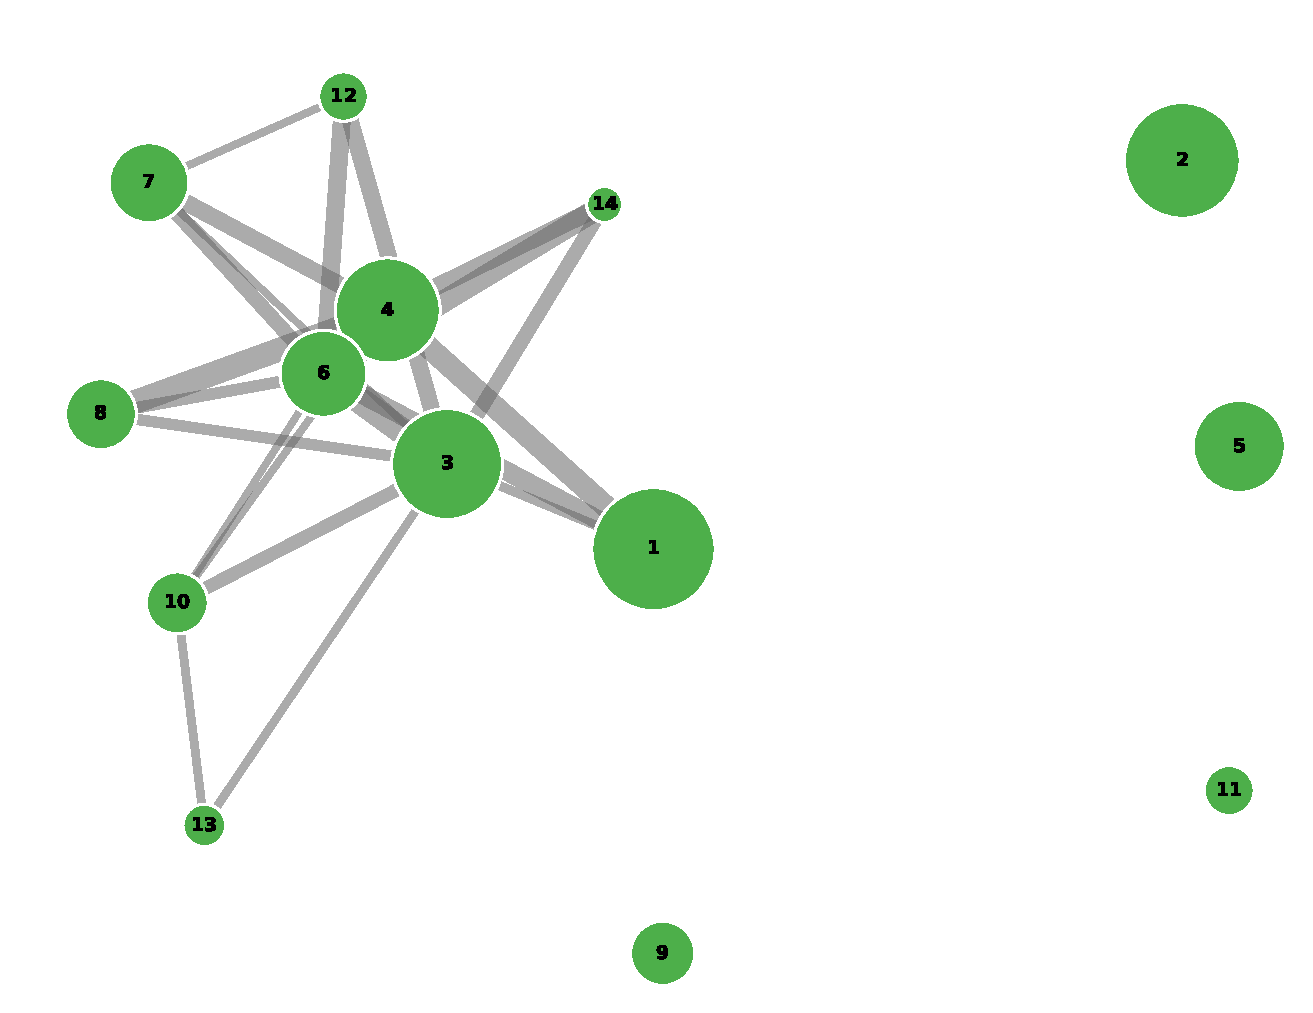
\includegraphics[width=0.75\textwidth]{08_01_community_meta_graph.pdf}
        \caption[Manager-community meta-graph]{Manager communities in the illustrative quarter, collapsed to one node per community, with node size representing manager count and the strongest inter-community similarity links displayed.}
        \label{fig:community-meta-graph}
\end{figure}

\subsection{Network Feature Definitions and Diagnostics}
\label{app:network_features}

For each quarter, manager portfolios are represented by vectors of reported portfolio weights. Cosine similarity is calculated between these vectors, and each manager is linked to its 25 nearest positive-similarity neighbours. The directed neighbour relations are converted into an undirected union graph, retaining the larger similarity when a relation is observed in both directions. Louvain communities are estimated on this weighted graph with resolution 1 and random seed 13. Let $a_{m,i,q}=v_{m,i,q}/V_{i,q}$ denote manager $m$'s share of stock $i$'s reported institutional value, $d_{m,q}$ its degree in the manager-similarity graph, $M_q$ the number of managers, and $\bar{s}_{m,q}$ its mean similarity to graph neighbours. Table~\ref{tab:network-feature-definitions} defines the eight resulting stock-level features.

\begingroup
\scriptsize
\setlength{\tabcolsep}{4pt}
\renewcommand{\arraystretch}{1.15}
\begin{longtable}{>{\raggedright\arraybackslash}p{0.24\textwidth}>{\raggedright\arraybackslash}p{0.50\textwidth}>{\raggedright\arraybackslash}p{0.16\textwidth}}
        \caption{Exact definitions of the ownership-network predictors}
        \label{tab:network-feature-definitions}                                                                                                                                                                                             \\
        \toprule
        Feature & Exact construction                                                                                                                                                                                    & Construction rule \\
        \midrule
        \endfirsthead
        \toprule
        Feature & Exact construction                                                                                                                                                                                    & Construction rule \\
        \midrule
        \endhead
        \bottomrule
        \endfoot
        \nolinkurl{owner_similarity_score}
                & Mean cosine similarity across all unordered pairs of the stock's owners. Owner pairs not connected in the 25-nearest-neighbour graph contribute zero; stocks with fewer than two owners receive zero.
                & Calculated in levels.                                                                                                                                                                                                     \\
        \nolinkurl{value_weighted_owner_degree_centrality}
                & $\sum_m a_{m,i,q}\,d_{m,q}/(M_q-1)$.
                & Weighted by reported position value.                                                                                                                                                                                      \\
        \nolinkurl{value_weighted_owner_neighbor_similarity}
                & $\sum_m a_{m,i,q}\,\bar{s}_{m,q}$.
                & Weighted by reported position value.                                                                                                                                                                                      \\
        \nolinkurl{owner_community_count}
                & Number of distinct contemporaneous Louvain communities represented among the stock's owners.
                & Calculated in levels.                                                                                                                                                                                                     \\
        \nolinkurl{owner_community_hhi}
                & $\sum_c A_{c,i,q}^2$, where $A_{c,i,q}=\sum_{m\in c}a_{m,i,q}$ is community $c$'s share of the stock's reported institutional value.
                & Calculated in levels.                                                                                                                                                                                                     \\
        \nolinkurl{largest_owner_community_share}
                & $\max_c A_{c,i,q}$.
                & Calculated in levels.                                                                                                                                                                                                     \\
        \nolinkurl{owner_similarity_score_change}
                & Difference between the current and preceding quarter's owner-similarity score.
                & Defined only for consecutive observed quarters.                                                                                                                                                                           \\
        \nolinkurl{owner_community_hhi_change}
                & Difference between the current and preceding quarter's owner-community HHI.
                & Defined only for consecutive observed quarters.                                                                                                                                                                           \\
\end{longtable}
\endgroup

\noindent
The level features require at least one retained owner, except that owner similarity is set to zero for stocks with fewer than two owners. Change features require observations in consecutive reporting quarters.

Raw network-feature levels can shift mechanically with the size and composition of the graph. Figure~\ref{fig:network-temporal-stability} tracks the quarterly median of each raw feature alongside the number of reporting managers. Manager count correlates $-0.922$ with median owner similarity, $-0.855$ with degree centrality, $0.803$ with community count, and $0.865$ with neighbor similarity. Because the manager population grows substantially over the sample, these relationships indicate that raw feature levels partly drift for mechanical rather than economic reasons and motivate the within-quarter percentile-rank transformation used in the predictive analysis.

\begin{figure}[H]
        \centering
        \begin{subfigure}[t]{0.48\textwidth}
                \centering
                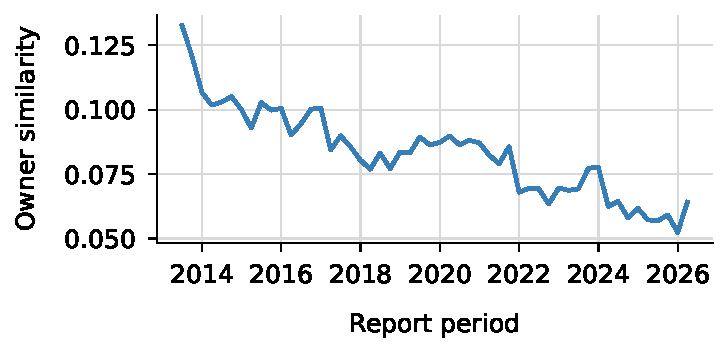
\includegraphics[width=\linewidth]{02_04_temporal_stability_01_owner_similarity_score.pdf}
        \end{subfigure}
        \hfill
        \begin{subfigure}[t]{0.48\textwidth}
                \centering
                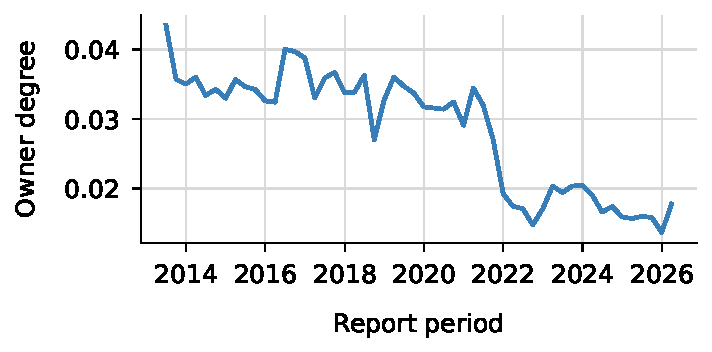
\includegraphics[width=\linewidth]{02_04_temporal_stability_02_value_weighted_owner_degree_centrality.pdf}
        \end{subfigure}
        \par\medskip
        \begin{subfigure}[t]{0.48\textwidth}
                \centering
                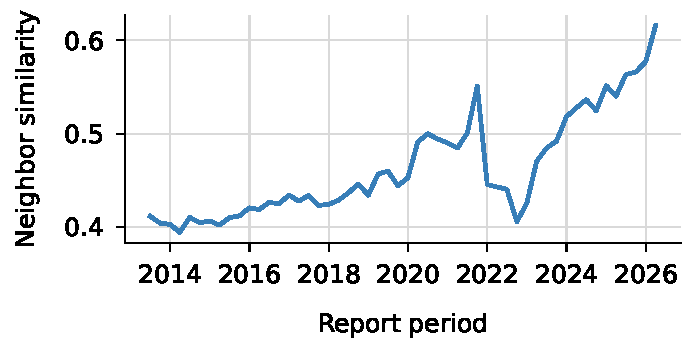
\includegraphics[width=\linewidth]{02_04_temporal_stability_03_value_weighted_owner_neighbor_similarity.pdf}
        \end{subfigure}
        \hfill
        \begin{subfigure}[t]{0.48\textwidth}
                \centering
                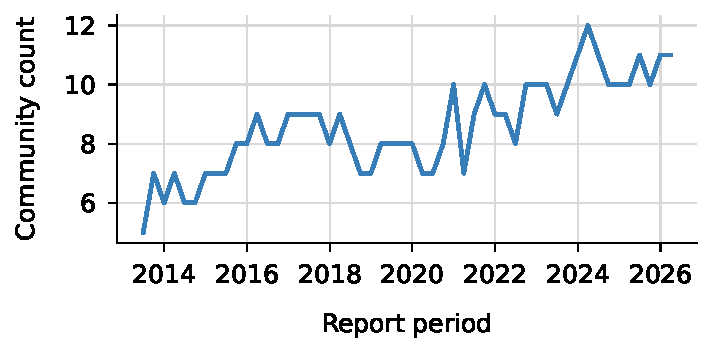
\includegraphics[width=\linewidth]{02_04_temporal_stability_04_owner_community_count.pdf}
        \end{subfigure}
        \par\medskip
        \begin{subfigure}[t]{0.48\textwidth}
                \centering
                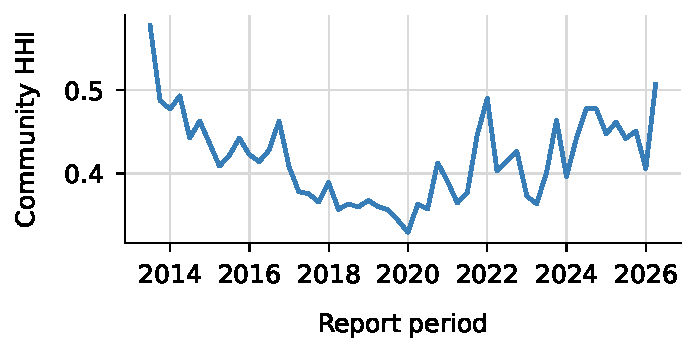
\includegraphics[width=\linewidth]{02_04_temporal_stability_05_owner_community_hhi.pdf}
        \end{subfigure}
        \hfill
        \begin{subfigure}[t]{0.48\textwidth}
                \centering
                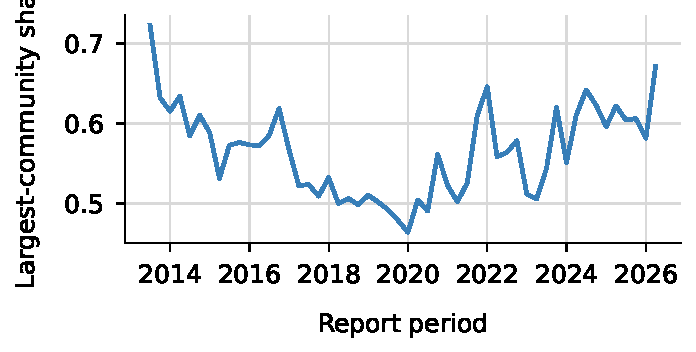
\includegraphics[width=\linewidth]{02_04_temporal_stability_06_largest_owner_community_share.pdf}
        \end{subfigure}
        \par\medskip
        \begin{subfigure}[t]{0.48\textwidth}
                \centering
                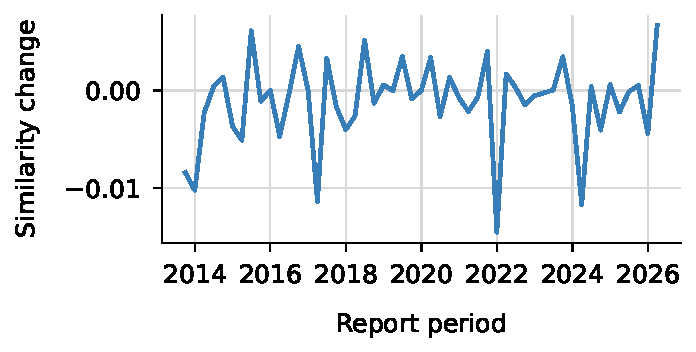
\includegraphics[width=\linewidth]{02_04_temporal_stability_07_owner_similarity_score_change.pdf}
        \end{subfigure}
        \hfill
        \begin{subfigure}[t]{0.48\textwidth}
                \centering
                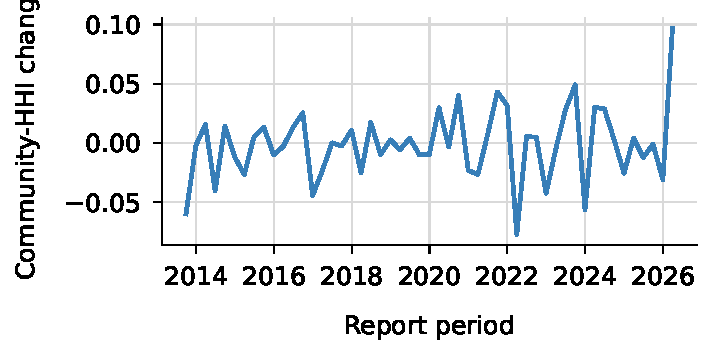
\includegraphics[width=\linewidth]{02_04_temporal_stability_08_owner_community_hhi_change.pdf}
        \end{subfigure}
        \caption[Temporal stability of raw network features]{Quarterly median of each raw network feature across the full sample period, before the within-quarter percentile-rank transformation used in modeling.}
        \label{fig:network-temporal-stability}
\end{figure}

\noindent
Figure~\ref{fig:app-network-distributions} reports the underlying training-sample distributions of the eight network features introduced in Section~\ref{sec:network_features}. Correlations involving these features are evaluated jointly with the market and ownership features in Section~\ref{sec:feature_engineering}.

\begin{figure}[H]
        \centering
        \begin{subfigure}[t]{0.48\textwidth}
                \centering
                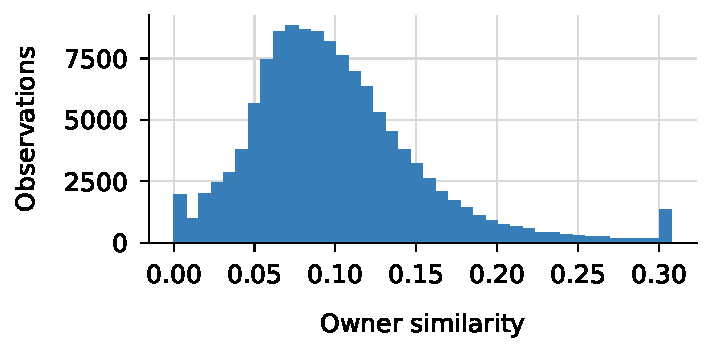
\includegraphics[width=\linewidth]{02_04_feature_distribution_01_owner_similarity_score.pdf}
        \end{subfigure}
        \hfill
        \begin{subfigure}[t]{0.48\textwidth}
                \centering
                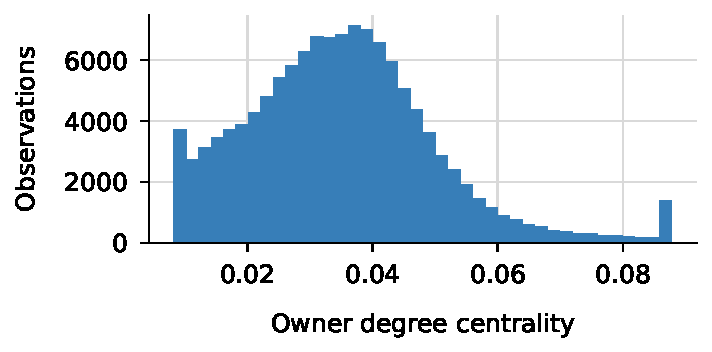
\includegraphics[width=\linewidth]{02_04_feature_distribution_02_value_weighted_owner_degree_centrality.pdf}
        \end{subfigure}
        \par\medskip
        \begin{subfigure}[t]{0.48\textwidth}
                \centering
                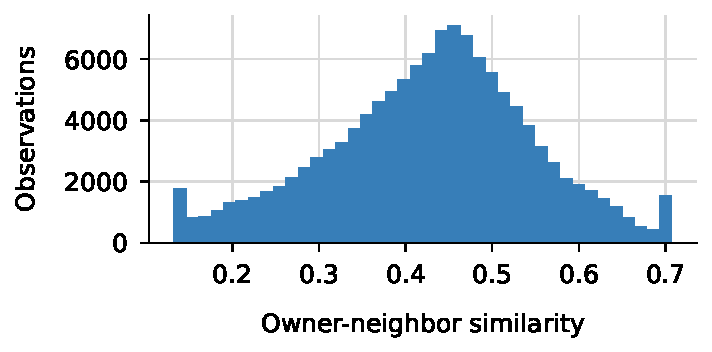
\includegraphics[width=\linewidth]{02_04_feature_distribution_03_value_weighted_owner_neighbor_similarity.pdf}
        \end{subfigure}
        \hfill
        \begin{subfigure}[t]{0.48\textwidth}
                \centering
                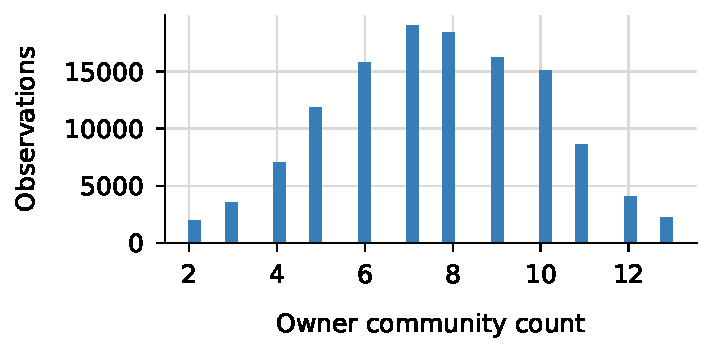
\includegraphics[width=\linewidth]{02_04_feature_distribution_04_owner_community_count.pdf}
        \end{subfigure}
        \par\medskip
        \begin{subfigure}[t]{0.48\textwidth}
                \centering
                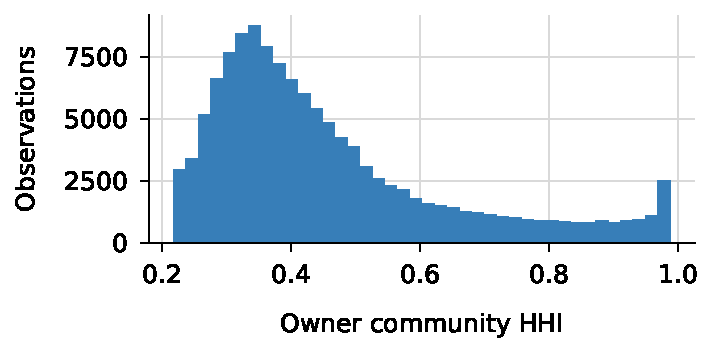
\includegraphics[width=\linewidth]{02_04_feature_distribution_05_owner_community_hhi.pdf}
        \end{subfigure}
        \hfill
        \begin{subfigure}[t]{0.48\textwidth}
                \centering
                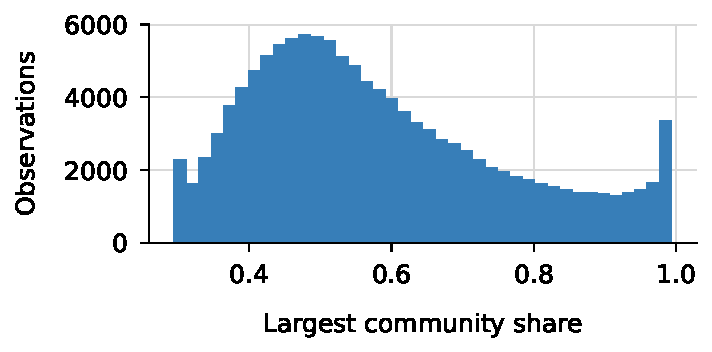
\includegraphics[width=\linewidth]{02_04_feature_distribution_06_largest_owner_community_share.pdf}
        \end{subfigure}
        \par\medskip
        \begin{subfigure}[t]{0.48\textwidth}
                \centering
                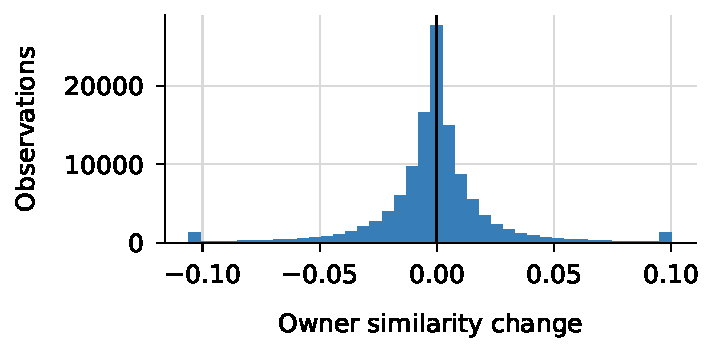
\includegraphics[width=\linewidth]{02_04_feature_distribution_07_owner_similarity_score_change.pdf}
        \end{subfigure}
        \hfill
        \begin{subfigure}[t]{0.48\textwidth}
                \centering
                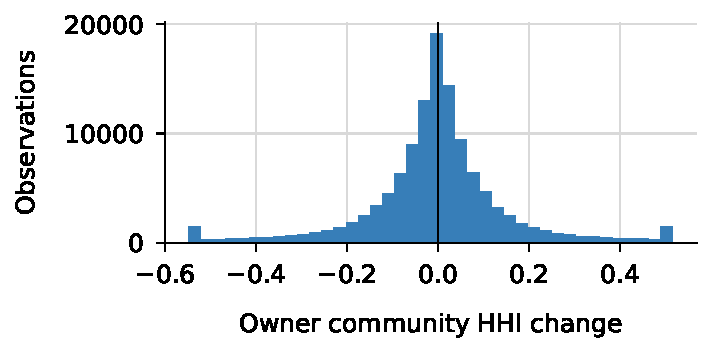
\includegraphics[width=\linewidth]{02_04_feature_distribution_08_owner_community_hhi_change.pdf}
        \end{subfigure}
        \caption[Training-sample network-feature distributions]{Distribution of each of the eight raw network features in the training sample, capped at the 1st and 99th percentiles for display only.}
        \label{fig:app-network-distributions}
\end{figure}

\section{Feature Processing and Selection}
\label{app:feature_processing}

\subsection{Feature Missingness}

Table~\ref{tab:feature-missingness} reports the share of missing observations for every candidate predictor before imputation and redundancy-based feature selection. All market features and all ownership and network level features are complete in the three modeling samples. Missingness is confined to the four ownership-change measures and two network-change measures, which require the stock to be observed in consecutive reporting quarters. Their missing share is higher in the training sample because the beginning of the panel contains no preceding-quarter history, while only a small share of later validation and test observations lacks a consecutive-quarter predecessor.

\begingroup
\footnotesize
\setlength{\tabcolsep}{4pt}
\renewcommand{\arraystretch}{1.08}
\begin{longtable}{p{0.14\textwidth}p{0.40\textwidth}rrr}
    \caption{Missingness across candidate predictors and modeling samples}
    \label{tab:feature-missingness} \\
    \toprule
    Feature group & Feature & \multicolumn{3}{c}{Missing share} \\
    \cmidrule(lr){3-5}
                  &         & Training & Validation & Test \\
    \midrule
    \endfirsthead
    \multicolumn{5}{l}{\footnotesize\itshape Table~\thetable\ continued} \\
    \toprule
    Feature group & Feature & \multicolumn{3}{c}{Missing share} \\
    \cmidrule(lr){3-5}
                  &         & Training & Validation & Test \\
    \midrule
    \endhead
    \midrule
    \multicolumn{5}{r}{\footnotesize\itshape Continued on next page} \\
    \endfoot
    \bottomrule
    \endlastfoot
        Market & Market capitalization & 0.00\% & 0.00\% & 0.00\% \\
        Market & Average daily dollar volume & 0.00\% & 0.00\% & 0.00\% \\
        Market & 21-day return & 0.00\% & 0.00\% & 0.00\% \\
        Market & Skip-month momentum & 0.00\% & 0.00\% & 0.00\% \\
        Market & Volatility & 0.00\% & 0.00\% & 0.00\% \\
        Market & Downside volatility & 0.00\% & 0.00\% & 0.00\% \\
        Market & Market beta & 0.00\% & 0.00\% & 0.00\% \\
        Market & Past maximum drawdown & 0.00\% & 0.00\% & 0.00\% \\
        Market & Negative-return share & 0.00\% & 0.00\% & 0.00\% \\
        Ownership & Institutional holder count & 0.00\% & 0.00\% & 0.00\% \\
        Ownership & Total reported institutional value & 0.00\% & 0.00\% & 0.00\% \\
        Ownership & Ownership HHI & 0.00\% & 0.00\% & 0.00\% \\
        Ownership & Top-five ownership share & 0.00\% & 0.00\% & 0.00\% \\
        Ownership & Mean owner portfolio weight & 0.00\% & 0.00\% & 0.00\% \\
        Ownership & Maximum owner portfolio weight & 0.00\% & 0.00\% & 0.00\% \\
        Ownership & Manager-holder share & 0.00\% & 0.00\% & 0.00\% \\
        Ownership & Change in institutional holder count & 3.02\% & 0.16\% & 0.15\% \\
        Ownership & Change in total reported institutional value & 3.02\% & 0.16\% & 0.15\% \\
        Ownership & Change in ownership HHI & 3.02\% & 0.16\% & 0.15\% \\
        Ownership & Change in top-five ownership share & 3.02\% & 0.16\% & 0.15\% \\
        Network & Owner similarity & 0.00\% & 0.00\% & 0.00\% \\
        Network & Owner degree centrality & 0.00\% & 0.00\% & 0.00\% \\
        Network & Owner-neighbour similarity & 0.00\% & 0.00\% & 0.00\% \\
        Network & Owner community count & 0.00\% & 0.00\% & 0.00\% \\
        Network & Owner-community HHI & 0.00\% & 0.00\% & 0.00\% \\
        Network & Largest owner-community share & 0.00\% & 0.00\% & 0.00\% \\
        Network & Change in owner similarity & 3.02\% & 0.16\% & 0.15\% \\
        Network & Change in owner-community HHI & 3.02\% & 0.16\% & 0.15\% \\
\end{longtable}
\endgroup


\noindent
Market capitalization, average daily dollar volume, institutional holder count, and total reported institutional value are examined under $\log(1+x)$ transformations because their raw distributions are strongly right-skewed. Figure~\ref{fig:log-transformations} shows the two market scale variables, while Figure~\ref{fig:ownership-log-transformations} presents the corresponding ownership variables. After redundancy-based selection, only market capitalization remains in the fitted tabular and stock-node feature sets. Raw distributions are capped at their 99th percentiles for display only.

\begin{figure}[H]
        \centering
        \begin{subfigure}[t]{0.48\textwidth}
                \centering
                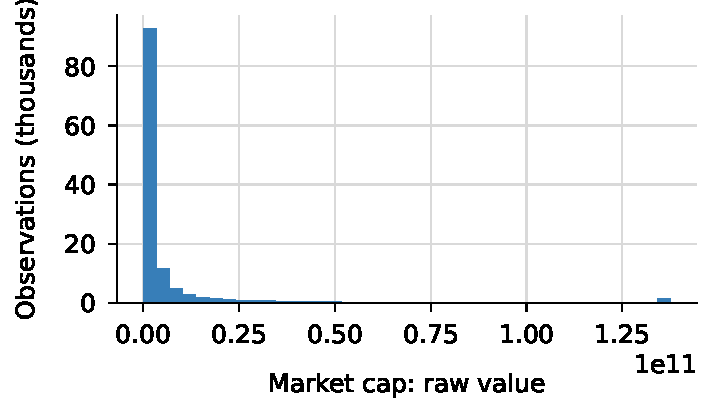
\includegraphics[width=\linewidth]{04_00_market_log_transformation_01_market_cap_usd_raw.pdf}
        \end{subfigure}
        \hfill
        \begin{subfigure}[t]{0.48\textwidth}
                \centering
                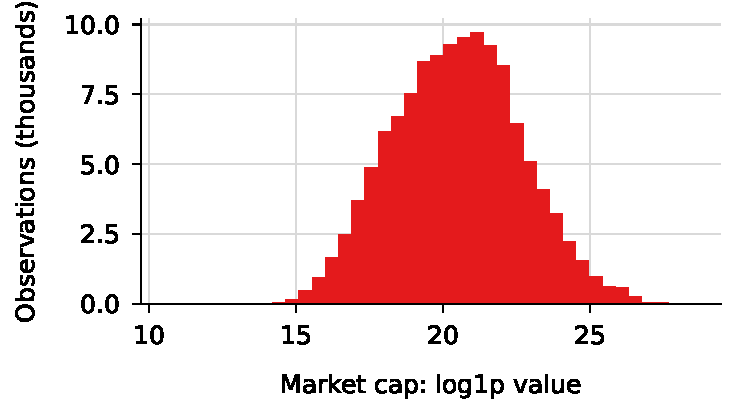
\includegraphics[width=\linewidth]{04_00_market_log_transformation_02_market_cap_usd_log1p.pdf}
        \end{subfigure}
        \par\medskip
        \begin{subfigure}[t]{0.48\textwidth}
                \centering
                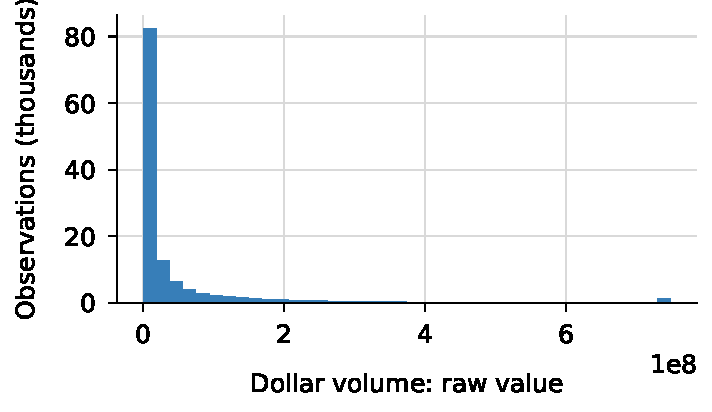
\includegraphics[width=\linewidth]{04_00_market_log_transformation_03_average_daily_dollar_volume_63d_raw.pdf}
        \end{subfigure}
        \hfill
        \begin{subfigure}[t]{0.48\textwidth}
                \centering
                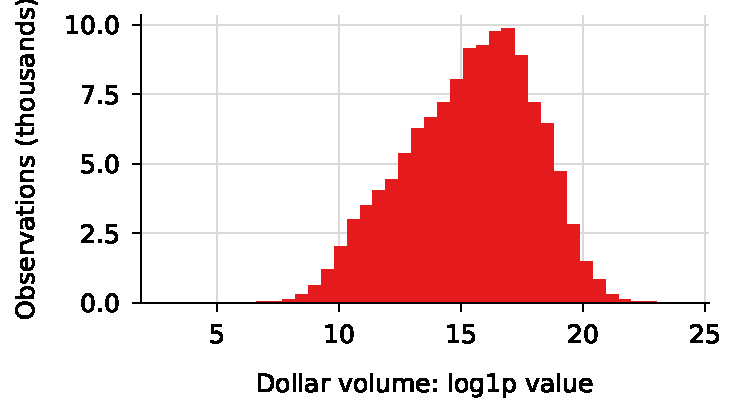
\includegraphics[width=\linewidth]{04_00_market_log_transformation_04_average_daily_dollar_volume_63d_log1p.pdf}
        \end{subfigure}
        \caption[Logarithmic transformations of market scale variables]{Raw and $\log(1+x)$-transformed distributions of market capitalization and average daily dollar volume. Raw panels are capped at their 99th percentiles for display only.}
        \label{fig:log-transformations}
\end{figure}

\begin{figure}[H]
        \centering
        \begin{subfigure}[t]{0.48\textwidth}
                \centering
                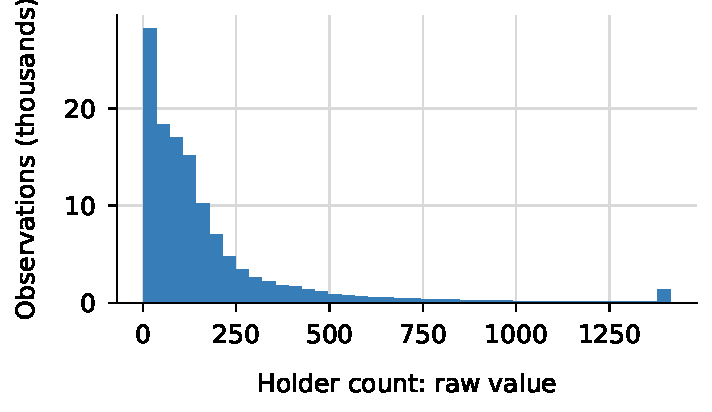
\includegraphics[width=\linewidth]{04_00_ownership_log_transformation_01_institutional_holder_count_raw.pdf}
        \end{subfigure}
        \hfill
        \begin{subfigure}[t]{0.48\textwidth}
                \centering
                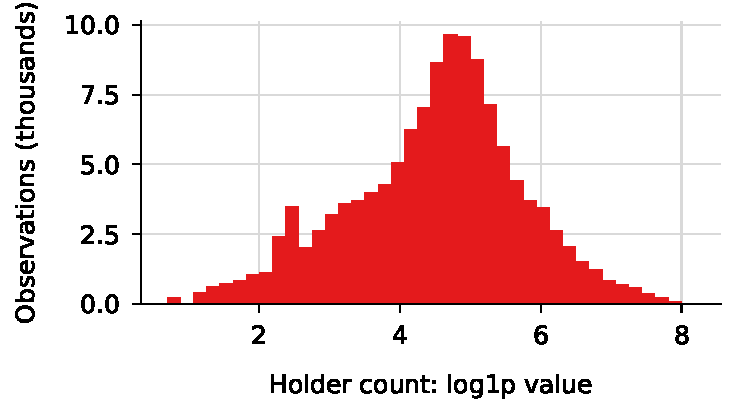
\includegraphics[width=\linewidth]{04_00_ownership_log_transformation_02_institutional_holder_count_log1p.pdf}
        \end{subfigure}
        \par\medskip
        \begin{subfigure}[t]{0.48\textwidth}
                \centering
                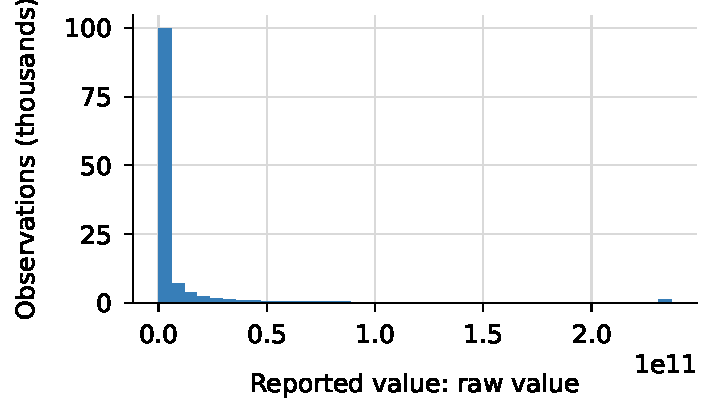
\includegraphics[width=\linewidth]{04_00_ownership_log_transformation_03_total_reported_value_usd_raw.pdf}
        \end{subfigure}
        \hfill
        \begin{subfigure}[t]{0.48\textwidth}
                \centering
                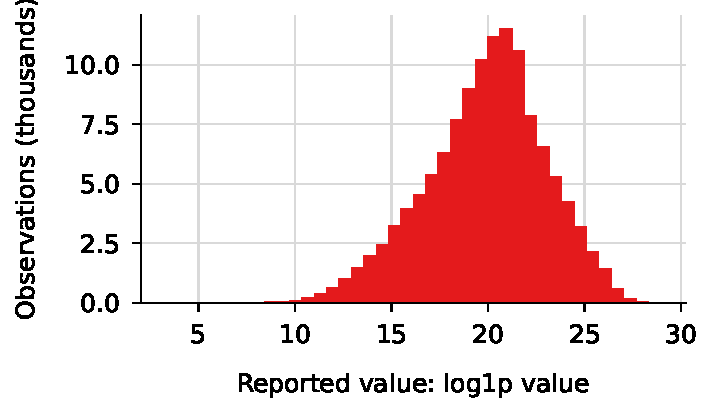
\includegraphics[width=\linewidth]{04_00_ownership_log_transformation_04_total_reported_value_usd_log1p.pdf}
        \end{subfigure}
        \caption[Logarithmic transformations of ownership scale variables]{Raw and $\log(1+x)$-transformed distributions of institutional holder count and total reported institutional value. Raw panels are capped at their 99th percentiles for display only.}
        \label{fig:ownership-log-transformations}
\end{figure}

\noindent
Each retained tabular predictor and graph-node feature is clipped at the 1st and 99th percentiles estimated from the relevant fitting sample, and remaining missing values are replaced by fitting-sample medians. Standardization is applied where required by the model class. The fitted preprocessing parameters are applied unchanged outside the fitting sample, preventing validation or test information from influencing the transformations, clipping bounds, imputation values, or scaling moments.

Before modeling, each network feature is converted to an average-rank percentile within its full quarterly stock universe and scaled from 0 to 1. A feature receives 0.5 if its quarter contains only one valid observation. Ranking is performed before modeling-eligibility restrictions are applied, while missing change features are subsequently handled by fitting-sample median imputation.

\subsection{Strong Feature Correlations}
\label{app:feature_correlations}

Table~\ref{tab:app-strong-feature-correlations} lists every unique feature pair whose absolute mean quarterly Spearman correlation is at least 0.70 in the training sample. Correlations are calculated separately within each quarter and then averaged across quarters, giving every training quarter equal weight. The threshold is used as a compact redundancy diagnostic rather than as an automatic variable-selection rule.

\begingroup
\footnotesize
\setlength{\tabcolsep}{5pt}
\begin{longtable}{>{\raggedright\arraybackslash}p{0.57\textwidth}>{\raggedright\arraybackslash}p{0.25\textwidth}r}
        \caption{Feature pairs with absolute mean quarterly Spearman correlation of at least 0.70}
        \label{tab:app-strong-feature-correlations}                                    \\
        \toprule
        Feature pair                                   & Groups               & $\rho$ \\
        \midrule
        \endfirsthead
        \multicolumn{3}{l}{\footnotesize\itshape Table~\thetable\ continued}           \\
        \toprule
        Feature pair                                   & Groups               & $\rho$ \\
        \midrule
        \endhead
        \midrule
        \multicolumn{3}{r}{\footnotesize\itshape Continued on next page}               \\
        \endfoot
        \bottomrule
        \endlastfoot
        Holder count -- manager-holder share           & Ownership--ownership & 1.000  \\
        Ownership HHI -- top-five ownership share      & Ownership--ownership & 0.963  \\
        Owner-community HHI -- largest community share & Network--network     & 0.958  \\
        Market capitalization -- holder count          & Market--ownership    & 0.954  \\
        Market capitalization -- manager-holder share  & Market--ownership    & 0.954  \\
        Market capitalization -- reported value        & Market--ownership    & 0.943  \\
        Reported value -- manager-holder share         & Ownership--ownership & 0.938  \\
        Holder count -- reported value                 & Ownership--ownership & 0.938  \\
        Dollar volume -- holder count                  & Market--ownership    & 0.937  \\
        Dollar volume -- manager-holder share          & Market--ownership    & 0.937  \\
        Volatility -- downside volatility              & Market--market       & 0.936  \\
        Market capitalization -- dollar volume         & Market--market       & 0.926  \\
        Mean owner weight -- maximum owner weight      & Ownership--ownership & 0.902  \\
        Dollar volume -- reported value                & Market--ownership    & 0.900  \\
        Holder count -- owner-community count          & Ownership--network   & 0.891  \\
        Manager-holder share -- owner-community count  & Ownership--network   & 0.891  \\
        Market capitalization -- owner-community count & Market--network      & 0.844  \\
        Dollar volume -- owner-community count         & Market--network      & 0.834  \\
        Reported value -- owner-community count        & Ownership--network   & 0.831  \\
        Ownership-HHI change -- top-five-share change  & Ownership--ownership & 0.806  \\
        Volatility -- past maximum drawdown            & Market--market       & 0.787  \\
        Downside volatility -- past maximum drawdown   & Market--market       & 0.785  \\
\end{longtable}
\endgroup

\subsection{Redundancy-Based Feature Selection}
\label{app:feature_selection_decisions}

Table~\ref{tab:correlation-feature-selection} summarizes the feature-selection decisions produced by applying the correlation threshold and the interpretability hierarchy described in Section~\ref{sec:feature_engineering}.

\begin{table}[H]
        \centering
        \footnotesize
        \caption{Redundancy-based feature-selection decisions}
        \label{tab:correlation-feature-selection}
        \begin{tabular}{>{\raggedright\arraybackslash}p{0.22\textwidth}>{\raggedright\arraybackslash}p{0.31\textwidth}>{\raggedright\arraybackslash}p{0.36\textwidth}}
                \toprule
                Retained & Excluded                                                                                                                    & Reason \\
                \midrule
                Market capitalization
                         & Dollar volume; holder count; reported value; manager-holder share; owner-community count
                         & Retains the standard measure of firm scale and removes closely related measures of trading and institutional participation.          \\
                Downside volatility
                         & Total volatility
                         & Measures adverse return variation and is more closely aligned with the prediction target.                                            \\
                Ownership HHI
                         & Top-five ownership share
                         & Uses the complete ownership distribution rather than only its largest positions.                                                     \\
                Mean owner portfolio weight
                         & Maximum owner portfolio weight
                         & Represents the stock's importance across all owners rather than one extreme owner.                                                   \\
                Change in ownership HHI
                         & Change in top-five ownership share
                         & Preserves consistency with the retained concentration level.                                                                         \\
                Owner-community HHI
                         & Largest owner-community share
                         & Uses the complete distribution of ownership across communities.                                                                      \\
                \bottomrule
        \end{tabular}
\end{table}

\section{Chronological Sample Allocation}
\label{app:chronological_samples}

The chronological allocation excludes otherwise eligible observations from 2021~Q4 and 2023~Q4. These quarters separate the training sample from validation and validation from test, respectively. At each boundary, the latest target window in the preceding sample closes before the earliest information cutoff in the following sample, ensuring that outcomes used in one sample are fully resolved before the next sample begins.

Figure~\ref{fig:sample-target-distribution} compares the realized distribution of the primary target across the training, validation, and test samples. It documents a rightward shift after the training period, which the fixed chronological evaluation must confront out of sample.

\begin{figure}[H]
        \centering
        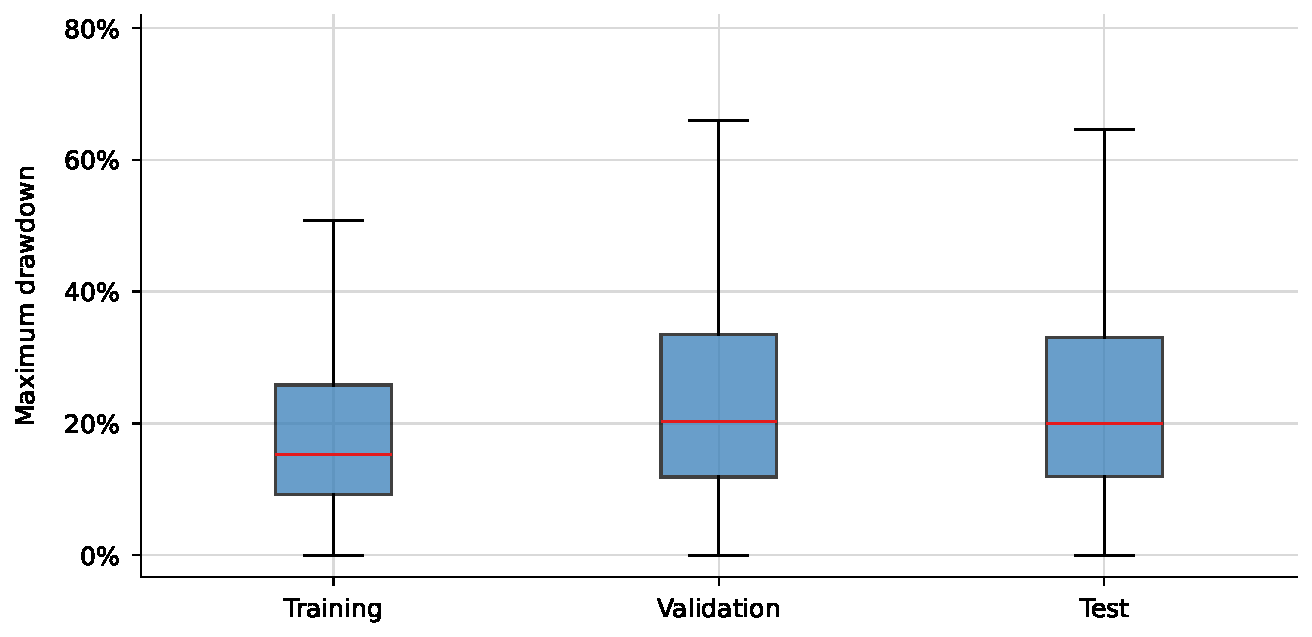
\includegraphics[width=0.75\textwidth]{01_08_target_distribution_boxplot.pdf}
        \caption[Target distribution across the modeling samples]{Distribution of the forward 63-day maximum drawdown target within each chronological sample. Outlier markers are hidden for readability only; all observations are included in the boxplot statistics.}
        \label{fig:sample-target-distribution}
\end{figure}

\section{Graph Neural Network Architectures}
\label{app:gnn_architectures}

All three graph neural networks operate on the quarterly bipartite manager--stock graphs defined in Section~\ref{sec:bipartite_graph}. Each architecture first projects the stock and manager input variables into a common hidden dimension and then passes messages from stocks to managers and from managers back to stocks. The resulting stock representation is mapped to a prediction of forward downside risk. The architectures differ in how neighboring nodes are aggregated and in whether information is carried across quarters.

\subsection{Weighted GraphSAGE}

The GraphSAGE specification uses observed holdings weights to aggregate neighboring representations. Let \(\mathbf{h}^{(0)}_{i,q}\) and \(\mathbf{h}^{(0)}_{m,q}\) denote the initial hidden representations of stock \(i\) and manager \(m\) in quarter \(q\). In the stock-to-manager step, stock messages are weighted by their portfolio weights \(p_{mi,q}\):

\begin{equation}
    \mathbf{h}^{(1)}_{m,q}
    =
    \operatorname{ReLU}
    \left(
        W^{\mathrm{self}}_M\mathbf{h}^{(0)}_{m,q}
        +
        W^{\mathrm{nbr}}_M
        \sum_{i\in\mathcal{N}_q(m)}
        p_{mi,q}\mathbf{h}^{(0)}_{i,q}
    \right).
    \label{eq:weighted_graphsage_manager}
\end{equation}

\noindent
The manager representations are then passed back to stocks using each manager's share \(o_{mi,q}\) of the stock's reported institutional ownership:

\begin{equation}
    \mathbf{g}_{i,q}
    =
    \operatorname{Dropout}
    \left[
    \operatorname{ReLU}
    \left(
        W^{\mathrm{self}}_S\mathbf{h}^{(0)}_{i,q}
        +
        W^{\mathrm{nbr}}_S
        \sum_{m\in\mathcal{N}_q(i)}
        o_{mi,q}\mathbf{h}^{(1)}_{m,q}
    \right)
    \right].
    \label{eq:weighted_graphsage_stock}
\end{equation}

\noindent
The static GraphSAGE prediction is \(\hat{y}_{i,q}=\mathbf{w}_o^{\prime}\mathbf{g}_{i,q}+b_o\). The two sets of observed edge weights determine how strongly each neighbor contributes; the model learns the transformations applied to a node's own representation and to the weighted neighbor aggregate. Each quarterly graph is processed independently.

\subsection{Graph Attention Network}

GAT uses the same two-direction message-passing sequence but learns the relative importance of adjacent nodes. For an edge from source node \(u\) to destination node \(v\), an unnormalized attention score can be represented as

\begin{equation}
    e_{uv,q}
    =
    \operatorname{LeakyReLU}
    \left[
        \mathbf{a}^{\prime}
        \left(
            \Theta_s\mathbf{h}_{u,q}
            \,\Vert\,
            \Theta_d\mathbf{h}_{v,q}
            \,\Vert\,
            \Theta_e\mathbf{e}_{uv,q}
        \right)
    \right],
    \label{eq:gat_attention_score}
\end{equation}

\noindent
where \(\mathbf{e}_{uv,q}\) contains the standardized logarithms of portfolio weight and reported-ownership share. Scores are normalized across the neighbors of the destination node,

\begin{equation}
    \alpha_{uv,q}
    =
    \frac{\exp(e_{uv,q})}
    {\sum_{k\in\mathcal{N}_q(v)}\exp(e_{kv,q})},
    \qquad
    \mathbf{m}_{v,q}
    =
    \sum_{u\in\mathcal{N}_q(v)}
    \alpha_{uv,q}\Theta_s\mathbf{h}_{u,q}.
    \label{eq:gat_attention_weights}
\end{equation}

\noindent
The implementation uses one attention head in each bipartite direction and combines the resulting message with the destination node through a residual update before applying ReLU. Unlike weighted GraphSAGE, GAT is not constrained to treat the reported ownership weights as the final importance assigned to neighboring managers or stocks. It can learn different attention weights from the joint node and edge information, but this additional flexibility also introduces more parameters. Each quarter is again processed independently.

\subsection{Temporal GraphSAGE}

Temporal GraphSAGE first obtains the contemporaneous stock embedding \(\mathbf{g}_{i,q}\) from the weighted GraphSAGE encoder. A gated recurrent unit then combines it with the stock's state from the preceding quarter:

\begin{equation}
    \mathbf{s}_{i,q}
    =
    \operatorname{GRU}
    \left(
        \mathbf{g}_{i,q},
        \mathbf{s}_{i,q-1}
    \right),
    \qquad
    \hat{y}_{i,q}
    =
    \mathbf{w}_o^{\prime}\mathbf{s}_{i,q}+b_o.
    \label{eq:temporal_graphsage}
\end{equation}

\noindent
This architecture therefore combines the current ownership network with information retained from previous quarterly snapshots. The preceding state is reset to zero when a stock was absent from the immediately preceding quarter. Purged snapshots update the recurrent state but do not contribute to the training loss.

In summary, weighted GraphSAGE aggregates current neighbors using observed ownership weights, GAT learns the relative importance of current neighbors, and temporal GraphSAGE adds memory of how each stock's graph representation evolves through time.

\section{Model Settings and Selection Rules}
\label{app:model_specifications}

Table~\ref{tab:model-specifications} reports the fixed model settings, controlled validation-stage refinements, and staged selection rules used in the predictive analysis. The common project seed is 42. Ridge is deterministic under the stated specification; the seed is applied to XGBoost and to the Python, NumPy, and PyTorch random-number generators used for graph-model estimation. PyTorch deterministic algorithms are enabled for the GNNs.

\begingroup
\scriptsize
\setlength{\tabcolsep}{4pt}
\renewcommand{\arraystretch}{1.15}
\begin{longtable}{>{\raggedright\arraybackslash}p{0.19\textwidth}>{\raggedright\arraybackslash}p{0.24\textwidth}>{\raggedright\arraybackslash}p{0.47\textwidth}}
        \caption{Predictive-model specifications and selection rules}
        \label{tab:model-specifications}                                                                                                                                                                                                                                                                                                                                                                                                                                                                                                          \\
        \toprule
        Model & Component                                                                                                                                                                                                                                                                                                                                                                                                                                                                                                         & Specification \\
        \midrule
        \endfirsthead
        \toprule
        Model & Component                                                                                                                                                                                                                                                                                                                                                                                                                                                                                                         & Specification \\
        \midrule
        \endhead
        \bottomrule
        \endfoot
        No-information benchmark
              & Forecast
              & Constant equal to the fitting-sample mean target: the training mean for validation and the combined training--validation mean for the final test comparison.                                                                                                                                                                                                                                                                                                                                                                      \\
        All fitted models
              & Selection rule
              & Validation MAE is the primary quantitative criterion. When MAE differences are negligible, RMSE, $R^2$, mean quarterly Spearman correlation, convergence, and model complexity are used to prefer the more stable and parsimonious specification.                                                                                                                                                                                                                                                                             \\
        Modeling ladder
              & Staged selection
              & First, the three nested feature sets are compared separately within Ridge and XGBoost under common model-specific settings. One feature set is retained within each class, using parsimony when validation performance is materially similar. Second, the retained XGBoost specification is refined through a controlled comparison while Ridge remains fixed. Third, the three GNN architectures are compared under a common configuration and only the strongest architecture is refined. The retained Ridge, XGBoost, and GNN specifications then enter the final validation comparison.                                                       \\
        Finalists
              & Refitting
              & The feature sets, hyperparameters, and validation-selected number of boosting rounds or training epochs are held fixed while all three finalists are re-estimated on the combined training and validation samples. They are evaluated once on the test sample to assess generalization without reopening model selection.                                                                                                                                                                                                      \\
        Ridge
              & Estimator
              & Linear regression with an $L_2$ penalty; predictors are standardized using fitting-sample moments.                                                                                                                                                                                                                                                                                                                                                                                                                              \\
        Ridge
              & Penalty
              & All feature-set and finalist comparisons use the prespecified value $\alpha=1$; no separate Ridge tuning stage is performed.                                                                                                                                                                                                                                                                                                                                                                                                 \\
        XGBoost
              & Training objective
              & Squared-error regression objective (\texttt{reg:squarederror}); validation MAE is the primary evaluation and selection metric. Trees are constructed using the histogram method.                                                                                                                                                                                                                                                                                                                                                  \\
        XGBoost
              & Initial settings
              & The feature-set comparison permits at most 1,000 boosting rounds and uses maximum depth 3, minimum child weight 1, row subsampling 0.8, learning rate 0.05, and column subsampling 0.8. Validation MAE is monitored with early-stopping patience of 30 rounds.                                                                                                                                                                                                                                                                         \\
        XGBoost
              & Controlled refinement
              & The retained specification is compared under three configurations: $(\eta,\text{depth})\in\{(0.05,3),(0.10,3),(0.10,4)\}$. Minimum child weight remains 1, row and column subsampling remain 0.8, and each configuration permits at most 1,000 rounds with early-stopping patience of 30. The depth-three, $\eta=0.10$ configuration is retained at its validation-selected round because it matches the validation performance of the alternatives with faster convergence and less complexity than the deeper model. \\
        All GNNs
              & Node and edge preprocessing
              & Stock nodes use the seven retained market and five retained ownership features. Manager nodes use portfolio value, security count, largest position weight, and portfolio HHI. Market capitalization, manager portfolio value, and manager security count receive $\log(1+x)$ transformations. Node features are clipped, median-imputed, and standardized using the fitting sample. For GAT, the logarithms of portfolio weight and reported-ownership share are standardized using fitting-sample edge moments.                 \\
        All GNNs
              & Initial comparison
              & GraphSAGE, GAT, and temporal GraphSAGE are first compared using a common hidden dimension of 16, dropout of 0.20, learning rate of 0.001, and weight decay of 0.0001. Each architecture uses one stock-to-manager and one manager-to-stock message-passing stage, ReLU activation, and a scalar linear output layer.                                                                                                                                                                                                                  \\
        All GNNs
              & Estimation
              & $L_1$ training loss and Adam optimizer; at most 50 epochs; validation MAE evaluated after every epoch; early-stopping patience 5 with minimum improvement 0.0001. The checkpoint with the lowest validation MAE is retained.                                                                                                                                                                                                                                                                                                      \\
        Selected GNN
              & Controlled refinement
              & The retained Temporal GraphSAGE architecture is evaluated under the base configuration $(16,0.20,0.001)$ and four variants $(16,0.20,0.010)$, $(32,0.20,0.001)$, $(32,0.30,0.001)$, and $(64,0.30,0.001)$, where each tuple gives hidden dimension, dropout, and learning rate. Weight decay remains 0.0001 and the same early-stopping rule is used. The configuration $(32,0.20,0.001)$ is retained at epoch 28.                                                                                                                         \\
        GraphSAGE
              & Aggregation
              & Weighted neighbour aggregation in both bipartite directions. Stock messages entering a manager are weighted by portfolio weight; manager messages entering a stock are weighted by reported-ownership share. Each update combines separate linear transformations of the node's current representation and its weighted neighbour aggregate.                                                                                                                                                                                      \\
        GAT
              & Attention
              & Two single-head bipartite attention layers, one in each direction, with no self-loops, no concatenation across heads, residual updates, and two edge attributes: the standardized logarithms of portfolio weight and reported-ownership share.                                                                                                                                                                                                                                                                                  \\
        Temporal GraphSAGE
              & Recurrent state
              & The contemporaneous GraphSAGE stock embedding and the stock's preceding-quarter hidden state enter a gated recurrent unit. The prior state is reset to zero when the stock was absent from the immediately preceding quarter. Purged snapshots update states but contribute no training loss.                                                                                                                                                                                                                                     \\
\end{longtable}
\endgroup


\chapter{Supplementary Results}
\label{chap:results_appendix}
This appendix contains supplementary empirical diagnostics referenced in Chapter~\ref{chap:results} but not required for the main sequence of results.

\section{Ridge Feature-Set Diagnostics}
\label{app:linear_feature_set_diagnostics}

Figure~\ref{fig:app-ridge-feature-deciles} compares validation errors across realized-drawdown deciles for the three Ridge feature sets. The three specifications have nearly identical error profiles. Errors are lowest in the middle of the realized-drawdown distribution and rise sharply in the most severe drawdown decile. The additional ownership and network features therefore do not materially change where the linear model succeeds or fails.

\begin{figure}[!htbp]
    \centering
    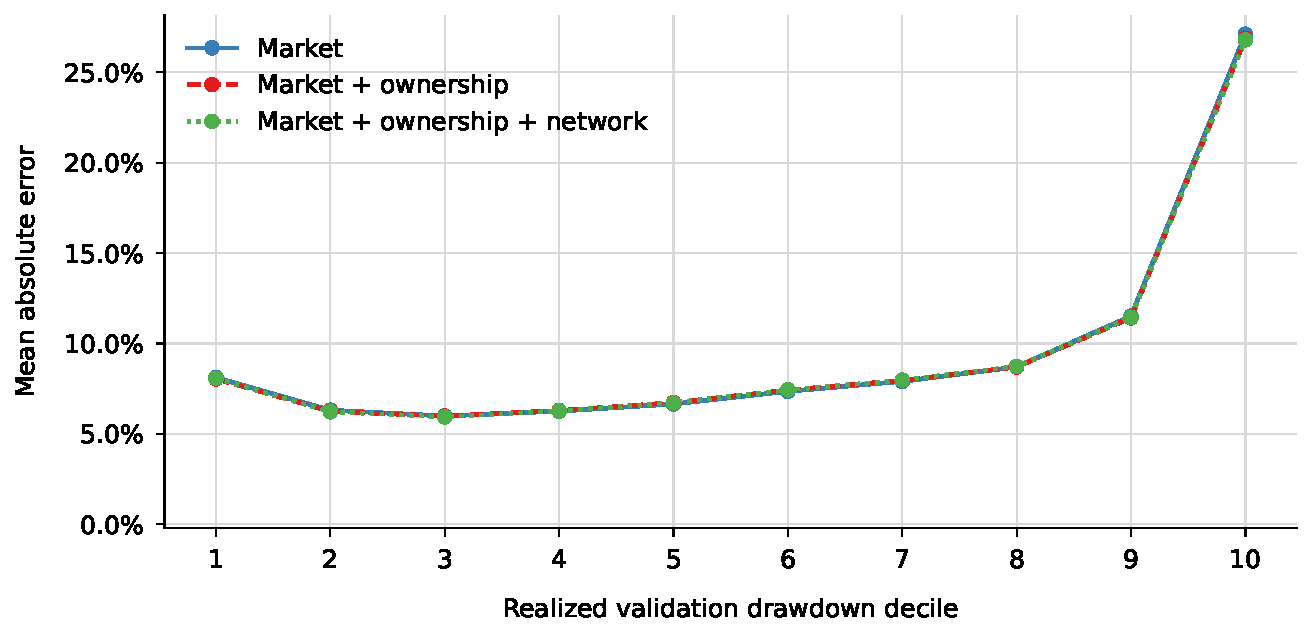
\includegraphics[width=0.82\textwidth]{04_01_ridge_validation_mae_by_realized_drawdown_decile.pdf}
    \caption[Ridge validation errors across realized drawdown deciles]{Validation MAE across realized-drawdown deciles for Ridge estimated using MKT, MKT~+~OWN, and MKT~+~OWN~+~NTW features.}
    \label{fig:app-ridge-feature-deciles}
\end{figure}

\section{XGBoost Feature-Set Diagnostics}
\label{app:nonlinear_feature_set_diagnostics}

Figure~\ref{fig:app-xgboost-feature-deciles} compares validation errors across realized-drawdown deciles for the three XGBoost feature sets. The nearly overlapping profiles show that adding ownership and network variables does not materially alter the distribution of prediction errors. Errors remain lowest in the middle of the realized-drawdown distribution and increase sharply for the most severe drawdowns.

\begin{figure}[!htbp]
    \centering
    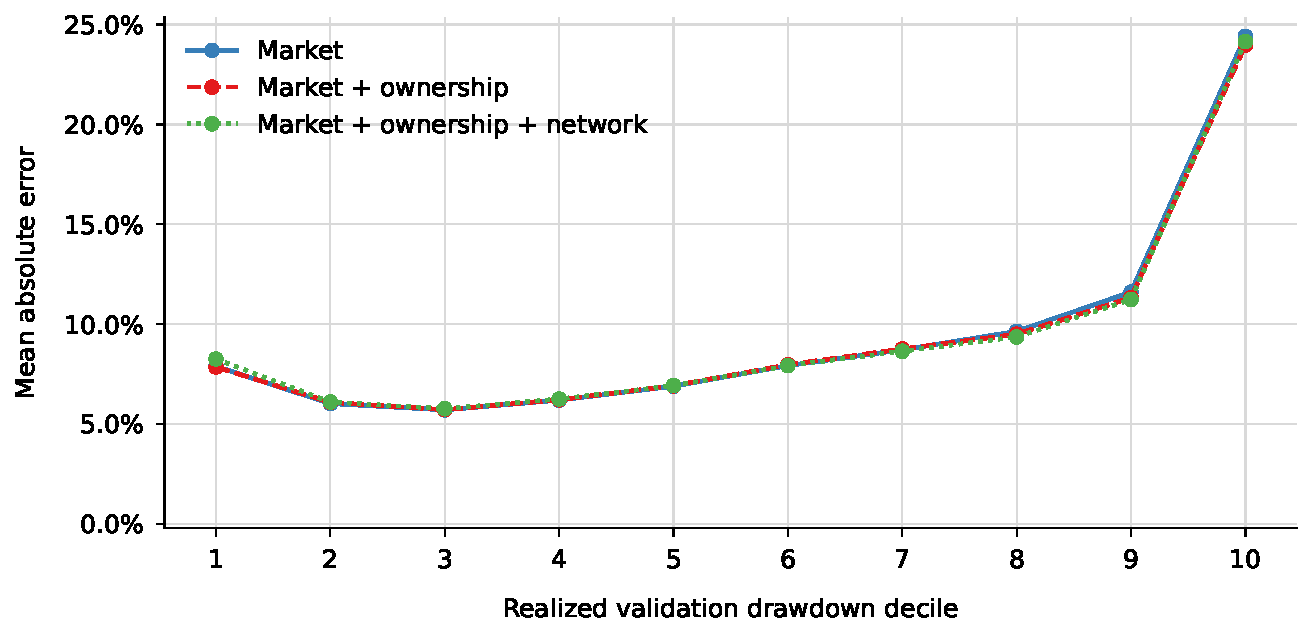
\includegraphics[width=0.82\textwidth]{04_02_xgboost_validation_mae_by_realized_drawdown_decile.pdf}
    \caption[XGBoost validation errors across realized drawdown deciles]{Validation MAE across realized-drawdown deciles for XGBoost estimated using MKT, MKT~+~OWN, and MKT~+~OWN~+~NTW features.}
    \label{fig:app-xgboost-feature-deciles}
\end{figure}

\section{XGBoost Tuning Details}
\label{app:xgboost_tuning_details}

Table~\ref{tab:selected-xgboost-configuration} reports the complete configuration retained after the controlled tuning comparison in Section~\ref{sec:xgboost_tuning_results}.

\begin{table}[!htbp]
\centering
\footnotesize
\caption{Selected market-only XGBoost configuration.}
\label{tab:selected-xgboost-configuration}
\begin{tabular}{lr}
\toprule
Parameter & Value \\
\midrule
Learning rate & 0.10 \\
Maximum depth & 3 \\
Minimum child weight & 1 \\
Row subsample & 0.80 \\
Column subsample & 0.80 \\
Maximum boosting rounds & 1,000 \\
Early-stopping patience & 30 rounds \\
Training objective & Squared error \\
Validation metric & MAE \\
Selected boosting round & 90 \\
Training MAE & 0.0836 \\
Validation MAE & 0.0951 \\
\bottomrule
\end{tabular}
\end{table}


\section{GNN Architecture Details}
\label{app:gnn_architecture_details}

The three architectures are initially estimated using a common hidden dimension of 16, dropout of 0.20, learning rate of 0.001, and weight decay of 0.0001. Figure~\ref{fig:app-gnn-base-learning-curves} reports their individual training and validation learning curves.

\begin{figure}[!htbp]
    \centering
    \begin{subfigure}[t]{0.48\textwidth}
        \centering
        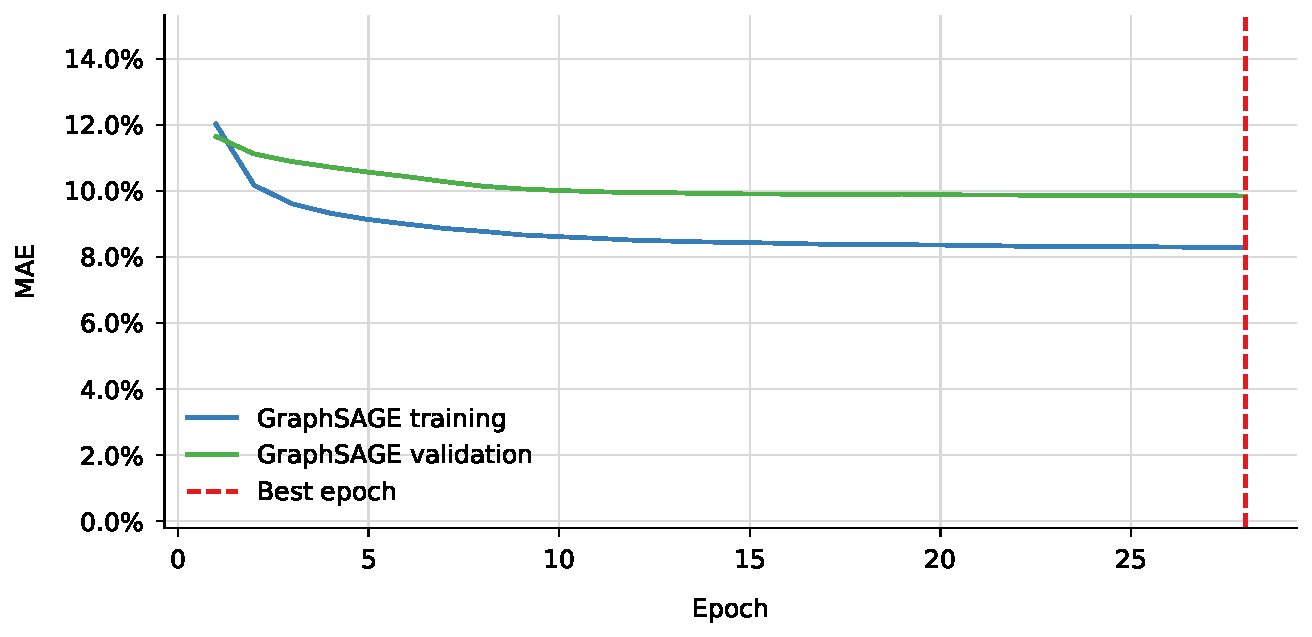
\includegraphics[width=\linewidth]{04_04_graphsage_learning_curve.pdf}
        \caption{GraphSAGE.}
    \end{subfigure}
    \hfill
    \begin{subfigure}[t]{0.48\textwidth}
        \centering
        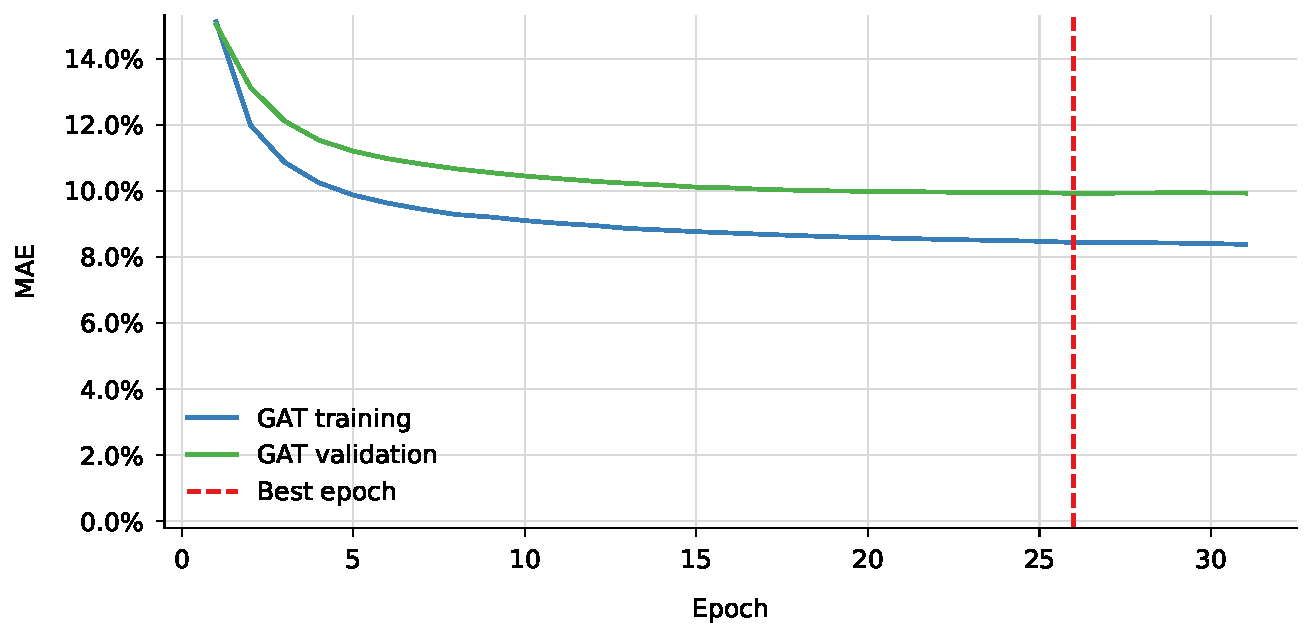
\includegraphics[width=\linewidth]{04_04_gat_learning_curve.pdf}
        \caption{GAT.}
    \end{subfigure}

    \medskip

    \begin{subfigure}[t]{0.48\textwidth}
        \centering
        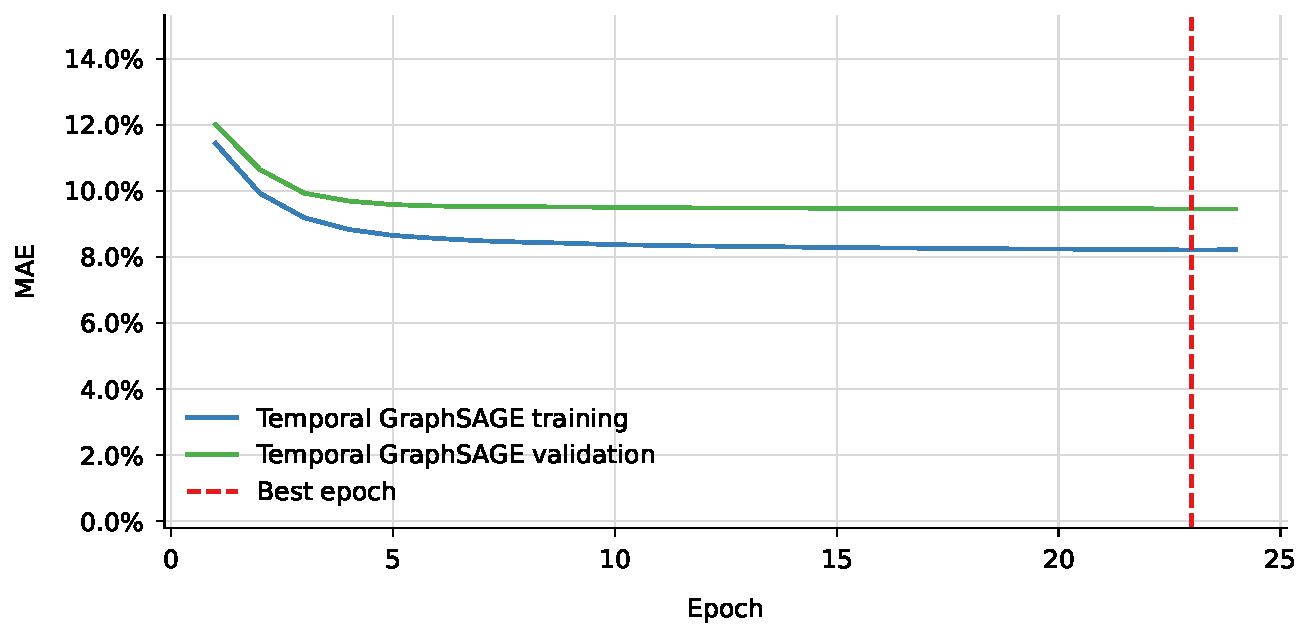
\includegraphics[width=\linewidth]{04_04_temporal_graphsage_learning_curve.pdf}
        \caption{Temporal GraphSAGE.}
    \end{subfigure}
    \caption{Learning curves for the three GNN architectures under the common initial configuration.}
    \label{fig:app-gnn-base-learning-curves}
\end{figure}

\section{Temporal GraphSAGE Tuning Details}
\label{app:gnn_tuning_details}

Table~\ref{tab:selected-temporal-graphsage-configuration} reports the complete configuration retained after the tuning comparison in Section~\ref{sec:temporal_graphsage_tuning}. Figure~\ref{fig:app-temporal-graphsage-tuning-curves} reports the individual learning curves for the four tuned variants.

\begin{table}[!htbp]
\centering
\footnotesize
\caption{Selected Temporal GraphSAGE configuration.}
\label{tab:selected-temporal-graphsage-configuration}
\begin{tabular}{lr}
\toprule
Parameter & Value \\
\midrule
Architecture & Temporal GraphSAGE \\
Hidden dimension & 32 \\
Learning rate & 0.001 \\
Dropout & 0.20 \\
Weight decay & 0.0001 \\
Optimizer & Adam \\
Training loss & MAE \\
Maximum epochs & 50 \\
Early-stopping patience & 5 epochs \\
Minimum improvement & 0.0001 \\
Selected epoch & 28 \\
Training MAE & 0.0813 \\
Validation MAE & 0.0941 \\
\bottomrule
\end{tabular}
\end{table}


\begin{figure}[!htbp]
    \centering
    \begin{subfigure}[t]{0.48\textwidth}
        \centering
        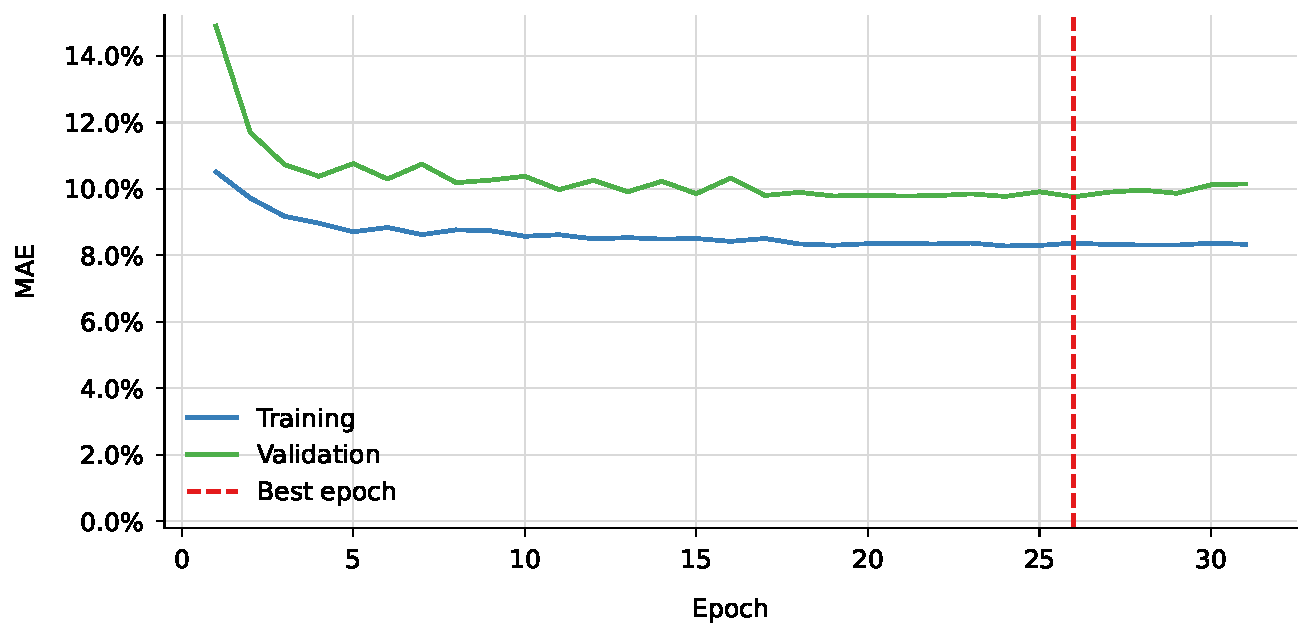
\includegraphics[width=\linewidth]{04_04_temporal_graphsage_hidden_16_lr_0010_learning_curve.pdf}
        \caption{Hidden 16; learning rate 0.010; dropout 0.20.}
    \end{subfigure}
    \hfill
    \begin{subfigure}[t]{0.48\textwidth}
        \centering
        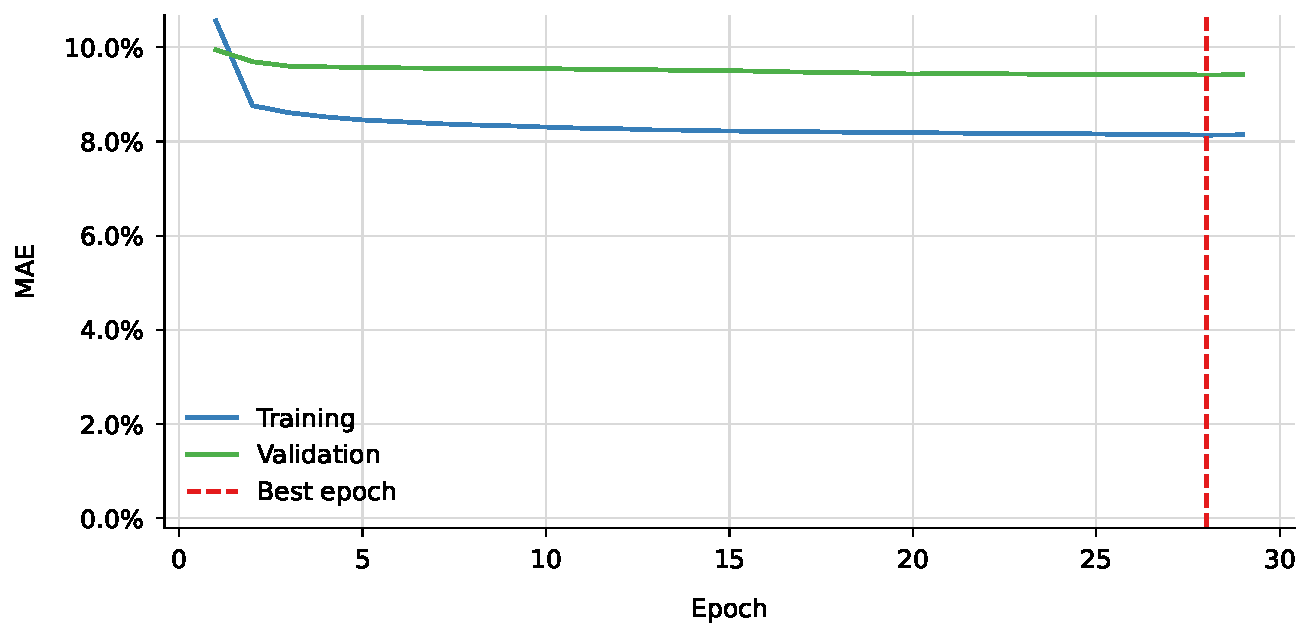
\includegraphics[width=\linewidth]{04_04_temporal_graphsage_hidden_32_learning_curve.pdf}
        \caption{Hidden 32; learning rate 0.001; dropout 0.20.}
    \end{subfigure}

    \medskip

    \begin{subfigure}[t]{0.48\textwidth}
        \centering
        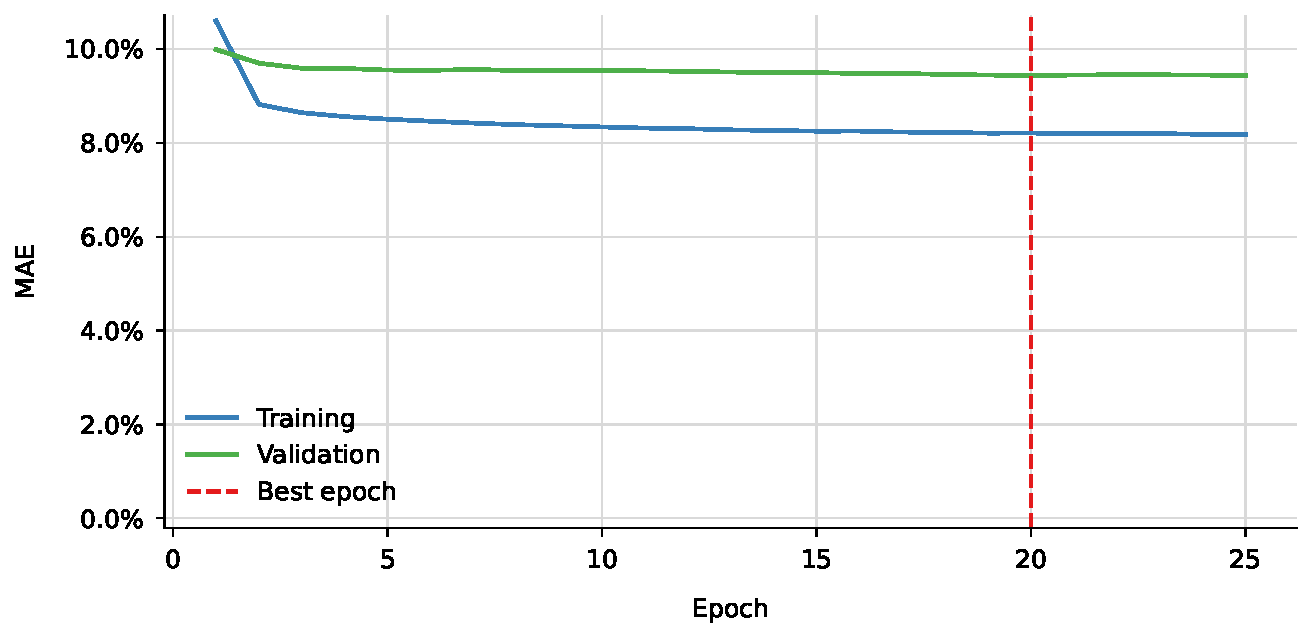
\includegraphics[width=\linewidth]{04_04_temporal_graphsage_hidden_32_dropout_030_learning_curve.pdf}
        \caption{Hidden 32; learning rate 0.001; dropout 0.30.}
    \end{subfigure}
    \hfill
    \begin{subfigure}[t]{0.48\textwidth}
        \centering
        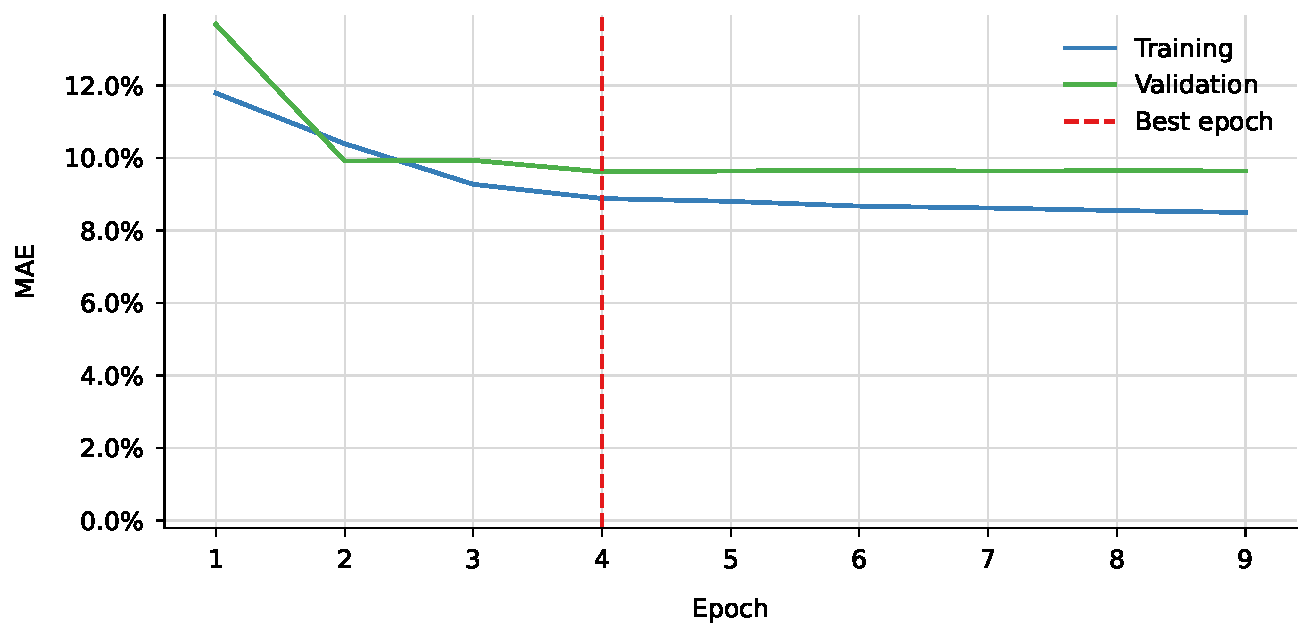
\includegraphics[width=\linewidth]{04_04_temporal_graphsage_hidden_64_dropout_030_learning_curve.pdf}
        \caption{Hidden 64; learning rate 0.001; dropout 0.30.}
    \end{subfigure}
    \caption{Learning curves for the four tuned Temporal GraphSAGE configurations.}
    \label{fig:app-temporal-graphsage-tuning-curves}
\end{figure}

\section{XGBoost Interpretation Diagnostics}
\label{app:model_interpretation_details}

Figure~\ref{fig:app-xgboost-shap-dependence} reports SHAP dependence plots for the three most influential predictors. Higher downside volatility and larger past maximum drawdown are associated with larger positive contributions to predicted downside risk, whereas larger market capitalization generally contributes negatively. These patterns describe the fitted model and should not be interpreted as causal effects.

\begin{figure}[!htbp]
    \centering
    \begin{subfigure}[t]{0.48\textwidth}
        \centering
        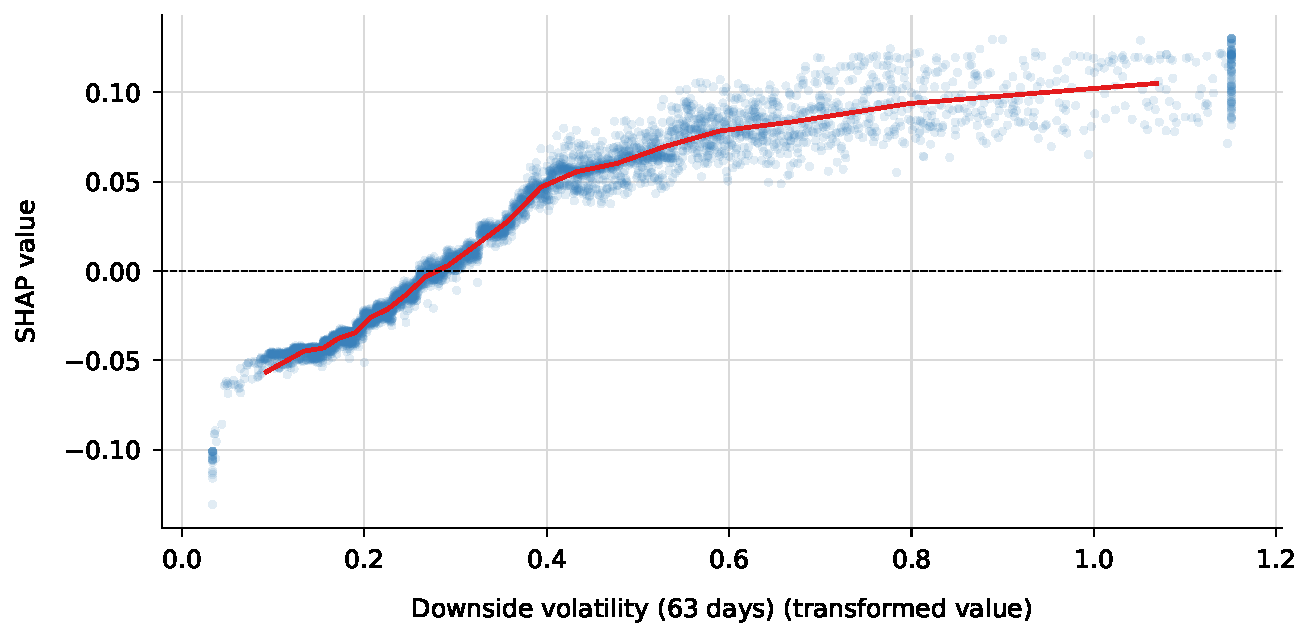
\includegraphics[width=\linewidth]{04_11_xgboost_shap_dependence_1_downside_volatility_63_days.pdf}
        \caption{Downside volatility.}
    \end{subfigure}
    \hfill
    \begin{subfigure}[t]{0.48\textwidth}
        \centering
        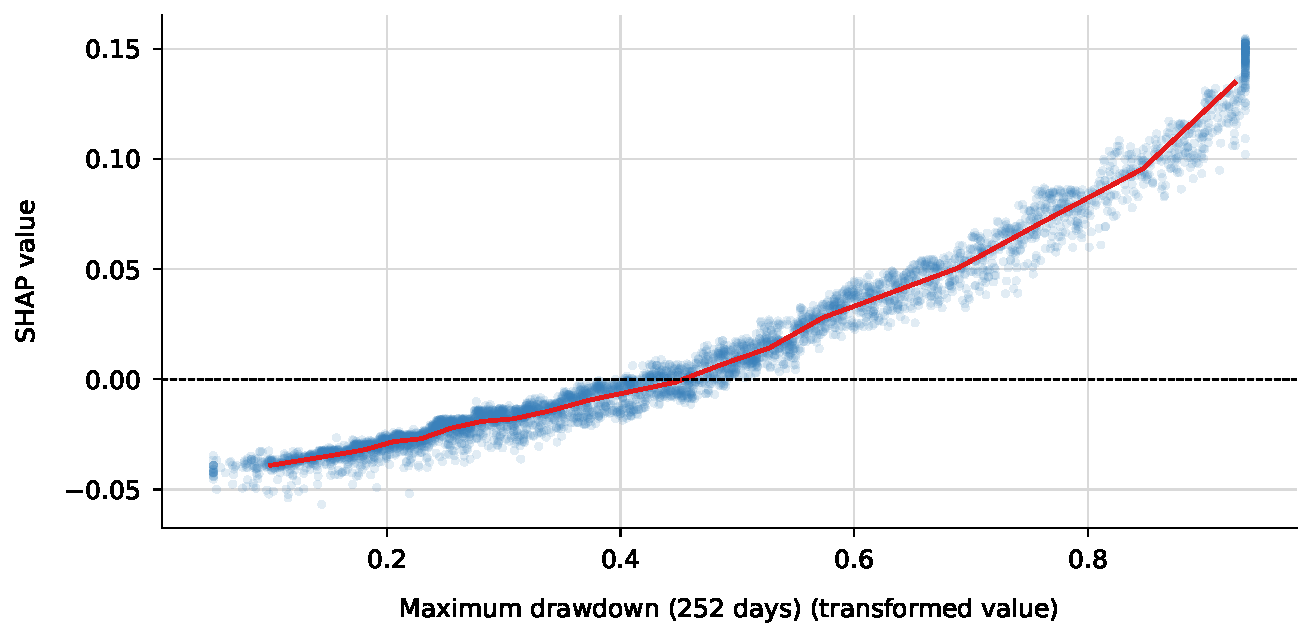
\includegraphics[width=\linewidth]{04_11_xgboost_shap_dependence_2_maximum_drawdown_252_days.pdf}
        \caption{Past maximum drawdown.}
    \end{subfigure}

    \medskip

    \begin{subfigure}[t]{0.48\textwidth}
        \centering
        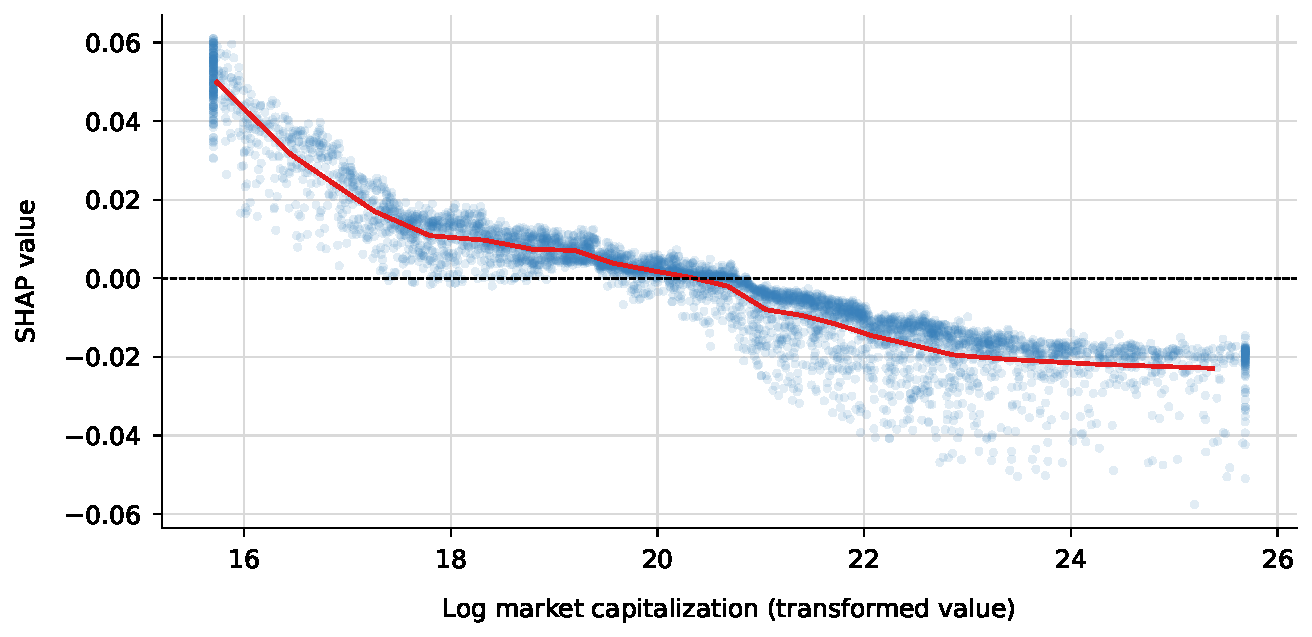
\includegraphics[width=\linewidth]{04_11_xgboost_shap_dependence_3_log_market_capitalization.pdf}
        \caption{Market capitalization.}
    \end{subfigure}
    \caption[SHAP dependence patterns for the leading predictors]{SHAP contributions across the transformed values of the three most influential predictors in the selected XGBoost model. The fitted lines summarize the corresponding dependence patterns.}
    \label{fig:app-xgboost-shap-dependence}
\end{figure}

\noindent
Figure~\ref{fig:app-xgboost-quarterly-shap} compares normalized SHAP importance across test quarters. The feature ordering is highly stable over time, showing that the selected model relies on a consistent set of predictors rather than changing its principal drivers from one quarter to another.

\begin{figure}[!htbp]
    \centering
    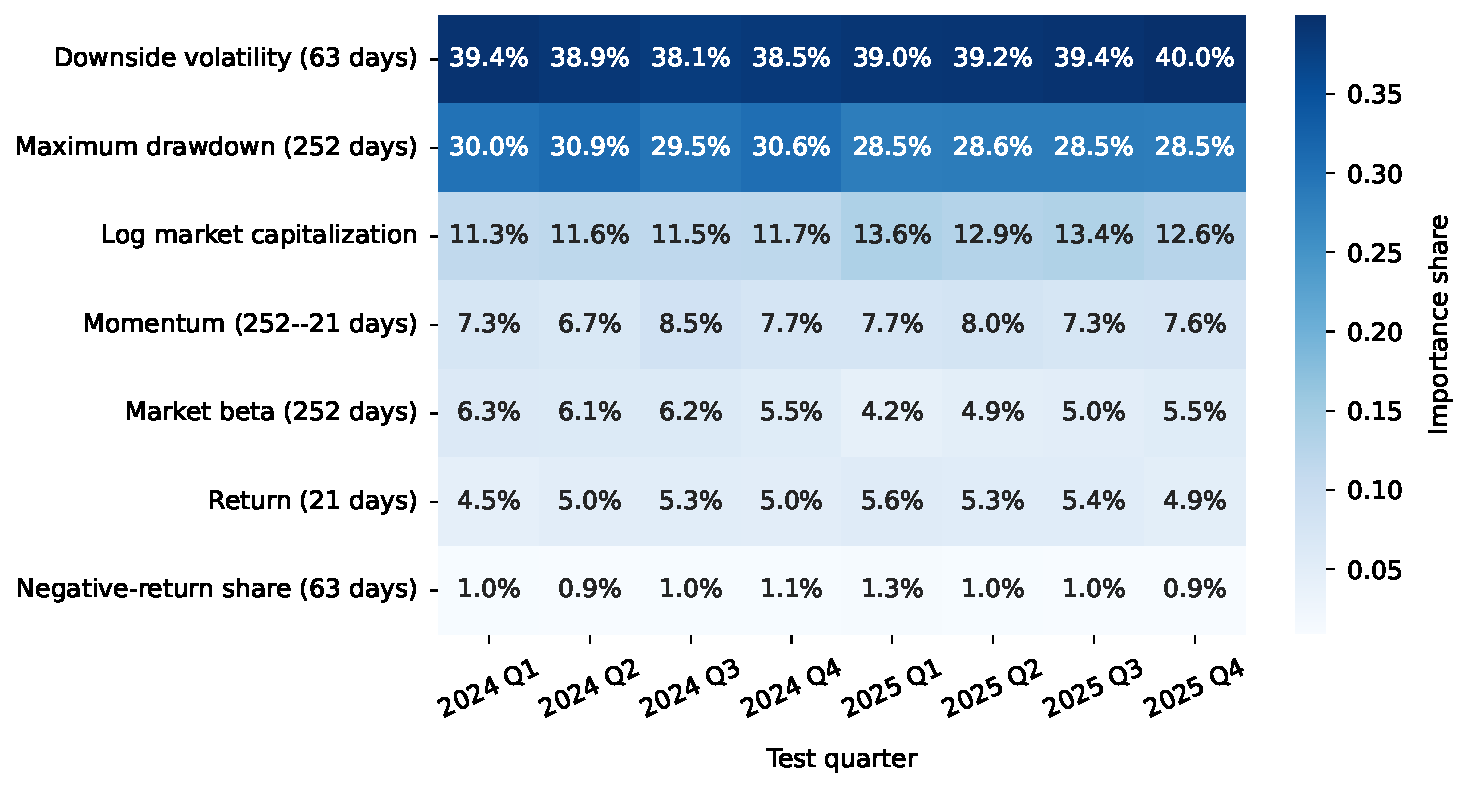
\includegraphics[width=0.9\textwidth]{04_11_xgboost_quarterly_shap_importance_heatmap.pdf}
    \caption[Feature-importance stability across test quarters]{Normalized mean absolute SHAP importance by test quarter for the selected XGBoost model. Each column sums to one, and features are ordered by their average importance.}
    \label{fig:app-xgboost-quarterly-shap}
\end{figure}

\section{Held-Out Model Comparison Diagnostics}
\label{app:quarterly_test_performance}

Figure~\ref{fig:finalist-test-deciles} compares the three finalists across realized-drawdown deciles. Their error profiles remain close through the first nine deciles and rise sharply in the tenth, showing that all three models have greater difficulty estimating the magnitude of the most severe downside outcomes.

\begin{figure}[!htbp]
    \centering
    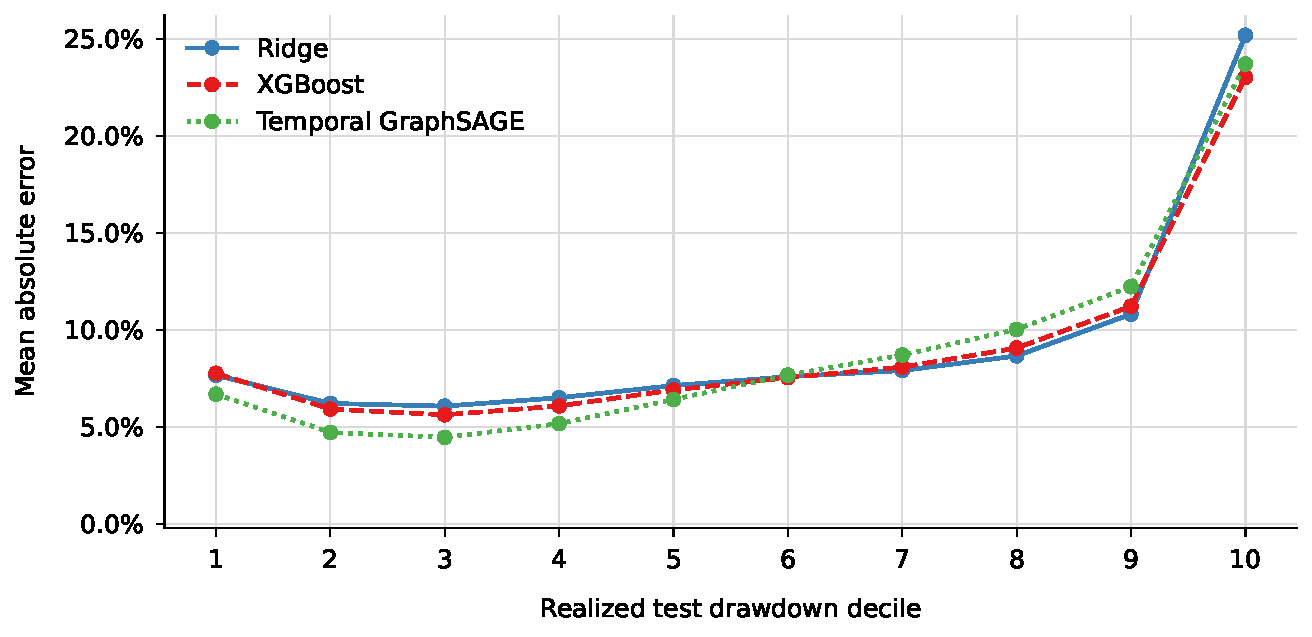
\includegraphics[width=0.82\textwidth]{04_08_test_mae_by_realized_drawdown_decile.pdf}
    \caption[Held-out errors across realized drawdown deciles]{Test MAE across realized-drawdown deciles for the three frozen finalist models.}
    \label{fig:finalist-test-deciles}
\end{figure}

\noindent
Figure~\ref{fig:app-finalist-quarterly-performance} reports the MAE and within-quarter Spearman correlation of the three frozen finalist models in each test quarter. Quarterly MAE varies across the test period, while within-quarter rank correlations remain consistently positive. This indicates that the models' ability to rank stocks is more stable than their ability to estimate the magnitude of realized downside across periods.

\begin{figure}[!htbp]
    \centering
    \begin{subfigure}[t]{0.48\textwidth}
        \centering
        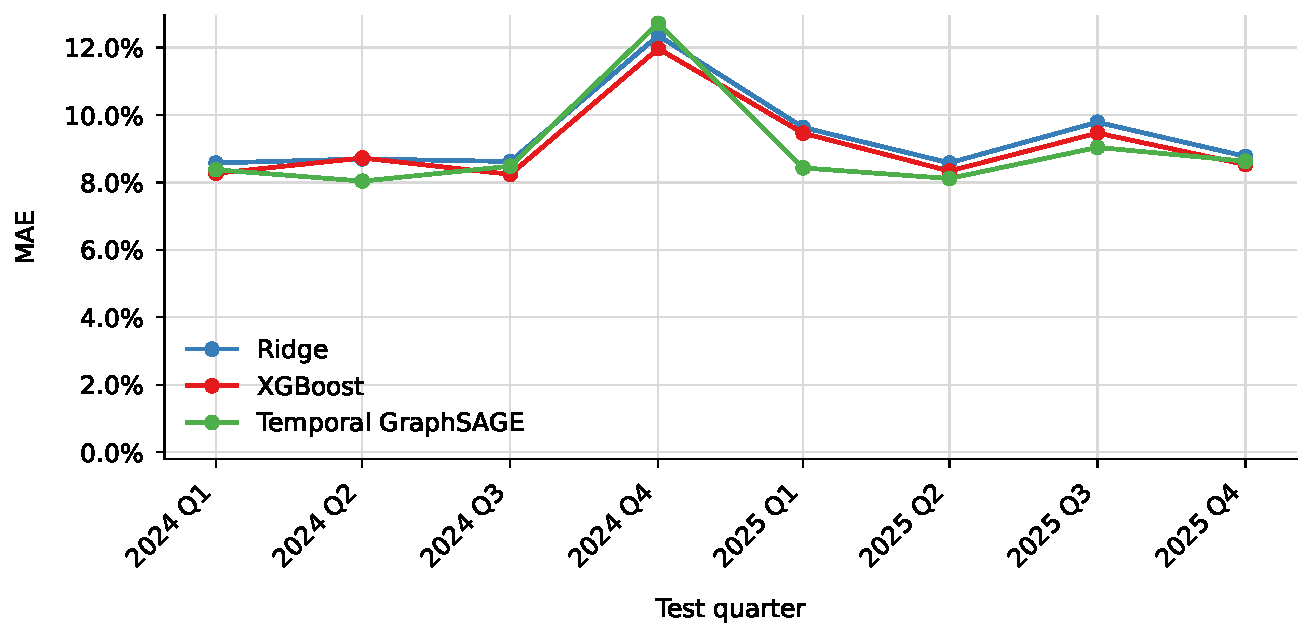
\includegraphics[width=\linewidth]{04_08_quarterly_test_mae_finalists.pdf}
        \caption{Quarterly MAE.}
        \label{fig:app-finalist-quarterly-mae}
    \end{subfigure}
    \hfill
    \begin{subfigure}[t]{0.48\textwidth}
        \centering
        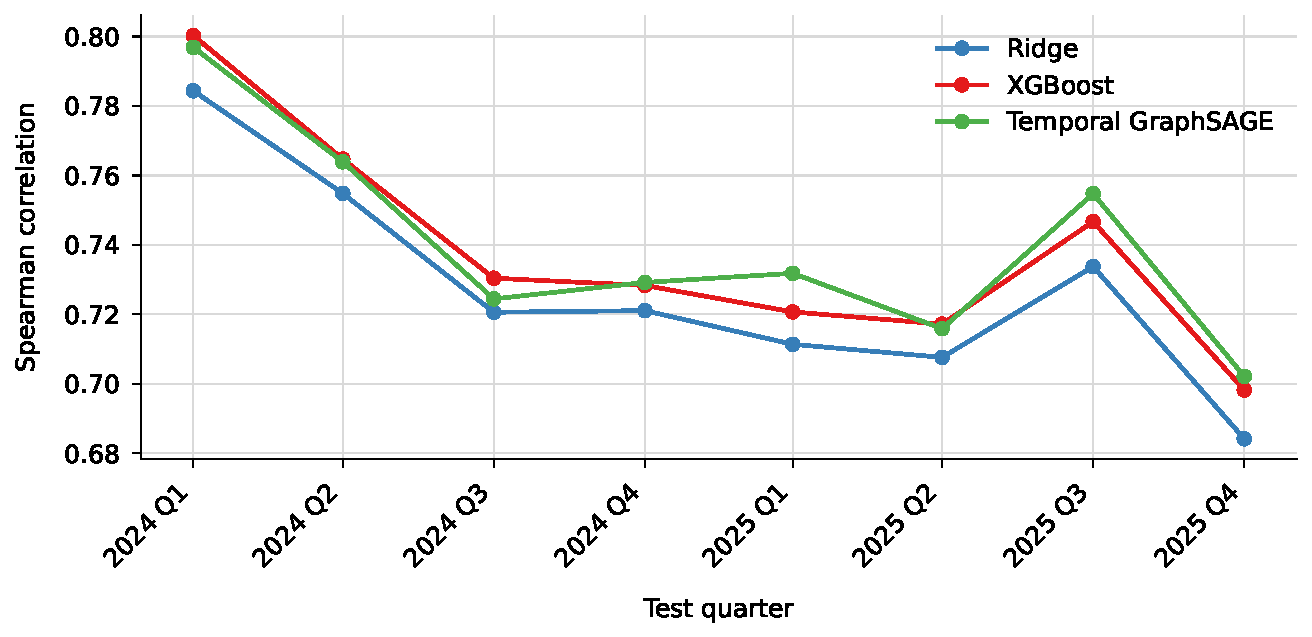
\includegraphics[width=\linewidth]{04_08_quarterly_test_spearman_finalists.pdf}
        \caption{Quarterly rank correlation.}
        \label{fig:app-finalist-quarterly-spearman}
    \end{subfigure}
    \caption[Quarterly held-out performance of the finalist models]{MAE and Spearman rank correlation by test quarter for the three frozen finalist models.}
    \label{fig:app-finalist-quarterly-performance}
\end{figure}

\section{Firm-Size Error Diagnostic}
\label{app:firm_size_errors}

Figure~\ref{fig:app-xgboost-mae-size} reports the selected model's held-out MAE across within-quarter market-capitalization quintiles. Errors are larger among smaller stocks, although this supplementary relationship is not subjected to a separate robustness analysis.

\begin{figure}[!htbp]
    \centering
    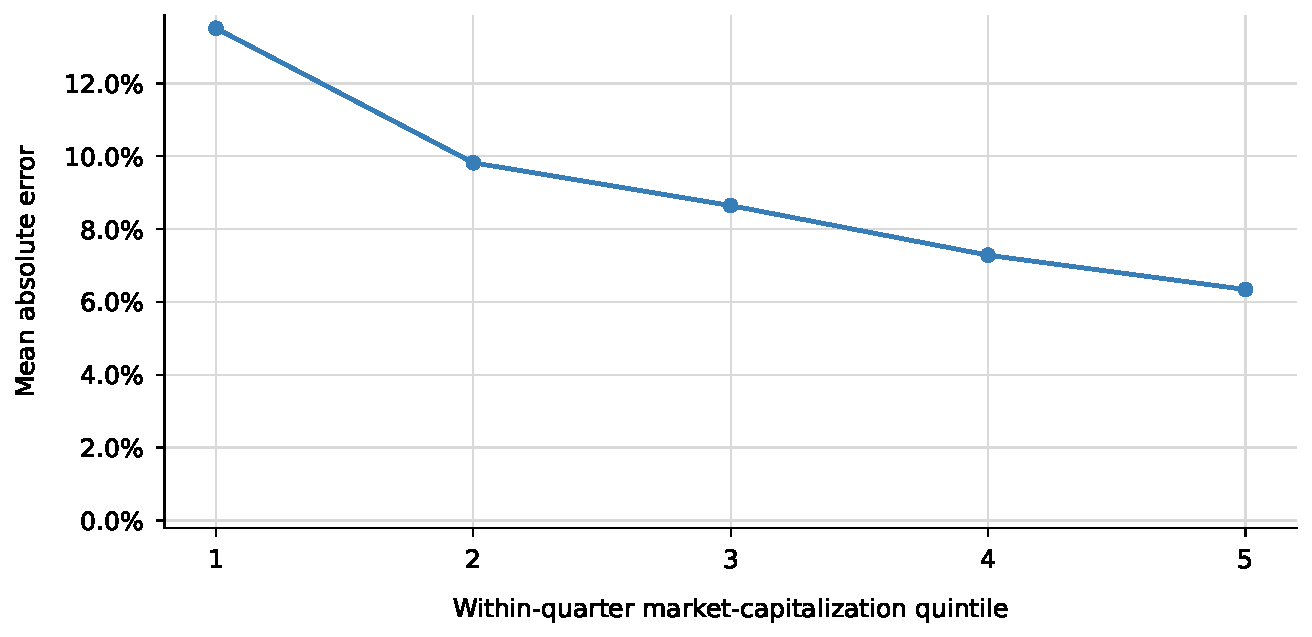
\includegraphics[width=0.72\textwidth]{04_09_xgboost_test_mae_by_size.pdf}
    \caption[Selected-model errors by firm size]{Held-out MAE across within-quarter market-capitalization quintiles.}
    \label{fig:app-xgboost-mae-size}
\end{figure}

\section{Predictive Robustness Diagnostics}
\label{app:predictive_robustness_stability}

Figure~\ref{fig:app-predictive-robustness-deciles} reports standardized realized outcomes across predicted-risk deciles. The monotonic or near-monotonic profiles show that the model's ranking ability extends across downside-risk definitions and horizons.

\begin{figure}[!htbp]
    \centering
    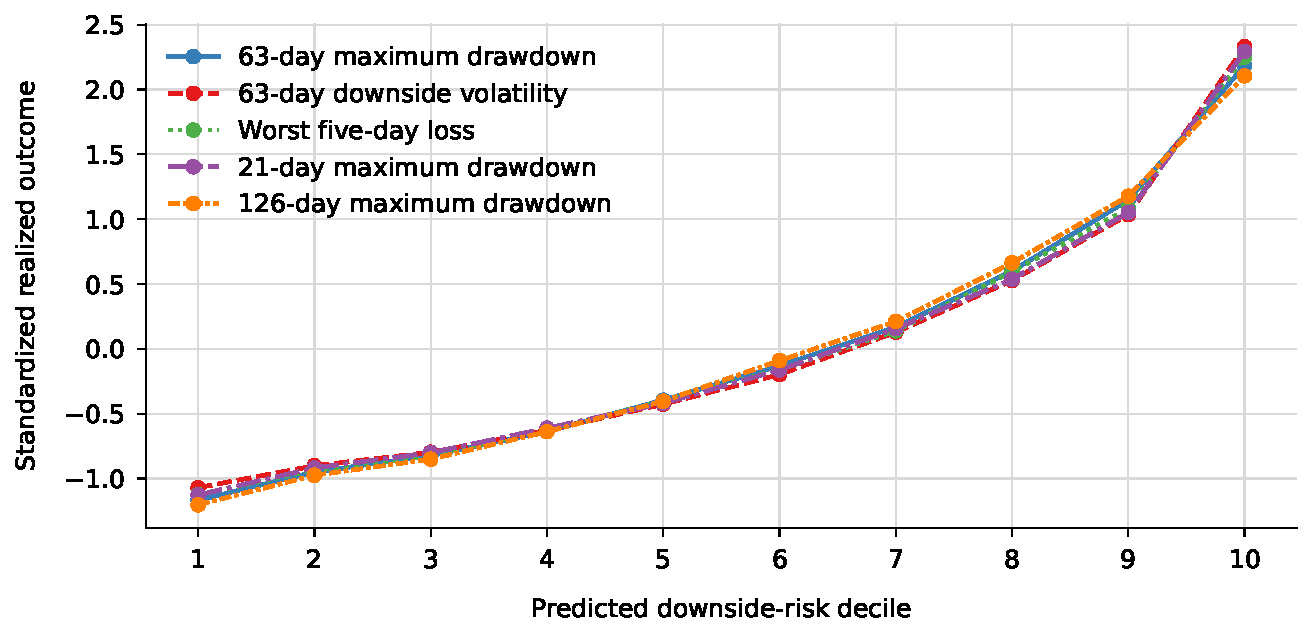
\includegraphics[width=0.88\textwidth]{04_10_xgboost_robustness_decile_profiles.pdf}
    \caption[Predicted-risk decile profiles across robustness targets]{Standardized realized outcomes across predicted-risk deciles for the primary and alternative targets.}
    \label{fig:app-predictive-robustness-deciles}
\end{figure}

\noindent
Figure~\ref{fig:app-predictive-robustness-quarterly-spearman} reports quarterly ranking performance for the primary and alternative targets. Figure~\ref{fig:app-predictive-robustness-quarterly-mae} reports each quarter's MAE relative to the corresponding target's overall test MAE.

\begin{figure}[!htbp]
    \centering
    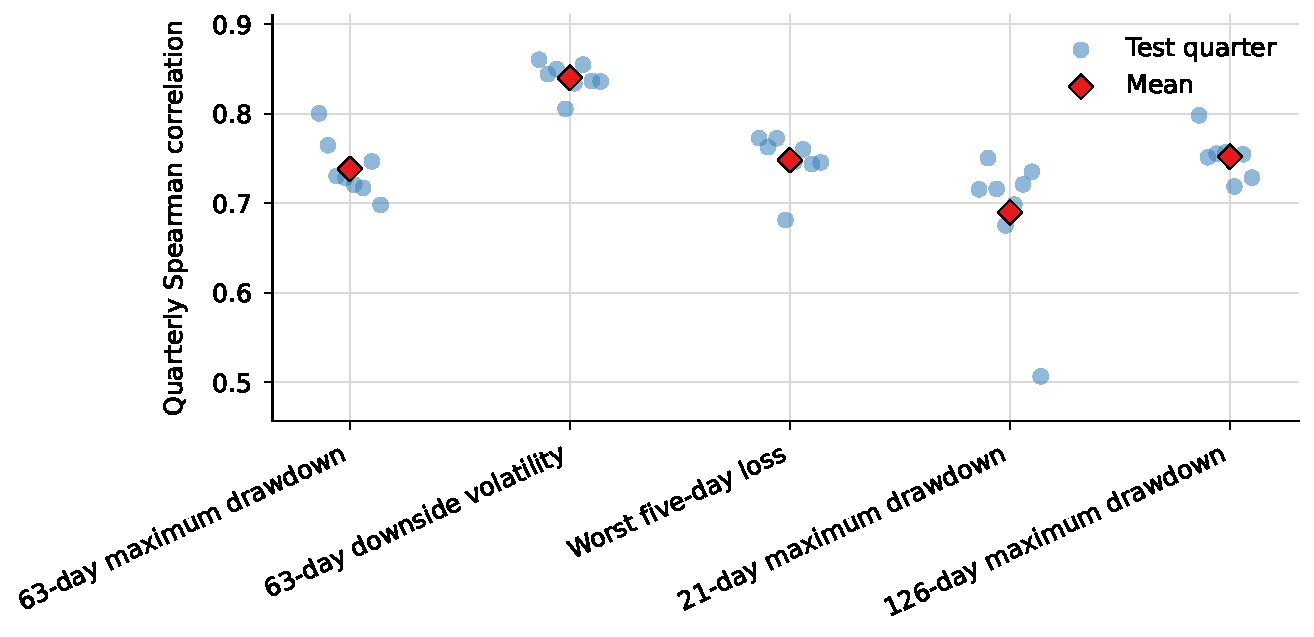
\includegraphics[width=0.82\textwidth]{04_10_xgboost_robustness_quarterly_spearman.pdf}
    \caption[Quarterly ranking performance across robustness targets]{Quarterly Spearman correlations between predicted and realized risk for the primary and alternative targets. Each point represents one test quarter, and diamonds mark the corresponding target means.}
    \label{fig:app-predictive-robustness-quarterly-spearman}
\end{figure}

\begin{figure}[!htbp]
    \centering
    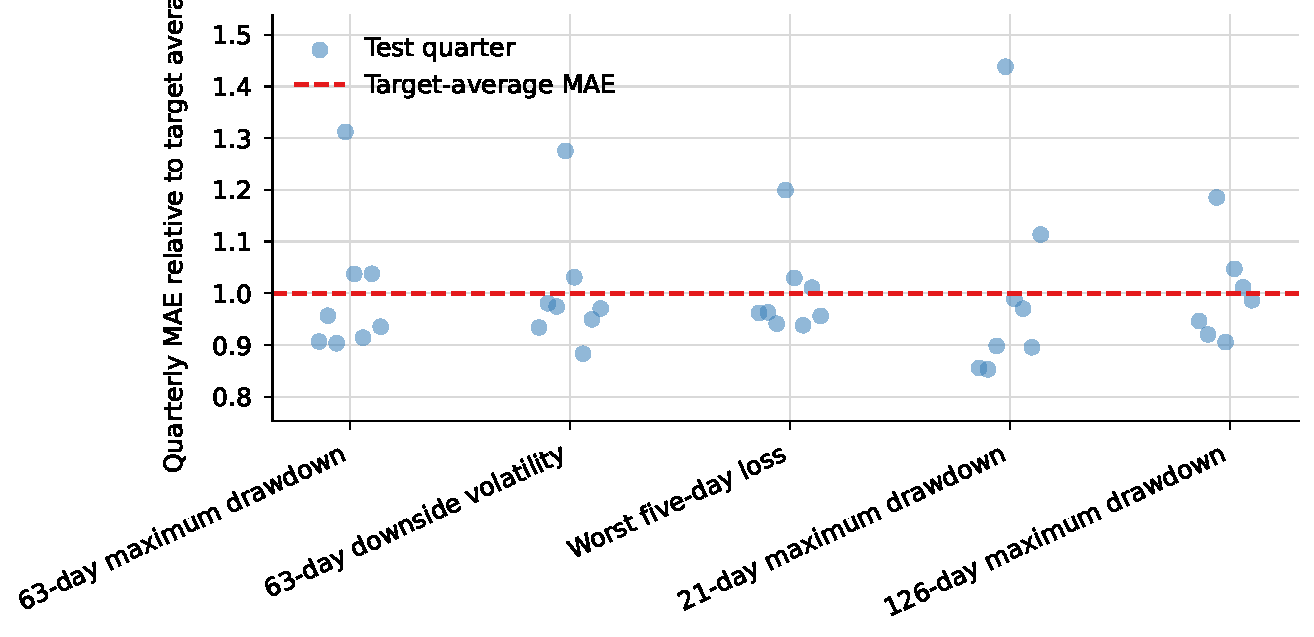
\includegraphics[width=0.82\textwidth]{04_10_xgboost_robustness_quarterly_relative_mae.pdf}
    \caption[Quarterly error stability across robustness targets]{Quarterly MAE relative to each target's overall test MAE. The dashed line at one denotes the target-specific average.}
    \label{fig:app-predictive-robustness-quarterly-mae}
\end{figure}

\section{Outcomes by Fragility Score Decile}
\label{app:fragility_score_supporting_outcomes}

Figure~\ref{fig:fragility-score-deciles} shows that predicted and realized maximum drawdown rise across Fragility Score deciles, with the strongest separation in the upper tail.

\begin{figure}[!htbp]
    \centering
    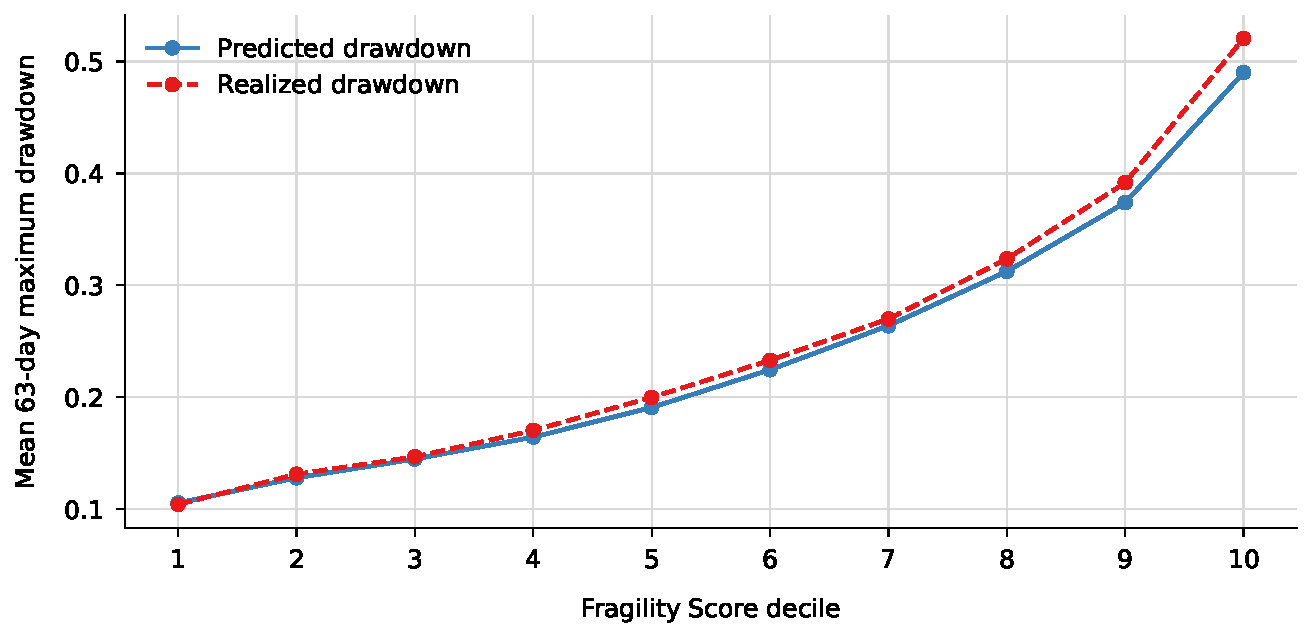
\includegraphics[width=0.78\textwidth]{04_11_fragility_score_deciles.pdf}
    \caption[Predicted and realized drawdown across Fragility Score deciles]{Mean predicted and realized 63-day maximum drawdown by within-quarter Fragility Score decile in the held-out sample.}
    \label{fig:fragility-score-deciles}
\end{figure}

\noindent
Figure~\ref{fig:app-fragility-score-supporting-outcomes} shows that higher Fragility Score deciles also exhibit greater realized downside volatility and worse five-day losses, while cumulative returns weaken toward the most fragile decile. The score therefore captures a broader downside-risk gradient rather than mechanically ranking only the primary maximum-drawdown target.

\begin{figure}[!htbp]
    \centering
    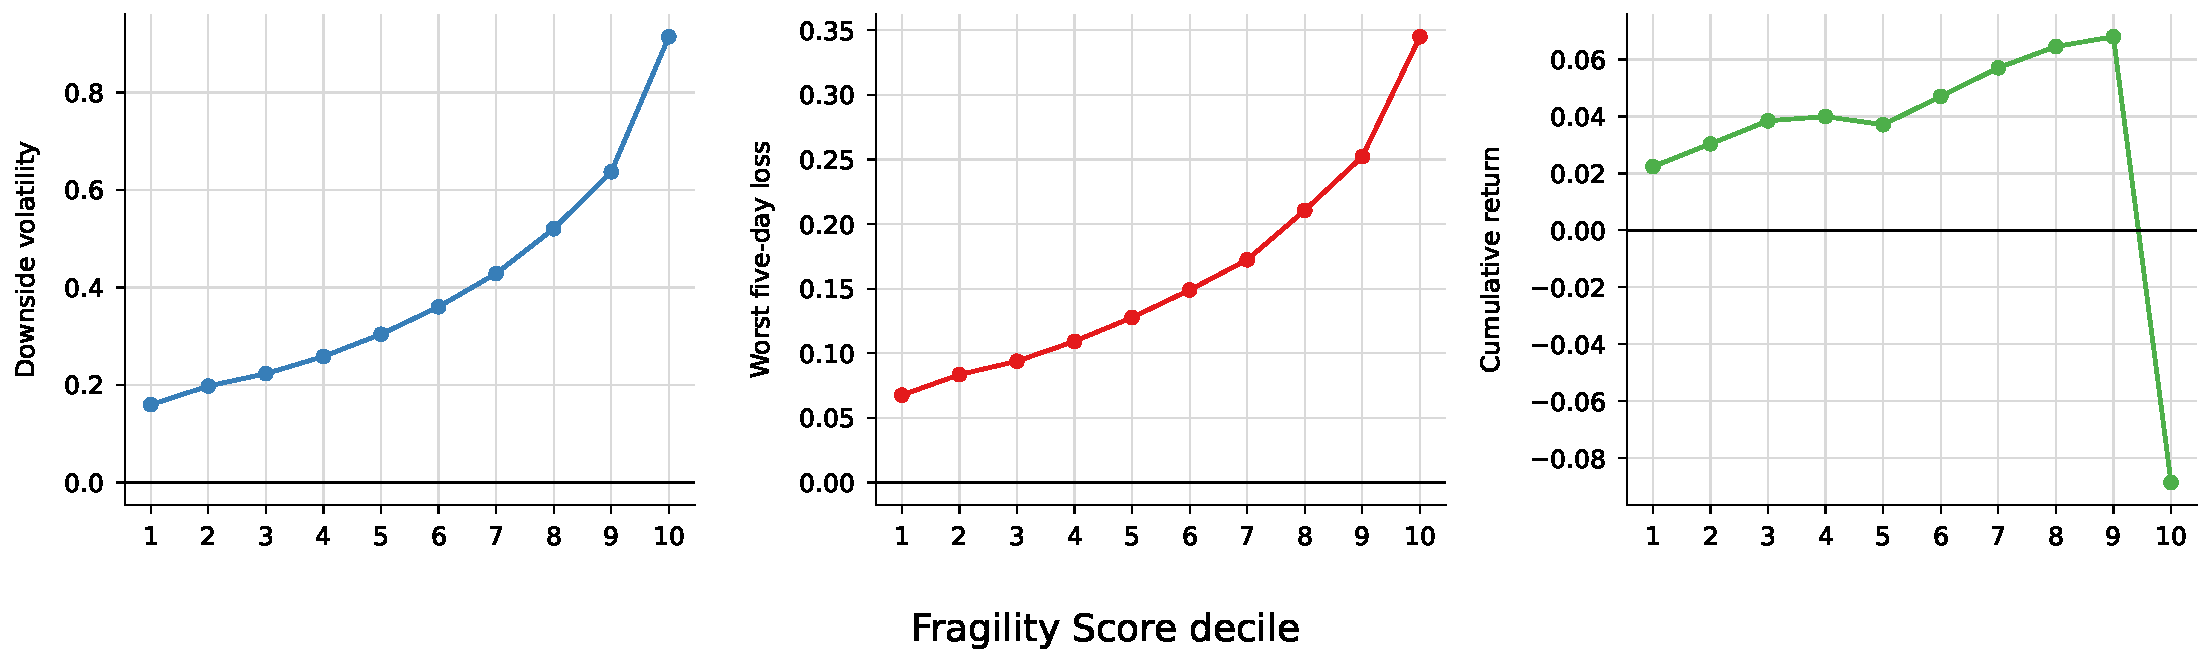
\includegraphics[width=\textwidth]{04_11_fragility_score_supporting_outcomes.pdf}
    \caption[Supporting outcomes across Fragility Score deciles]{Mean realized downside volatility, worst five-day loss, and cumulative return by within-quarter Fragility Score decile.}
    \label{fig:app-fragility-score-supporting-outcomes}
\end{figure}

\section{Primary Portfolio Factor Regressions}
\label{app:primary_portfolio_alpha}

Table~\ref{tab:portfolio-alpha} reports the complete FF5-plus-momentum regression statistics underlying Figure~\ref{fig:portfolio-strategy-alpha}.

\begin{table}[!htbp]
\centering
\footnotesize
\caption{FF5-plus-momentum alpha for the primary portfolio comparison.}
\label{tab:portfolio-alpha}
\begin{tabular}{lrrrr}
\toprule
Portfolio & Annualized alpha & $t$-statistic & $p$-value & Adjusted $R^2$ \\
\midrule
All eligible stocks & -5.2\% & -1.35 & 0.179 & 0.946 \\
Exclude Decile 10 & 0.0\% & 0.01 & 0.992 & 0.974 \\
Screened minus all stocks & 5.2\% & 2.77 & 0.006 & 0.174 \\
\bottomrule
\end{tabular}
\end{table}


\section{Quarterly Portfolio Risk Comparison}
\label{app:portfolio_window_risk}

Figure~\ref{fig:portfolio-event-window-risk} compares the average downside outcomes of the four primary portfolios across the quarterly holding windows. The screened portfolio improves modestly on the full equal-weighted universe, while the much larger separation between Decile~1 and Decile~10 confirms the score's economic ordering power.

\begin{figure}[!htbp]
    \centering
    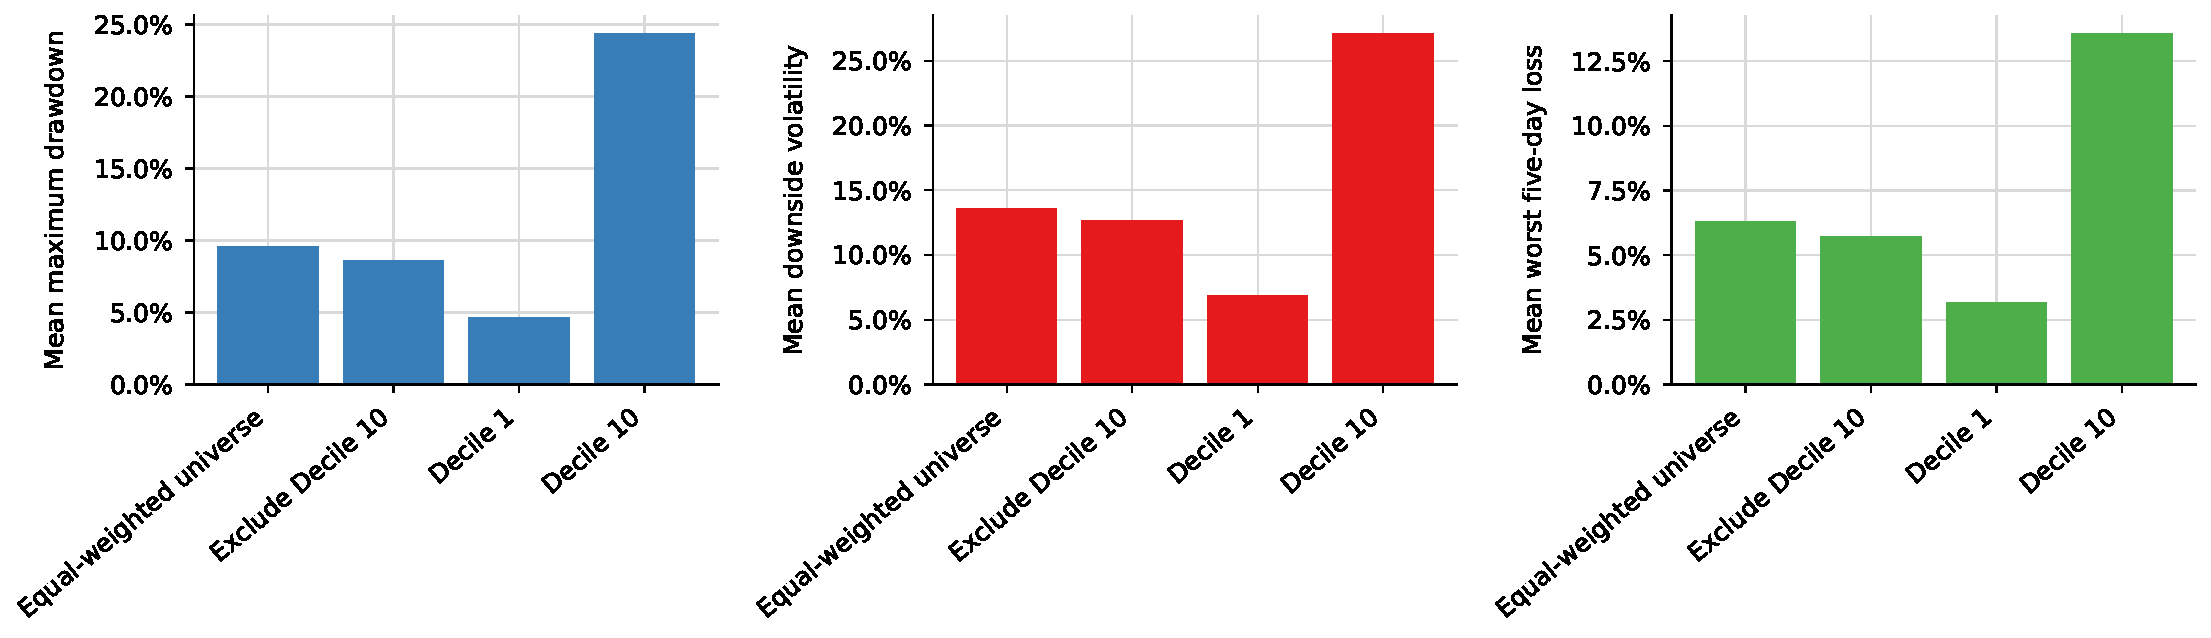
\includegraphics[width=\textwidth]{04_11_fragility_portfolio_risk.pdf}
    \caption[Risk across Fragility Score portfolios]{Average maximum drawdown, downside volatility, and worst five-day loss across the quarterly portfolio windows.}
    \label{fig:portfolio-event-window-risk}
\end{figure}

\section{Long-Only Portfolio Robustness}
\label{app:portfolio_robustness_figure}

Figure~\ref{fig:portfolio-robustness} compares the full and screened portfolios under alternative exclusion thresholds and weighting rules. The equal-weighted results remain similar when the exclusion threshold is widened, whereas the value-weighted portfolios are nearly unchanged by the screen.

\begin{figure}[!htbp]
    \centering
    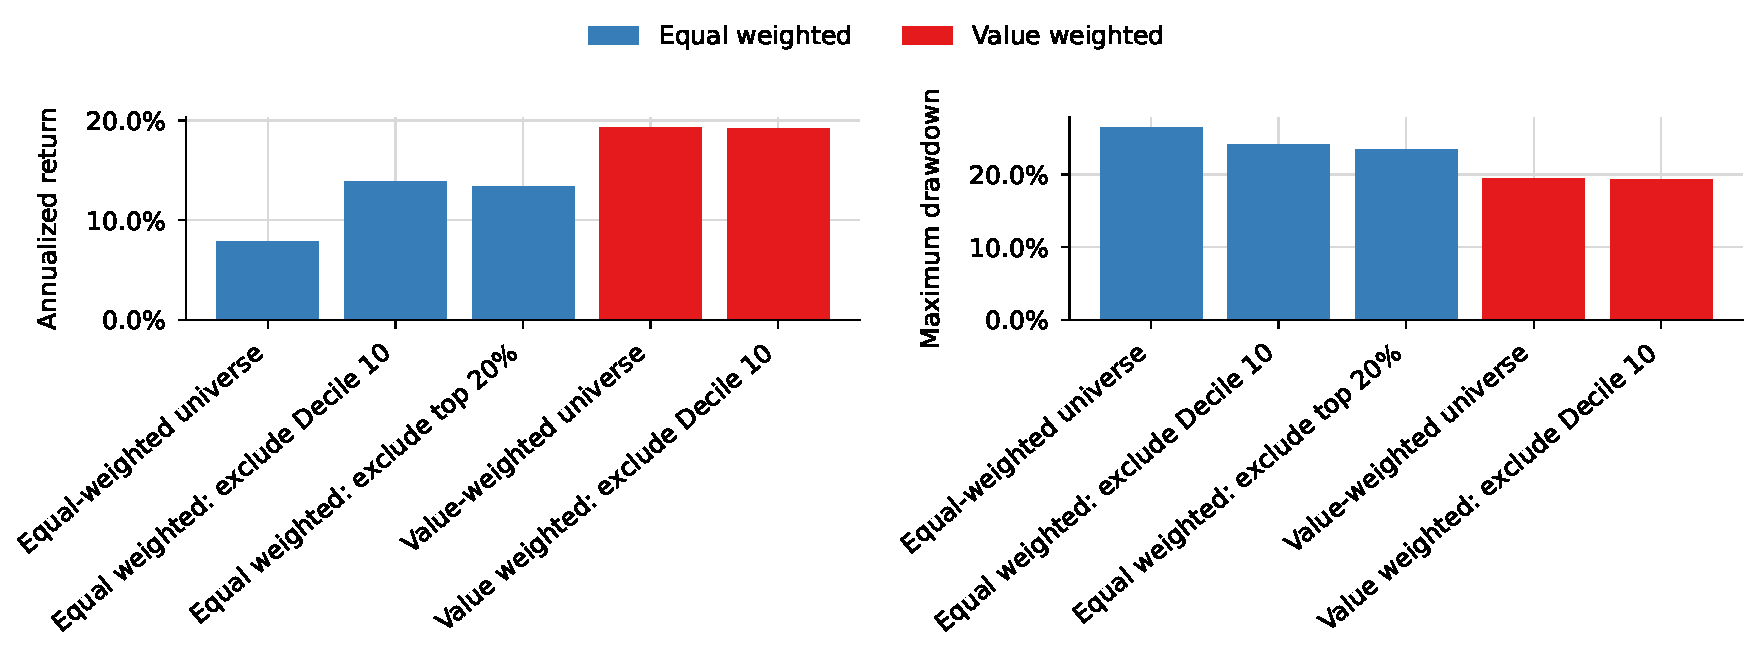
\includegraphics[width=\textwidth]{04_12_portfolio_robustness.pdf}
    \caption[Long-only portfolio robustness]{Performance of the full and screened portfolios under alternative exclusion thresholds and weighting rules.}
    \label{fig:portfolio-robustness}
\end{figure}

\section{Long--Short Transaction-Cost Sensitivity}
\label{app:long_short_cost_sensitivity}

Table~\ref{tab:long-short-cost-sensitivity} reports annualized returns under alternative one-way transaction-cost assumptions. The volatility-managed calculation includes turnover from both quarterly DFRAG-10 reconstitution and changes in volatility-targeted exposure. The range illustrates sensitivity to implementation costs rather than claiming that any single rate precisely represents realized trading costs.

\begin{table}[!htbp]
\centering
\footnotesize
\caption{Annualized returns of the long--short strategies under alternative one-way transaction-cost assumptions.}
\label{tab:long-short-cost-sensitivity}
\begin{tabular}{lrrrr}
\toprule
Strategy & Gross & 10 bps & 25 bps & 50 bps \\
\midrule
DFRAG-10 & 55.7\% & 55.1\% & 54.2\% & 52.7\% \\
DFRAG-20 & 16.0\% & 15.6\% & 15.0\% & 14.0\% \\
DFRAG-10: volatility managed & 28.2\% & 27.5\% & 26.5\% & 24.9\% \\
\bottomrule
\end{tabular}
\end{table}



% ==================================================
% ACKNOWLEDGEMENTS
% ==================================================

% Usually placed in the front matter, but this preserves
% your current backmatter directory choice.
%
% \chapter*{Acknowledgements}
% \addcontentsline{toc}{chapter}{Acknowledgements}
% \input{backmatter/acknowledgements}

\end{document}
